\documentclass[12pt, a4paper]{report}
\usepackage[english,vietnam]{babel}
%\usepackage[utf8]{inputenc}
\usepackage{booktabs}
\usepackage{array}
\usepackage{mathptmx}[ptm]
\usepackage{a4wide,amssymb,epsfig,latexsym,hhline,fancyhdr}
\usepackage[normalem]{ulem}
\usepackage{tabularx}
\usepackage[makeroom]{cancel}
\usepackage{amsmath}
\usepackage{amsthm}
\usepackage{multicol,longtable,amscd}
\usepackage{diagbox}%Make diagonal lines in tables
\usepackage{alltt}
\usepackage[framemethod=tikz]{mdframed}% For highlighting paragraph backgrounds
\usepackage{caption,subcaption}
\usepackage{float}

\usepackage{lastpage}
\usepackage[lined,boxed,commentsnumbered]{algorithm2e}
\usepackage{enumerate}
\usepackage{color}
\usepackage{graphicx}							% Standard graphics package
\usepackage{multirow}
\usepackage{rotating}
\usepackage{graphics}
\usepackage{geometry}
\usepackage{setspace}
\usepackage{tikz}

\usepackage{fontspec}
\usepackage[hyphens]{url}

\setmainfont{Times New Roman}

 
\usetikzlibrary{arrows,snakes,backgrounds,calc,positioning,shapes.geometric,shapes.misc}
\usepackage[unicode]{hyperref}
\hypersetup{
    colorlinks=true,
    linkcolor=blue,
    urlcolor=blue,
    citecolor=blue
}
\usepackage{listings}

%\usepackage{pstcol} 								% PSTricks with the standard color package


\usepackage{float}

\newtheorem{theorem}{{\bf Định lý}}
\newtheorem{property}{{\bf Tính chất}}
\newtheorem{proposition}{{\bf Mệnh đề}}
\newtheorem{corollary}[proposition]{{\bf Hệ quả}}
\newtheorem{lemma}[proposition]{{\bf Bổ đề}}
\theoremstyle{definition}
\newtheorem{exer}{Bài toán}
\addtocontents{toc}{\protect\thispagestyle{empty}}
% Remove page number in contents page. 
\addtocontents{lof}{\protect\thispagestyle{empty}}
% Remove page number in list of figure page. 
\addtocontents{lot}{\protect\thispagestyle{empty}}
% Remove page number in list of table page. 
\def\thesislayout{	% A4: 210 × 297
	\geometry{
		a4paper,
		total={160mm,240mm},  % fix over page
		left=30mm,
		top=22mm,
            right=20mm,
            bottom=20mm,
	}
}
\def\thesisheadlayout{	% A4: 210 × 297
	\geometry{
		a4paper,
		total={160mm,240mm},  % fix over page
		left=30mm,
		top=10mm,
	}
}
\thesislayout
\lstset{
language=R,
basicstyle=\footnotesize\sffamily,
commentstyle=\ttfamily\color{black},
numbers=left,
numberstyle=\ttfamily\color{black}\footnotesize,
stepnumber=1,
numbersep=5pt,
backgroundcolor=\color{white},
showspaces=false,
showstringspaces=false,
showtabs=false,
frame=single,
tabsize=2,
captionpos=b,
breaklines=true,
breakatwhitespace=false,
title=\lstname,
escapeinside={},
keywordstyle={},
morekeywords={}
}
%\usepackage{fancyhdr}
\setlength{\headheight}{40pt}
\pagestyle{fancy}
\fancyhead{} % clear all header fields
\renewcommand{\footruleskip}{1mm}

\fancyhead[L]{
 \begin{tabular}{rl}
    \begin{picture}(25,15)(0,0)
    \put(0,-8){
\includegraphics[width=10mm, height=10mm]{Images/hcmut.png}}
    %\put(0,-8){
\epsfig{width=10mm,figure=hcmut.eps}}
   \end{picture}&
	%
\includegraphics[width=8mm, height=8mm]{hcmut.png} & %
	\begin{tabular}{l}
		\textbf{  Ho Chi Minh University of Technology }\\
		\textbf{  Computer Science and Engineering Department}
	\end{tabular} 	
 \end{tabular}
}
\fancyhead[R]{
	\begin{tabular}{l}
		\tiny \bf \\
		\tiny \bf 
	\end{tabular}  }
\fancyfoot{} % clear all footer fields
\fancyfoot[L]{\scriptsize  Specialized Project Report (CO4029) - HK2 2025 - 2026}
\fancyfoot[R]{\scriptsize  Page {\thepage}/\pageref{LastPage}}

\renewcommand{\headrulewidth}{0.3pt}
\renewcommand{\footrulewidth}{0.3pt}

%%%
\setcounter{secnumdepth}{4}
\setcounter{tocdepth}{3}
\makeatletter
\newcounter {subsubsubsection}[subsubsection]
\renewcommand\thesubsubsubsection{\thesubsubsection .\@alph\c@subsubsubsection}
\newcommand\subsubsubsection{\@startsection{subsubsubsection}{4}{\z@}%
                                     {-3.25ex\@plus -1ex \@minus -.2ex}%
                                     {1.5ex \@plus .2ex}%
                                     {\normalfont\normalsize\bfseries}}
\newcommand*\l@subsubsubsection{\@dottedtocline{3}{10.0em}{4.1em}}
\newcommand*{\subsubsubsectionmark}[1]{}
\makeatother

\everymath{\color{black}}%make in-line maths symbols blue to read/check easily

\sloppy
\captionsetup[figure]{labelfont={small,bf},textfont={small,it},belowskip=-1pt,aboveskip=-9pt}
%space remove between caption, figure, and text
\captionsetup[table]{labelfont={small,bf},textfont={small,it},belowskip=-1pt,aboveskip=7pt}
\setlength{\floatsep}{5pt plus 2pt minus 2pt}
\setlength{\textfloatsep}{5pt plus 2pt minus 2pt}
\setlength{\intextsep}{10pt plus 2pt minus 2pt}

\thesislayout
\setlength{\parskip}{5pt plus 1pt minus 3pt}

\definecolor{S1blue}{RGB}{200,230,250}   % Station 1 blue
\definecolor{S1draw}{RGB}{30,120,180}    
\definecolor{workerOr}{RGB}{255,235,200} % Worker/Semaphore orange
\definecolor{workerDr}{RGB}{230,130,30}
\definecolor{queuePr}{RGB}{240,220,250} % Queue purple
\definecolor{queueDr}{RGB}{120,50,150}
\definecolor{builderGr}{RGB}{210,250,210} % Builder green
\definecolor{builderDr}{RGB}{40,150,40}
\definecolor{dbGrey}{RGB}{240,240,240}   % DB grey
\definecolor{dbDraw}{RGB}{100,100,100}


\begin{document}
\begin{titlepage}
\begin{tikzpicture}[remember picture, overlay]
  \draw[line width = 4pt] ($(current page.north west) + (0.4in,-0.5in)$) rectangle ($(current page.south east) + (-0.4in,0.5in)$);
  \draw[line width=1.5pt]
    ($ (current page.north west) + (0.45in,-0.55in) $)
    rectangle
    ($ (current page.south east) + (-0.45in,0.55in) $);
\end{tikzpicture}

\begin{center}
\LARGE \textbf{National University of Ho Chi Minh City} \\
\vspace{0.2cm}
\LARGE \textbf{HCM University of Technology} \\
\vspace{0.2cm}
\LARGE \textbf{Computer Science and Engineering Department}
\end{center}

\vspace{0.3cm}

\begin{figure}[h!]
\begin{center}

\includegraphics[width=4cm]{Images/hcmut.png}
\end{center}
\end{figure}

\begin{center}
    {\Huge \textbf{REPORT}} \\[0.5cm]
	{\LARGE \textbf{SPECIALIZED PROJECT}} \\
%    {\Huge \textbf{SmartEdu}} \\[1cm]
%    {\LARGE \textbf{A Graph-based Intelligent Teaching Assistant}} \\[0.5cm]
%    {\LARGE \textbf{for Mastery-oriented Learning Roadmap}} \\[0.5cm]
%    {\LARGE \textbf{Guidance and Supervision}} \\[1.5cm]
\noindent\rule{\linewidth}{0.5mm}
{\LARGE \textbf{RESEARCH AND DEVELOPMENT A SMART QUERY SOLUTION USING KNOWLEDGE GRAPH AND LANGUAGE MODELS}\\ }
\noindent\rule{\linewidth}{0.5mm}\\[0.5cm]
    {\Large Major: Computer Science}
\end{center}

\vspace{0.5cm}

\begin{tabular}{p{2.5cm} l l}
    & \textbf{\Large Thesis Committee:} & {\Large HĐ 3CC Đồ án chuyên ngành} \\[0.4cm]
    & \textbf{\Large Instructor:}       & {\Large Assoc. Prof. Thoại Nam} \\[0.4cm]
    & \textbf{\Large Secretary:}        & {\Large Mr. Lê Đình Thuận} \\[0.4cm]
    & \multicolumn{2}{c}{\textbf{\Large ---o0o---}} \\[0.4cm]
    & \textbf{\Large Student:}          & {\Large Vũ Hoàng Tùng (2252886)} \\
\end{tabular}
\vspace{0.5cm}
\begin{center}
{\Large HỒ CHÍ MINH City, June 2026 }
\end{center}
\end{titlepage}
%\thispagestyle{empty}
\newpage
%%%%%%%%%%%%%%%%%INTRO%%%%%%%%%%%%%%%%%%%
\section*{Acknowledgement}
\thispagestyle{empty}
This section is dedicated to express our sincere gratitude towards all those who have played a crucial role in the
completion of the Specialized Project, also the first phase of the thesis. Your supports have been a great help for
me to perform various steps from the fundamental researches and requirement specification to system design and implementation
development, laying foundations for the future Capstone Project
\\\\
I would like to show my foremost appreciation to my supervisor, Mr.Thoai Nam for his unwavering support, guidance and constructive feedback. His invaluable expertise and advice has really strengthened my vision and understanding, thus been instrumental in shaping the direction of my work.
\\\\
I am also greatly thankful to Computer Science Falcuty of Department for the learning environment, the facilities, the knowledge and the opportunity to orchestrate this work that I'm proud of. The contributions of my peers and colleagues in engaging discussions and shared insights have been enriching. 

To Bảo, a colleague and a friend of mine, whose knowledge and engaging discussion on system design has been a great help, I show my appreciation for his passionate and knowledgable share and consistent heart\-warming support.
\\\\
Finally, to all my family and friends who offered encouragement, shared their knowledge and gave inspiration 
%and especially those who shared years of teaching assistant experience
, I feel blessed that this Project and me have been supported by your love and care. 
\\\\
Last but not least, I acknowledge that this my work would not achieve the goal without the foundation laid by pioneering researchers and engineers, both in the field of 
artificial intelligence and education. The theories, methodologies, and technologies they have developed have been the bedrock upon which this project is built. 
The knowledge they have contributed is invaluable, and I am more than honored to stand on the shoulders of giants.
\\\\
This work stands firm thanks to the contribution of all those mentioned above. Your accumulated impact has been indispensible, and I cherish the roles each played in this academic endeavor. 
\clearpage
\pagenumbering{arabic}

\section*{DECLARATION OF AUTHENTICITY}
\thispagestyle{empty}

I guarantee that this specialized project entitled \textit{"SmartEdu: A Graph-based Intelligent Teaching Assistant for Mastery-oriented Learning Roadmap Guidance and Supervision"} was entirely composed and implemented by myself under the guidance and supervision of Assoc. Prof. Thoại Nam at the Faculty of Computer Science and Engineering, Vietnam National University - Ho Chi Minh City University of Technology.
\\\\Throughout the project, I ensure that all references and external sources utilized are appropriately cited and thoroughly documented. Although full code won't be included in report, important parts of the code will be summarizzed in pseudo form and referenced to source of inspiration (if yes).

\vspace{2cm}

\begin{flushright}
Ho Chi Minh City, May 2026 \\
\textbf{The author,} \\[0.5cm]
\textit{Vũ Hoàng Tùng}
\end{flushright}
\clearpage
\pagenumbering{arabic}

\section*{Abstract}
\thispagestyle{empty}
Current world is changing at an incredible pace with constant information and knowledge update, while many educational systems remain stagnant. The rapid evolution of 
Artificial Intelligence has open doors for adaptive, self-directed learning online systems, replacing Learning Management Systems that offer static contents. 
However, common AI techniques such as Retrieval-Augmented Generation (RAG) struggle with static content, semantic fragmentation, and a lack of profound reasoning, while LLMs have limited 
context window and hallucination, inconsistent output.

To address these limitations, this project introduces \textbf{SmartEdu}, a proactive, mastery-oriented educational ecosystem powered by a graph-grounded multi-agent 
architecture.
By operating LLM on deterministic ingesting pipeline for academic materials, the system constructs an Automated Educational Knowledge Graph (EKG) that accurately 
maps conceptual hierarchies and prerequisite dependencies.  
Unstructured multimodal materials are automatically ingested via an asynchronous Producer-Consumer pipeline and processed through a novel Dual-Phase LLM extraction 
technique. This is reinforced by deterministic NLP filtering—including DBpedia validation and implicit clustering—to ensure strict ontological hierarchy and 
prerequisite acyclic constraints.

For real-time tutoring, a LangGraph-driven Teaching Assistant operates within an Adaptive Middleware harness, strictly separating reasoning contexts and action schemas. 
It utilizes Knowedge Graph as a well\-structured ground truth and solid reasoning frame, cooperates open-weights Small Language Models (SLMs) into workflow 
for localized and privacy-preserving execution, and
orchestrates specialized multi-agent workflows—Retrieve, Roadmap, and Teach—to perform dynamic student mastery tracking, automated gap detection
using topological algorithms, and personalized learning pathfinding, all while safeguarding student privacy and important resources through a robust 
Indentity-Session dynamic allocation and management.

Initial evaluations of the system demonstrate successful and consistent AI operations, effectively reduce hallucinations, produce consistent results and reasoning, and 
maintaining structural integrity across complex academic domains. Despite current latency bottlenecks and challenges in macro-level course pathing, 
SmartEdu establishes a robust, highly scalable foundation for shifting the educational paradigm from linear content delivery to interactive, 
human-like mentorship.

The project is being actively maintained on Github: \url{https://github.com/ttb-hcmut/SmartEdu}

\clearpage
\pagenumbering{arabic}

\newpage
\tableofcontents
\newpage
\listoffigures
\newpage
\listoftables
\newpage
\setcounter{page}{1}

%%%%%%%%%%%%%%%%%CONTENTS%%%%%%%%%%%%%%%%%%%
\chapter{Introduction}

\section{Motivation}

The rapid evolution of Artificial Intelligence (AI) has fundamentally change the global socio-economic landscape. To adapt to the new era, self\-studying and learning method are becoming more and more important. Traditional education philosophy, such as "practice makes perfect," has no longer been the absolute true; when AI can automate execution, the value of learning moves from procedural fluency and labour expertise to conceptual mastery and strategic analysis. However, current education system fail to keep pace with this evolution:

\begin{itemize}
    \item \textbf{Stagnancy of Content:} Legacy Learning Management Systems (LMS) treat knowledge as static artifacts (textbooks, slides). These materials fail to adapt to the varying cognitive baselines of individual students.
    \item \textbf{The Guidance Deficit:} Without a dynamic roadmap, students navigate a "sea of information" where external resources are either too granular (leading to information overload) or too condensed (creating knowledge gaps), with little profound ground truth.
    \item \textbf{The Lack of Interaction:} Current systems lack a feedback loop. Textbooks exceed the average human attention span, while slides provide too condensed context insufficient for novices, leaving no room for real-time, human-like inquiry or mentorship.
    \item \textbf{Outdated Knowledge:} Educational materials and methods cannot catch up with the change of technology. Internet are an invaluable resource, however information is chaotic, unstructured and content are confusing to many new learners.
\end{itemize}

While Large Language Models (LLMs) offer a glimpse into automated resource synthesis and knowledge base construction, significant technical bottleneck prevent their reliable application in complex domains:

\begin{itemize}
    \item \textbf{Semantic Fragmentation in RAG:} Traditional Retrieval-Augmented Generation (RAG) frameworks rely on discrete data chunking. This fragmentation disrupts the global structural integrity of a subject, leading to "contextual myopia" where the model captures isolated facts but fails to comprehend the overarching hierarchy of the domain.
    \item \textbf{Contextual Saturation vs. Precision:} Expanding the context window of LLMs often introduces diminishing returns. The injection of unrefined data frequently leads to "contextual overhead" and "noise," where the model struggles to distinguish fundamental principles from peripheral details.
    \item \textbf{Relational Limitations of Vector Space:} Relying exclusively on vector embeddings (typically $\approx 1024$ dimensions) is insufficient for mapping the non-linear, multi-faceted dependencies inherent in academic taxonomies. Similarity-based retrieval cannot substitute for the deterministic logic required to understand prerequisite relationships.
    \item \textbf{The Reasoning Gap in Pedagogy:} Instruction is a sophisticated, non-linear reasoning task. Current AI systems are largely reactive—proficient in text generation but deficient in long-term goal tracking and proactive guidance. This results in a susceptibility to hallucinations and an inability to execute the "evaluate-and-guide" workflow essential for effective pedagogy.
\end{itemize}

\section{Goals}

This project aims to bridge the gap between passive content and active learning by developing a personalized AI-driven educational ecosystem. The specific objectives include:

\begin{itemize}
    \item \textbf{Philosophy of Co-living with AI:} Transforming AI from a simple tool into a pervasive personal assistant that evolves alongside the learner.
    \item \textbf{Cognitive State Tracking:} Establishing a system to record student progress, identify long-term goals, and objectively evaluate theoretical comprehension through interaction.
    \item \textbf{Adaptive Learning Trajectories:} Customizing the learning pace and curriculum dynamically, ensuring that the difficulty level remains within the student's "Zone of Proximal Development."
\end{itemize}

\section{Scope}

To fulfill these goals, the research focuses on the following technical cores:

\begin{itemize}
    \item \textbf{Knowledge Modeling:} Developing a deterministic "Backbone Graph" that maps semantic connections and context grouping, serving as a structural pattern for LLM reasoning. 
    \item \textbf{Context Engineering:} Engineering methods to facilitate reasoning across vast, high-density knowledge bases without losing global coherence.
    \item \textbf{Agent Workflow Orchestration:} Designing multi-agent systems to handle complex, multi-step pedagogical reasoning tasks.
    \item \textbf{Systemic Architecture:} Implementing clean design patterns optimized for scalable, AI-native educational services.
    \item \textbf{User Experience (UX):} Creating a dual-interface system featuring real-time agent streaming for interaction and a comprehensive GUI for administrative and roadmap visualization.
\end{itemize}


\section{Thesis structure}
There are 7 chapters in this project's report:

\begin{itemize}
    \item \textbf{Chapter 1} introduces the problems, proposes the system's goals, scopes and thesis structure
    \item \textbf{Chapter 2} provides fundamental knowledge for project understand and deep literature review of relevant prior researches covering topic, as well as preview of open-source application.
    \item \textbf{Chapter 3} Requirement Specifications
    \item \textbf{Chapter 4} propose methodologies: we discuss what inferred from previous work and what ways to solve the specific usecase of ours
    \item \textbf{Chapter 5} details the system including: System architecture and its components, settings in each components, and finally, their implementation explanation that fully illustrate how do the system put proposed methodology to practice 
    \item \textbf{Chapter 6} analyzes the system outcomes from components to final output as a whole
    \item \textbf{Chapter 7} is the conclusion to the result: what the system achieved, its limitation and future improvements for the final Capstone Project
\end{itemize}
\newpage
\chapter{Fundamental Knowledge \& Related Work}
\section{Fundamental Knowledge}
This section discusses the fundamental techniques and applications foundational to the construction of the proposed system, categorized into 3 pillars: 
\begin{itemize}
    \item {Natural Language Processing (NLP):} The foundational process of transforming vast volumes of raw, unstructured textual input into logical, structured 
    data formats that machine can understand. This is fundamental for document processing, reshaping all subsequent cognitive actions.
    \item {Large Language Models (LLMs)}: The core reasoning and action components of the system, responsible for interpreting user queries, orchestrating tools, and generating responses. This pillar represents the "intelligence" of the system, enabling it to perform complex tasks and adapt to user needs.
    \item {Agentic Orchestration:} The management layer responsible for coordinating specialized AI agents to execute complex, non-linear  workflows.
    \item {System Design:} The architectural blueprint that ensures scalability and robustness, utilizing clean design patterns tailored for high-stakes educational environments.
\end{itemize}
\subsection{Natural Language Processing}

Natural Language Processing (NLP) is a crucial field of study aiming to process unstructured data from documents to a structured, semantically rich representation. This process is designed to harness the full potential of complex entity-relationship paradigms, moving from raw text to machine-inferable logic. As outlined in the core objectives of language understanding, the goal is to put information into a semantically precise form that allows for further inferences.

The standard pipeline for Natural Language Processing follows the sequence:
\begin{center}
    {Information Extraction (IE) $\longrightarrow$ Knowledge Modeling $\longrightarrow$ Information Retrieval}
\end{center}

\subsubsection*{Information Extraction (IE)}
Information Extraction is the task of identifying and understanding limited, relevant portions of a text to produce a structured representation~\cite{StanfordNLP}. Its goal is to filter out linguistic noise and isolate the atomic units of knowledge. Traditional algorithms aim to extract keywords, following thế 2 methods:

\begin{itemize}
    \item {Keyword and Feature Extraction:} Utilizing dependency parsing and statistical methods (e.g., TF-IDF) to identify high-signal terms based on syntactic importance.
    \item {Named Entity Recognition (NER):} A critical sub-task used to find and classify concepts or entities (e.g., specific academic theories, formulas, or historical figures) within a text database~\cite{StanfordNLP}. This identifies the "nodes" of our future backbone.
\end{itemize}

To capture complex entities and relationships that rigid rule-based systems miss, the process relies on probabilistic modeling. The foundation of this approach is 
Tokenization, which breaks down raw text into atomic units (tokens). Statistical algorithms, such as Conditional Random Fields (CRF) or Hidden Markov Models (HMM), 
are then applied to these tokens to calculate the probability distribution of various interpretations. This allows the system to resolve linguistic ambiguities and 
predict the most likely semantic structures or labels for sequences of text.

While traditional probabilistic models logically and practically work in many usecases, they often struggle with sparse data and lack deep semantic understanding. 
Deep Learning represents a significant advancement by shifting the target towards generating Embeddings. Instead of merely calculating discrete probabilities, Deep Learning 
architectures map tokens into a continuous, high-dimensional vector space. In this embedding space, geometrically close vectors represent semantically related concepts, 
allowing the system to grasp the underlying meaning, context, and nuance of the information rather than relying solely on surface-level statistics.
\begin{figure}[H]
    \centering
    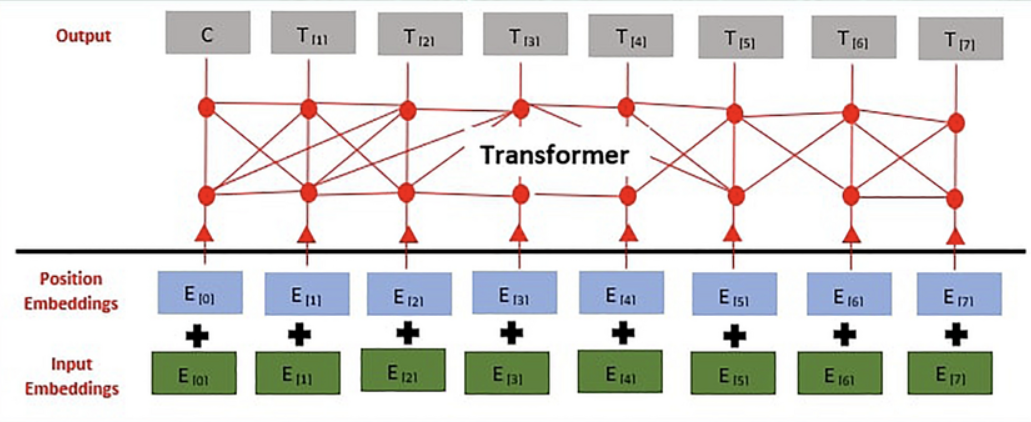
\includegraphics[width=0.7\textwidth]{Images/fundamental/embedding.png}
    \vspace{12pt}\caption{Transformer turn unstructured raw text into embeddings---numeric representation that hypothetically capture the core semantic}\label{fig:trans_embedding}
\end{figure}
The Transformer architecture was introduced, being SOTAs as well as standard method nowadays. It fundamentally change the landscape 
of NLP and enable modern Large Language Models (LLMs). The core innovation of the Transformer is the Attention Mechanism (specifically, Self-Attention). Instead of 
processing tokens sequentially, Transformers process the entire sequence simultaneously. The Attention Mechanism calculates a weighted importance score for every 
token relative to every other token in the sequence, regardless of their distance. This allows the model to instantly capture global context and long-range 
dependencies, making it the most powerful method for extracting deep, complex information from unstructured texts.

\subsubsection*{Knowledge Modeling}
Often overlooked in standard RAG systems, Knowledge Modeling is the construction stage where extracted entities are organized into a coherent structure that shapes how the system perceives and reasons.

\begin{itemize}
    \item {Semantic Parsing and Logical Form:} Mapping extracted relations into a semantically precise form, such as First-Order Predicate Calculus (FOPC) or 
    Knowledge Graphs (KG). This creates a deterministic "Backbone Graph" of the curriculum.
    \item {Embedding Space Topology:} Modeling knowledge within a continuous vector space where semantic similarity is represented by geometric proximity. 
    This allows the system to handle concepts that are conceptually related but lexically distinct.
\end{itemize}

\subsubsection*{Information Retrieval (IR)}
Information Retrieval is the active execution stage based on the result of construction phases IE and Knowledge Modeling, where the goal is to identify documents or data points relevant to a specific information need from a large document set~\cite{StanfordNLP}.

\begin{itemize}
    \item {Lexical and Keyword Matching:} Corresponding to traditional IE, this method uses exact term overlaps to find specific references or symbolic links 
    within the knowledge base.
    \item {Vector Retrieval:} the most common modern approach, utilizing the embedding space to retrieve context based on semantic similarity, typically 
    calculated via Cosine Similarity:
    \begin{equation}
        \text{similarity}(\mathbf{A}, \mathbf{B}) = \frac{\mathbf{A} \cdot \mathbf{B}}{\|\mathbf{A}\| \|\mathbf{B}\|}
    \end{equation}
    \item {The GraphRAG Paradigm:} A new powerful emerging method, where retrieval navigates the entity-relationship graph established during the modeling phase. Unlike discrete chunk retrieval, GraphRAG performs "multi-hop" reasoning to connect disparate concepts, enabling the system to resolve complex queries that require a global understanding of the educational roadmap.
\end{itemize}


\subsection{Large Language Models (LLMs)}

Large Language Models (LLMs) are deep learning-based probabilistic models trained on massive datasets to understand and generate human-like text. Mathematically, an LLM performs the task of next-token prediction by modeling the conditional probability distribution of a token $w_{t}$ given a sequence of preceding tokens $(w_{1}, w_{2}, \dots, w_{t-1})$:

\begin{equation}
P(w_{t} | w_{1}, w_{2}, \dots, w_{t-1})
\end{equation}

The structural foundation of modern LLMs is the {Transformer} architecture, which relies on the {Self-Attention} mechanism. This mechanism allows the model to compute the relative importance of different tokens in a sequence regardless of their distance. The attention score is calculated using Query ($Q$), Key ($K$), and Value ($V$) matrices derived from input embeddings:

\begin{equation}
Attention(Q, K, V) = \text{softmax}\left(\frac{QK^T}{\sqrt{d_k}}\right)V
\end{equation}

By utilizing multi-head attention and positional encoding, Transformers can capture complex linguistic patterns and long-range dependencies more effectively than previous sequential architectures like Recurrent Neural Networks (RNNs).



[Image of Transformer architecture diagram]


\subsubsection*{LLM Ecosystem: Proprietary vs Open-Weights}

The landscape of Large Language Models in the industrial layer (not research layer) is categorized by deployment strategies and the degree of architectural transparency. Closed-source and 
cloud-based models, such as GPT-4 and Claude, represent the proprietary tier of this ecosystem. These models are typically provided as a Service (SaaS), where interactions 
occur via Application Programming Interfaces (APIs) hosted on centralized, high-performance infrastructures. While these proprietary solutions consistently deliver 
state-of-the-art performance across a wide range of benchmarks, their internal mechanisms—including model weights, training datasets, and specific configurations—remain 
opaque. Furthermore, their operational use often involves per-token costs, which can become a significant factor in large-scale or iterative research applications.
\begin{figure}[H]
    \centering
    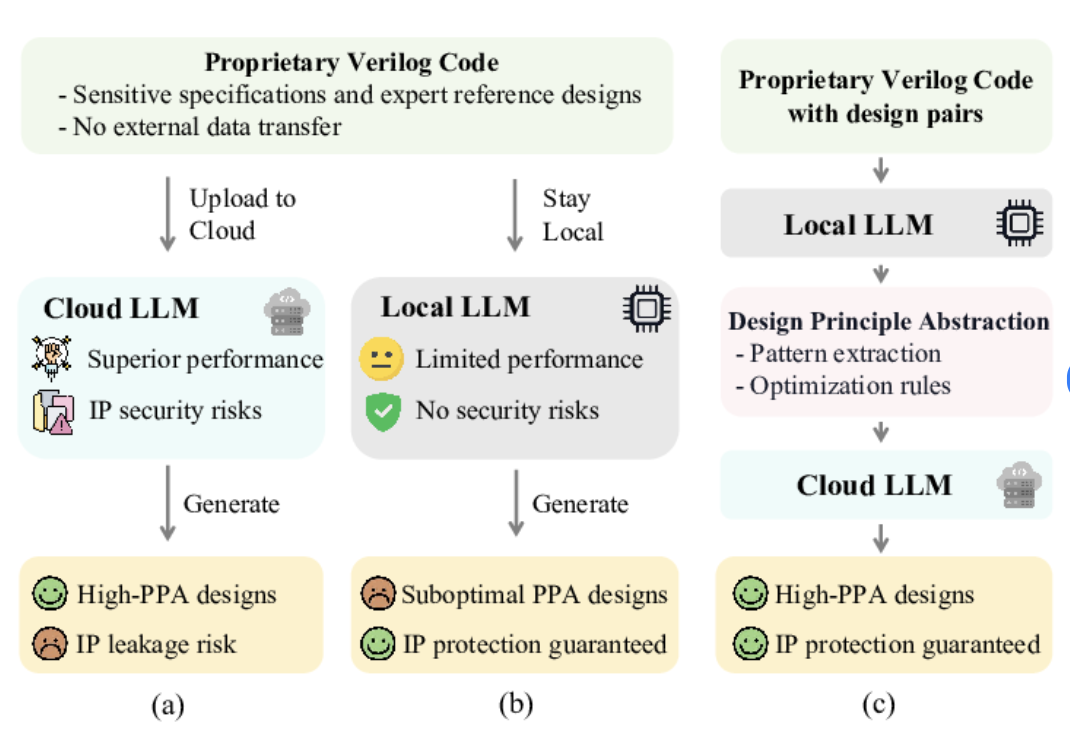
\includegraphics[width=0.7\textwidth]{Images/fundamental/cloud_local_llm.png}
    \vspace{12pt}\caption{Comparison of LLM Deployment Strategies: Traditional approaches (a) Direct cloud processing, (b) Local-only processing, and (c) Local-Cloud framework balance performance\-security without leaking IP (proposed by~\cite{IP_Safe_llm})}\label{fig:cloud_local_llm}
\end{figure}
\\
In contrast to the proprietary paradigm, the emergence of open-weights and local models has introduced a significant shift toward decentralized execution and 
architectural transparency. Initiatives such as Meta’s Llama series and Mistral release their pre-trained model parameters to the public, allowing for deployment 
on private, local infrastructures. This transparency facilitates full control over data sovereignty and privacy, as information does not need to leave the local 
environment to be processed. Consequently, these models serve as foundational baselines, providing a stable platform for both academic research and industrial 
innovation without the necessity of external API dependencies or recurring subscription fees.

Building upon these general-purpose baselines, recent advancements in the field have catalyzed a trend toward specialization, 
where models are fine-tuned or structurally modified for high-performance niche tasks. One prominent example is the development 
of coding specialists, such as Qwen-coder or CodeLlama, which are optimized specifically for source code synthesis and complex 
logical reasoning. These specialized variants often rival or even outperform significantly larger general-purpose models in 
programming-centric contexts. Beyond text processing, research has also extended these baseline architectures into the multimodal 
and generative domains. By integrating vision encoders for visual comprehension or combining LLM backbones with diffusion-based architectures, researchers have developed sophisticated models capable of high-fidelity image generation and cross-modal reasoning.

\subsubsection*{LLM Inference}

This subsection explains the utility of LLM inference parameters in controlling the generation process. During inference, the next-token probability distribution predicted by the model can be dynamically altered to balance determinism and creativity.

\paragraph*{Temperature}
Temperature ($\tau$) controls the sharpness or randomness of the predicted probability distribution. Given the logits $z_i$ output by the final layer, the adjusted probability $P(w_i)$ for each candidate token is computed using the modified softmax function:
\begin{equation}
P(w_i) = \frac{\exp(z_i / \tau)}{\sum_{j} \exp(z_j / \tau)}
\end{equation}
A lower temperature ($\tau < 1$) sharpens the distribution, making the model more confident in its top choices and producing highly deterministic text, which is ideal for rigid tasks like JSON extraction. A higher temperature ($\tau > 1$) flattens the distribution, encouraging diversity and creativity.

\paragraph*{Top-k Sampling}
Top-$k$ sampling restricts the model from considering the entire vocabulary, instead keeping only the $k$ highest-probability candidates. This approach is conceptually similar to beam search, where only the most promising paths are kept active:
\begin{equation}
V_k = \mathop{\mathrm{arg\,max}}\limits_{V' \subset V, |V'|=k} \sum_{w \in V'} P(w)
\end{equation}
The probability mass is then redistributed among these $k$ tokens. This truncation prevents the model from generating highly improbable and potentially nonsensical words (the "long tail" of the distribution).

\paragraph*{Top-p (Nucleus) Sampling}
Top-$p$ (nucleus) sampling provides a dynamic alternative to Top-$k$. Instead of keeping a fixed number of tokens, it keeps the smallest prefix subset of the vocabulary whose cumulative probability mass meets or exceeds a threshold $p$:
\begin{equation}
\min \left\{ |V'| : V' \subset V, \sum_{w \in V'} P(w) \geq p \right\}
\end{equation}
This allows the candidate pool to expand or contract organically based on the model's confidence. When the model is very confident, the nucleus contains only a few tokens; when uncertain, the nucleus expands to include more options.

\paragraph*{Repetition Penalty}
Repetition penalty modifies the logits of tokens that have already appeared in the generated sequence, mathematically reducing their likelihood of being selected again. This is crucial for preventing the model from entering infinite generation loops or excessively repeating specific phrases, ensuring a more natural and progressive text flow.


\subsection{Agentic Systems}

\subsubsection*{AI Agents: Definition and Capabilities}
An Artificial Intelligence (AI) Agent is a computational system capable of autonomous task execution through the dynamic design of workflows using available tools. 
AI agents can encompass a wide range of functions beyond natural language processing including decision-making, problem-solving, interacting with external environments, and performing actions.


\begin{figure}[H]
    \centering
    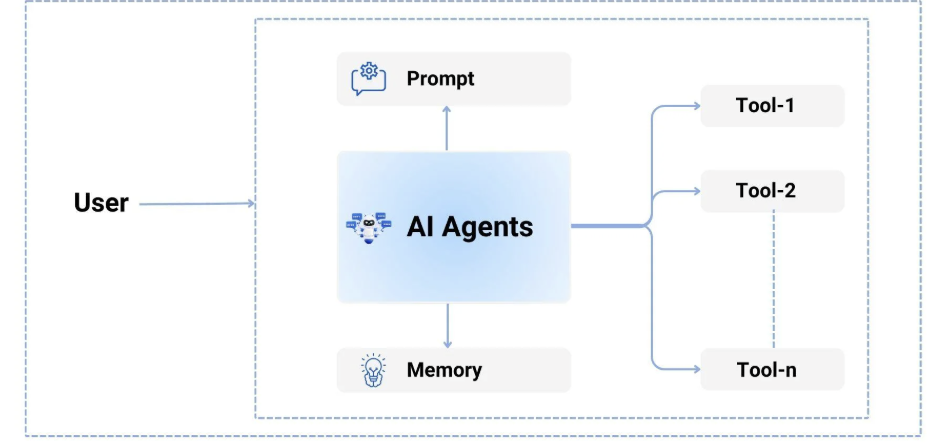
\includegraphics[width=0.6\textwidth]{Images/fundamental/agent.png}
    \vspace{12pt}\caption{Basic Single Agent diagram}\label{fig:react}
\end{figure}

Unlike Large Language Models (LLMs), which produce responses solely based on the static data used to train them and are bounded by fixed knowledge limits, agentic 
technology uses tool calling on the backend to obtain up-to-date information. They optimize workflows and create subtasks autonomously to achieve complex goals. It is 
responsible for translating high-level natural language queries into executable workflows. Instead of relying on rigid, pre-programmed paths, the agent dynamically 
analyzes the request, identifies the necessary tools, and orchestrates them in a sequence that best addresses the user's needs. This allows for a more flexible and 
adaptive system that can handle a wide variety of queries and tasks without requiring explicit programming for each scenario. 

What truly pushing agentic systems to achive what LLM can't lies in the harnessing of agentic technology. Harness is the process of constructing and integrating 
systems or infrastructure that boosts capabilities into the system. The harnessing of agentic system is critical for the agentic performance, as it enables the system 
to navigate the complex, multi-step processes required to analyze and retrieve relevant educational content based on user queries.
\paragraph*{LLM: The Logical Core}
Large Language Models (LLMs) serve as the brain of the agent, represent the thinking capability. They provide the reasoning capabilities necessary to interpret vague user queries and orchestrate the appropriate tools to find answers. The LLM is responsible for parsing the user's intent, identifying missing information, and deciding on the next actions. The reasoning and decision-making depend heavily on the type of LLM used. Upon studying the current industry, mainstream types of models include:
\begin{itemize}
    \item {Reasoning Models: }
Models such as OpenAI o1 or DeepSeek R1 are optimized for Chain of Thought processing. They excel at complex logical deduction and planning multi-step workflows before taking action. This makes them ideal for the planning phase, where they must decompose difficult user queries into a clear, executable plan before invoking any tools.
    \item {Function Calling Models}
Models such as GPT-4o or Claude 3.5 Sonnet are fine-tuned specifically to output structured data, such as JSON, rather than just conversational text. This capability is efficient for tool configuration and defining output formats. They are critical for the execution phase, as they can reliably select the correct tools and format the arguments precisely to query the database without syntax errors.
    \item {Multimodal Models}
    Models such as Gemini 1.5 Pro are trained with multimodal input. These models are essential in an educational content analysis context because they can natively understand both text and visual inputs. This allows the agent to process image frames directly alongside the user's text query without needing a separate description tool to translate visuals into text first.
    
    \item{Lightweight Efficiency Models}
    Smaller models like Llama 3 8B or GPT-4o-mini are faster and cheaper to run. They are perfect for narrow, repetitive tasks such as summarizing retrieved results or classifying user intent, where the deep reasoning capabilities of a larger model are unnecessary. Moreover, the ability to easily train and fine-tune these models facilitates customization in the design of Agentic systems.
\end{itemize}



\paragraph*{Context Engineering}
Context engineering, represent the memorization capacity, involves crafting the environment in which the LLM operates to ensure accurate and consistent outputs. This field includes several topics that govern how the model interacts with data and users.
\begin{itemize} 

\item {Prompting Strategies}
Prompting is the primary method to instruct the agent, helping it understand the goals and constraints it is dealing with. Techniques such as Query Expansion allow the agent to broaden search terms for better recall. Advanced methods like Chain of Thought (CoT) and Language of Thought (LoT) prompt the agent to articulate its reasoning process step-by-step, ensuring that complex logic is handled systematically before a final answer is generated.

\item {State Management}
To maintain a coherent interaction, systems must store chat history and the current state. This allows the agent to understand follow-up questions, such as "What happened after that?", by recalling the context of previous turns. State management ensures the agent knows exactly where it is in a multi-step retrieval process, preventing redundant actions.

\item {Retrieval-Augmented Generation (RAG)}
Agents cannot remember all the information contained in massive educational repositories, and this data is often dynamic. Retrieval-Augmented Generation (RAG) is used to retrieve external information that is not stored within the LLM's internal weights. RAG ensures the agent gets the needed information only when requested, querying the vector database to fetch relevant lecture segments or metadata to ground its answers in factual evidence.
\end{itemize}
\paragraph*{Tool Integration}
Represent the action capacity, tool integration is the process of connecting external resources (systems, software, hardware) or APIs to the agent, allowing it to perform specific functions that 
are beyond the capabilities of the LLM alone. This is critical for a automated system, as it enables the agent to interact and manipulate data in real-time. This helps 
agent 
truly integrate with the external world, understand its mission from practice instead of static texts, while also pose significant threats of misuse, when agent cause 
real life mistake and fail to judge. The key to effective tool integration is ensuring that the agent can seamlessly call these tools with the correct parameters and interpret their outputs correctly to inform its next steps.

\subsubsection*{Agent Frameworks}
The concept of an Agentic Framework arises from a practical necessity: building reliable autonomous systems requires more than just smart models; it requires a strong structure. Retraining Large Language Models to handle every specific rule or task is extremely expensive and inefficient. Therefore, the industry has shifted towards Agent Frameworks—software architectures designed to control and improve the behavior of AI without changing the model itself.

These frameworks act as a bridge, connecting the creative nature of AI with the reliable logic of software architecture. The Agents are far more than LLMs with tools and context injection; they are intelligent systems with LLMs as the neural core and architecture following software logic. Modern frameworks leverage three main aspects in Agentic design and orchestration:

\paragraph*{{Multi-agent Orchestration}} 
In complex operations, giving a single agent too much information and too many different tasks often causes errors. A single agent has a limited attention span and context window. Frameworks solve this by using Multi-agent Systems. By breaking a large job into smaller parts handled by different agents, developers can assign specific agents to each task—one for visual analysis, one for audio processing, and one for synthesis—ensuring each agent stays focused and accurate.

\paragraph*{{Agent Memorization}}
Intelligent systems need to remember information over time, but standard LLM treat every question as a new conversation (stateless). Frameworks solve this by building efficient memory systems with hierarchy, often using classes like Session or Memory. These classes act as data handlers containing multiple attributes and methods to help Agents interact with memory to retrieve previous context during run-time. Memory management almost always follows these paradigms:
\begin{itemize}
    \item {Structured Memory:} Information is organized in a structured way, allowing the system to access relevant context precisely without overwhelming the agent with irrelevant details.
    \item {Context Window Optimization:} Frameworks implement strategies to optimize the context window. The memory is connected to an external database (usually MySQL) and agentic system get needed context through lazy memory loading of tool results, conversation topics, e.t.c., perform dynamic pruning and memory injection, ensuring that the agent has access to the most relevant information without exceeding its limits, as well as saving computational resources.
\end{itemize}

\paragraph*{{Tool Abstraction}}
Frameworks turn standard code functions into Tools that agents can use on their own. The key difference between a normal function and a Tool lies in its data structure: 
\begin{itemize}
    \item {Description:} instructions on what it does and when to use it. The agent read this description when needed, doesn't overflow itself about the internal logic in the orchestration.
    \item {Input/Output Schema:} a defined structure for the input and output parameters, often in JSON format, that specifies the type and format of data the tool expects and returns. This allows the agent to understand how to call the tool correctly.
    \item {Logging memory:} functions results, errors logged into memory for agent inference, context injection and debugging.
\end{itemize}

This allows the framework to give the AI the right capabilities—like a calculator or a database search—allowing the agent to interact with the real world.
Good tool design is critical for the performance of the agentic system, as it directly impacts the agent's ability to execute tasks effectively and efficiently. 
As such, tool design must ensure that the tools are not only functional but also easily accessible and interpretable by the agent, with clear documentation and 
error handling to facilitate smooth interactions.

\subsubsection*{Langchain and LangGraph}\label{subsub:lang_intro}
The specific usecase of a our educational system necessitate a flexible, nonlinear, more orchestrated approach. While numerous frameworks exist to harness the 
capabilities of Large Language Models (LLMs), the intricate requirements of  guidance necessitate a high-level, state-aware framework.

Unlike traditional chains or data-centric frameworks like LlamaIndex and SDK, LangGraph is built upon a \textit{State Graph Architecture} where the system is modeled 
as a directed graph. In this paradigm, each node represents a specialized agent or a discrete computational step, while the edges dictate the transition logic based on the system’s current state. This modularity facilitates a sophisticated level of {Localized Context Management}. Iinstead of burdening a single agent with a big context pile of conversation history, dozen of tools and various educational usecase , the system maintains a shared State object. By granting each agent access only to the specific subset of information required for its immediate task—such as the active knowledge node or the latest student response—LangGraph ensures high-precision reasoning and mitigates the risk of context dilution while maintaining an optimized prompt size.

This granular control over context directly enables {Non-linear Branching}, allowing the system to mirror the complexity of human instruction. 
Because the workflow is state-aware, the system can gracefully navigate diverse academic scenarios, utilizing cycles and conditional logic to adapt to the learner's performance. For instance, if a student demonstrates a conceptual misunderstanding, the graph can autonomously trigger a "recovery" branch to revisit foundational prerequisites before returning to the primary roadmap. This deterministic yet flexible orchestration ensures that the AI can handle multifaceted educational use cases without losing track of the student's long-term learning objectives, a feat that is statistically difficult to achieve with stateless or purely autonomous agent frameworks.
\begin{table}[H]
\centering
\small
\renewcommand{\arraystretch}{1.6} 
\begin{tabularx}{\textwidth}{@{} l p{2.5cm} p{2.5cm} X X @{}} 
\toprule
\textbf{Framework} & \textbf{Core} & \textbf{Characteristic} & \textbf{Strength in Education} & \textbf{Limitation in Education} \\ \midrule

\textbf{LlamaIndex} & 
Data-Centric: Optimizing the interface between LLMs and private data. & 
Retrieval-heavy; focus on indexing and query engines.& 
Very powerful when it comes to multistep input output manipulation of tools, LLMs and states&
Often prioritizes data retrieval over complex, multi-step pedagogical reasoning. \\ \hline

\textbf{LangGraph} & 
Explicit state management via cyclic graphs. Supporting edges, nodes creation making full control of logic, branching& 
\textbf{Stateful, non-linear branching} with fine-grained control& 
Suitable for complex nonlinear task, with state\-aware and context, logic localization and independence &
Branching acts as a selling point and a potential logical error, when applying complex flow to simple tasks. Most of all, due to its high level abstraction, input output of LLM get unstable\\ \hline

\textbf{Google SDK} & 
Tool-Centric: Direct, low-latency access to model capabilities. & 
Functional/Linear; focus on tool-calling and result passing. & 
Deliver stable tool results, state and worker result if the pipeline is well designed&
Becomes unstable and difficult to maintain when including branching workflows. \\ \hline

\textbf{CrewAI} & 
Role-Centric: Simulating human-like collaborative teams. & 
Autonomous, task-based collaboration between predefined roles. & 
High level, well LLM and human interaction facilitation, capable of complex workflow&
Can lack the deterministic, full control orchestration required for strict academic knowledge modeling. \\ \bottomrule
\end{tabularx}
\caption{Comparison of LLM Orchestration Frameworks}\label{tab:frameworks}
\end{table}

These survey of various frameworks highlights LangGraph as top framework for educational system. While LlamaIndex offers stable operation with full control data, 
its data-centered nature often obscures the complex logic and asynchronization required for student-teacher interaction. 
The Google Generative AI SDK, though efficient for direct tool integration, lacks the complex state-management infrastructure necessary to handle the unstable nature of 
complex workflow, comparing to predecessor framework. Ability to maintain a persistent state and manage non-linear transitions of LangGraph and CrewAI provides the 
deterministic backbone required to facilitate a truly adaptive and reliable learning experience.
\subsection{System Design}

This section elucidates the software engineering principles, architectural patterns, and technological foundations utilized to construct the 
proposed system. Given the integration of high-latency AI inference with real-time educational interactions, the design strictly prioritizes modularity, 
robust state management, and horizontal scalability. Specifically, it focuses on adapting traditional paradigms to handle the non-deterministic and asynchronous 
nature of Large Language Model (LLM) orchestration and heavy multimedia processing workflows.

\subsubsection*{Software Paradigm: Object-Oriented Programming}
Object-Oriented Programming (OOP) is a programming paradigm based on the concept of "objects" which can contain data in the form of fields (attributes) and code in the form of procedures (methods). In this paradigm, computer programs are designed by making them out of objects that interact with one another. Fundamentally, this paradigm relies on four core concepts:
\begin{itemize}
    \item Class: A blueprint or template for creating objects, defining the initial state and behavior.
    \item Object: A specific instance of a class, representing a concrete entity within the system memory.
    \item Attribute: Variables bound to an object that represent its internal state or data.
    \item Function (Method): Procedures associated with a class that define the behaviors or actions an object can perform.
\end{itemize}
In the context of System Design, OOP is the dominant industry standard because the core components of this architecture are inherently stateful. Unlike simple functional scripts that execute and exit, system components must maintain persistent internal states—including conversation history, active tool configurations. The OOP provides the natural structural to manage this state lifecycle. The system leverages the four main pillars of OOP:

\begin{itemize}
    \item Abstraction: This allows the system to model complex entities by hiding internal implementation details and exposing only relevant operations, allowing the outside workflow logic to interact with high-level methods rather than raw data from lower components.
    
    \item Encapsulation: Groups related variables and functions into a single unit, protecting the internal state from unintended interference. This ensures that the memory of one component is strictly isolated and cannot be corrupted by the operations of another component running in parallel.

    \item Inheritance: This promotes code reusability by allowing new classes to derive properties from existing ones. We utilize a base class to define shared logic such as error handling, logging, and connection management. Specialized classes then inherit these foundational capabilities while implementing their specific unique behaviors, significantly reducing code duplication.

    \item Polymorphism: This allows objects of different classes to be treated as objects of a common superclass. In the orchestration layer, the system can iterate through a diverse list of components—such as different retrieval engines or analysis modules—and trigger their execution loops using a uniform interface. The orchestrator does not need to know the specific type of component it is invoking, only that every component adheres to the expected interface contract.
\end{itemize}

\subsubsection*{System Architecture: Microservices and Modular Monolithic}

System architecture defines the overall structure of a software system, organizing its major components and how they communicate. Major applications start with 
a {Modular Monolithic Architecture}. Unlike a traditional monolith where code is heavily tangled, a modular monolith compiles the application as a single 
unified program but keeps clear logical boundaries between different functions. This approach offers practical early-stage benefits: it simplifies deployment, 
ensures fast internal communication, and makes the codebase easier to test and debug.
\begin{figure}[H]
    \centering
    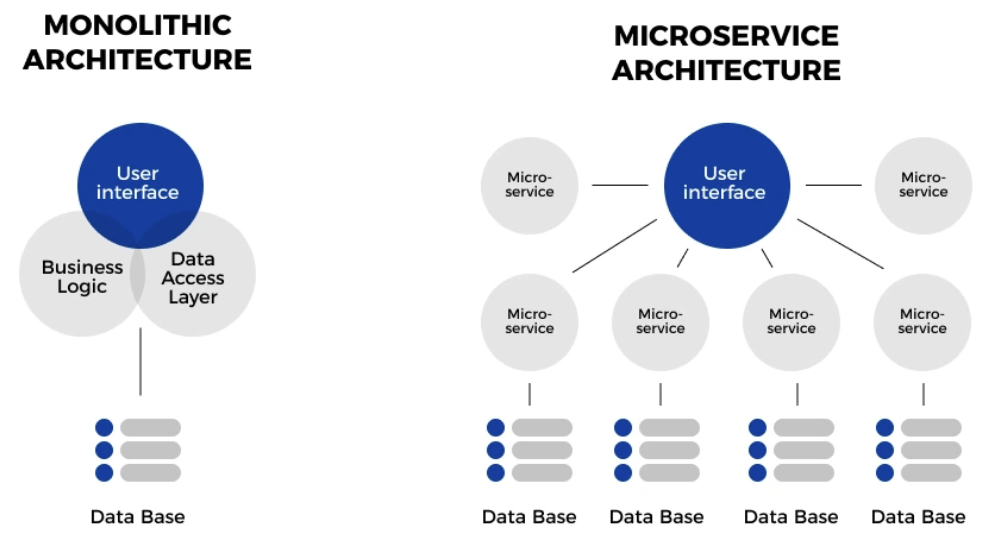
\includegraphics[width=0.7\textwidth]{Images/fundamental/micro.png}
    \vspace{12pt}\caption{Comparison of Microservice and Monolithic architecture}\label{fig:micro_vs_mono}
\end{figure}


However, as system demands grow, combining heavy processing tasks with basic web routing in a single program can cause performance bottlenecks. 
Microservices take the next step by turning logical modules into physical, independent services. Each service runs in its own process, 
often with its own separate database, and communicates with other services using standard protocols like REST APIs or message brokers.

Therefore, the Microservices architecture inherits the organizational advantages of the Modular Monolith, while providing several additional merits:
\begin{itemize}
    \item {Independent Scalability:} Microservices allow different parts of the system to scale separately. For example, a heavy processing service can be upgraded with more computing power or duplicated without needing to scale the lightweight web server. This ensures efficient hardware use during high traffic.
    
    \item {Fault Isolation:} In a microservices system, software failures are contained. If a heavy processing service crashes due to memory limits, it does not bring down the entire system. Other services, such as user login and basic web browsing, remain fully operational while the crashed service restarts.
    
    \item {Technology Flexibility:} Microservices allow developers to choose the best programming language or tool for each specific task. For instance, data science components can be built using Python for its machine learning libraries, while high-speed API routing can be written in Go or Node.js.
\end{itemize}

Alongside these benefits, Microservices possess some intrinsic disadvantages:

\begin{itemize}
    \item {Network Latency:} Internal function calls in a monolith are extremely fast. In microservices, these are replaced by network requests over the internet or local network, which inherently adds delay and processing overhead.
    \item {Operational Complexity:} Managing, monitoring, and deploying multiple independent services with separate databases is significantly harder than deploying a single program. It also requires complex strategies to keep data consistent across the entire network.
\end{itemize}

\subsection{Technology Stack and Frameworks}
The selection of frameworks is driven by the need for high-performance Python execution and seamless integration with AI libraries. These frameworks are chosen to 
building block for the implementation of the application layer, providing the necessary tools and abstractions to manage the complex interactions between the backend, frontend, and AI components. 
\subsubsection*{Backend Development}
Backend development serves as the foundational logic of any software application, responsible for data processing, security, and the orchestration of communication between the database and the client. It handles the business logic that users do not see but rely upon for functionality. For an intelligent educational system involving heavy AI workloads, the backend must be capable of handling high-concurrency requests without latency, ensuring that the complex computations of the agents do not block the user experience.
\begin{figure}[H]
    \centering
    
\includegraphics[width=0.4\textwidth]{Images/system/backend/fastapi.png}
\end{figure}
To address these requirements, we utilize FastAPI, a modern web framework for building APIs with Python. While older frameworks like Django were built on synchronous standards known as WSGI, FastAPI adopts the Asynchronous Server Gateway Interface (ASGI). This approach allows the server to handle asynchronous code natively using Python's await syntax. This represents a paradigm shift for AI applications, moving away from blocking, sequential request handling to a concurrent model where I/O-bound tasks—such as waiting for an LLM response or a database query—release the CPU to handle other incoming requests, offering some key features:
\begin{itemize}
    \item High Concurrency: By utilizing the ASGI standard, FastAPI can handle thousands of simultaneous connections (such as multiple users uploading videos or chatting with agents) without the blocking issues inherent in traditional synchronous frameworks.
    \item Data Validation: It integrates tightly with Pydantic, a data validation library. This ensures that the complex JSON outputs generated by AI agents are rigorously validated against strict schemas before being sent to the frontend, preventing runtime type errors.
    \item Performance: Built on top of Starlette, FastAPI offers execution speeds comparable to compiled languages like Go, which is critical for minimizing the latency overhead in the educational content processing pipeline.
\end{itemize}

\subsubsection*{UV: High-Performance Package Management}
Traditional Python dependency management with pip and virtualenv introduces significant overhead in complex AI projects, where dependency resolution across dozens of GPU-accelerated libraries can take several minutes. The system adopts {uv}, a Rust-based Python package manager developed by Astral, which consolidates virtual environment creation, dependency resolution, and lockfile generation into a single binary.
\begin{figure}[H]
    \centering
    
\includegraphics[width=0.4\textwidth]{Images/system/backend/uv.png}
\end{figure}
UV achieves dependency resolution 10--100 times faster than pip by implementing a custom resolver in Rust. Its deterministic lockfile mechanism ensures that all 
team members and deployment environments operate with identical dependency versions, eliminating the ``works on my machine'' class of bugs. For this project, uv manages all backend dependencies---including LangChain, LangGraph, PyTorch, and the database client libraries---providing a consistent and reproducible build pipeline from development through production deployment.
\subsubsection*{Ollama: Local Model Inference and Optimization Infrastructure}

Ollama is an advanced abstraction layer designed for managing and executing LLMs on local infrastructure. It is built upon the \texttt{llama.cpp} core, providing an efficient environment for model orchestration and hardware acceleration.
\begin{figure}[H]
    \centering
    
\includegraphics[width=0.4\textwidth]{Images/system/AI/ollama.png}
\end{figure}

A critical feature of local inference is {Quantization}, the process of reducing the precision of model weights from high-bit floating-point formats (e.g., FP16 or BF16) to lower-bit integers (e.g., 4-bit or 8-bit). This technique significantly reduces the VRAM footprint and memory bandwidth requirements:

\begin{equation}
w_{q} = \text{round}\left(\frac{w}{\Delta}\right)
\end{equation}

where $w$ is the original weight and $\Delta$ is the scaling factor. Quantization enables large-scale models to run on consumer-grade hardware with minimal degradation in perplexity and reasoning capabilities.
Moreover, it utilizes the {GGUF (GPT-Generated Unified Format)}, a binary format designed for rapid model loading and efficient metadata storage. Key technical characteristics include:
\begin{itemize}
    \item {mmap Compatibility:} Allows models to be mapped directly into memory, enabling nearly instantaneous startup times.
    \item {Unified Execution:} Supports flexible memory offloading, where layers of the model can be distributed between the GPU (VRAM) and CPU (System RAM) based on available resources.
    \item {Modelfile Abstraction:} Provides a structured way to define system prompts, temperature settings, and context window sizes within a single configuration file, ensuring deterministic behavior across different local environments.
\end{itemize}

\subsubsection*{The Langchain Ecosystem}
As mentioned in Subsction~\ref{subsub:lang_intro}, Langchain~\cite{LangChain} is a powerful framework for our educational system, with State Graph Architecture. Moreover, it is one of the first and most popular agentic 
frameworks in the industry, with a large community and rich documentation. The accumulated contributions to the ecosystem and agentic research using Langchain have provided 
us with a wealth of tools and integrations:
\begin{itemize}
    \item {Pre-built Agents:} Langchain offers a variety of pre-built agents that can be easily customized for specific use cases, such as question-answering, 
    summarization, and multi-step reasoning. In 2026, it publishes DeepAgent, capable of extremely long term reasoning and complex workflow orchestration, 
    and currently leads the harnessing researching trend in the industry.
    \item {Langfuse:} Langfuse, among with Langsmith, is one of the most powerful tools for agentic system development. It provides a comprehensive observability platform for monitoring 
    and debugging agent interactions, allowing developers to trace the decision-making process of agents in real-time. This is critical for diagnosing issues in 
    complex workflows and ensuring that the system behaves as expected, making agentic operation more transparent, manageable and less error\-prone. 
    \item {Context Management:} Langchain includes built-in context management capabilities, enabling agents to maintain context across interactions and manage state effectively.
    Those includes utilities for memory management (adapting to multiple external databases), conversation history, and dynamic context injection, which are essential 
    for building complex agentic system for long interactions over time.
\end{itemize}




\subsection{Database System Design \& Management}
Database is where you store necessary information where application can read, write, update and delete via query or integrated calls or methods. In the domain of modern software 
engineering, data handling has become increasingly complex. To address this, robust architectures utilize a Polyglot Persistence strategy, utilizing distributed 
storage technologies optimized for different data modalities.

\begin{table}[H]
    \centering
    \caption{Polyglot Persistence Architecture: Strategic allocation of storage engines.}\label{tab:polyglot_db}
    \renewcommand{\arraystretch}{1.5} % Increases row height for readability
    \small % Slightly reduces font size to fit text better
    % Defines column widths: fixed width for the first two, auto-expanding (X) for the last two
    \begin{tabularx}{\textwidth}{|p{2.0cm}|p{2.0cm}|X|X|}
    \hline
    {Storage Engine} & {Data Modality} & {System Role} & {Theoretical Justification} \\
    \hline
    Relational (MySQL) & Structured Data & User Authentication, Billing, Access Logs & Enforces ACID properties for transactional integrity and supports complex relational joins for administrative analytics. \\
    \hline
    NoSQL (MongoDB) & Semi-Structured Data & Semantic Metadata, Analysis Tags, JSON Outputs & Provides schema polymorphism to handle variable outputs from different AI agents (e.g., OCR vs. Object Detection) without sparse tables. \\
    \hline
    Object Storage (MinIO) & Unstructured Binary & Lecture Materials, Educational Assets, Audio Clips & Decouples storage from compute to prevent database bloat; utilizes Erasure Coding for high-throughput parallel streaming during ingestion. \\
    \hline
    Vector Database (Milvus) & High-Dimensional Vectors & Embeddings Index, Semantic Search & Optimized for Approximate Nearest Neighbor (ANN) algorithms (e.g., HNSW), enabling efficient similarity search in latent spaces where traditional B-Tree indexing fails. \\
    \hline
    Graph Database (Neo4j) & Multi-hop Graph Data & Knowledge Graph, Prerequisite Relationships & Optimized for traversing complex relationship networks; enables recursive queries and multi-hop reasoning to connect disparate educational concepts. \\
    \hline
    \end{tabularx}
\end{table}



\subsubsection*{Relational Database (RDBMS)}
Relational Databases are mathematically founded on Set Theory and First-Order Predicate Logic. They organize data into tuples (rows) and attributes (columns) within strictly defined relations (tables). The defining characteristic of this model is the enforcement of ACID properties (Atomicity, Consistency, Isolation, Durability), which guarantees that database transactions are processed reliably.

RDBMS is typically utilized strictly for data that requires high integrity and deterministic relationships, such as User Management and Billing. It acts as the source of truth for entity relationships, enabling complex SQL JOIN operations (e.g., selecting all learning materials uploaded by a specific role within a timeframe).
The adoption of RDBMS for core administrative data offers specific advantages to system stability.
\begin{figure}[H]
    \centering
    
\includegraphics[width=0.4\textwidth]{Images/system/database/sqlite.png}
\end{figure}

MySQL is utilized as the primary Relational Database Management System. It handles core entities such as user accounts, roles, and administrative logs, ensuring that all structured interactions follow strict relational integrity.
\begin{itemize}
    \item Transactional Integrity: In a multi-user environment where credits or permissions are updated frequently, RDBMS ensures that race conditions do not occur. For instance, if a user purchases a subscription while simultaneously uploading an educational asset, the ACID properties ensure the account balance is updated accurately before the upload permission is granted.
    \item Data Normalization: By structuring data into normalized tables (e.g., Users, Roles, Logs), redundancy is minimized. This ensures that a change in a user's details is reflected system-wide instantly, without needing to update thousands of duplicate records.
    \item Complex Querying: The robust SQL engine allows administrators to perform audit trails and analytics efficiently, such as tracking system usage patterns across different user groups, which is computationally expensive in non-relational systems.
\end{itemize}

\subsubsection*{Non-Relational Database (NoSQL)}
To address the limitations of rigid RDBMS schemas, Non-Relational databases emerged, often adhering to the CAP Theorem (Consistency, Availability, Partition Tolerance). Unlike RDBMS which prioritizes strong Consistency, NoSQL databases like MongoDB often prioritize Partition Tolerance and Availability, offering a flexible schema-less design.

Document stores are typically the primary engine for storing the Semantic Metadata derived from educational content analysis. Metadata derived from curriculum analysis is highly variable; one resource might contain OCR text, while another contains only Audio Transcripts or Face Recognition data. Document stores handle these as dynamic BSON (Binary JSON) documents, allowing fields to be added on the fly without the sparse matrices typical of rigid SQL tables.

\begin{figure}[H]
    \centering
    
\includegraphics[width=0.4\textwidth]{Images/system/database/mongodb.png}
\end{figure}
MongoDB serves as the high-performance document store for managing the semi-structured metadata generated by AI agents. It allows the system to store diverse analysis results—such as transcripts, OCR results, and agentic reasoning logs—within a single, flexible schema.
\begin{itemize}
    \item Schema Agnosticism: AI agents are constantly evolving. If an "Object Detection" agent is upgraded to output new attributes (e.g., "Confidence Score" or "Bounding Box Coordinates"), Document stores allow the new data to be saved immediately without migrating the entire database schema or breaking existing application logic.
    \item Read Performance for Aggregates: In a Knowledge-QA scenario, the system needs to retrieve the Video Title, Description, Transcripts, and Vector IDs simultaneously. In an RDBMS, this might require joining multiple tables. In a NoSQL system, this data can be stored as a single nested document, allowing the application to retrieve the entire context of a lesson in a single, high-speed read operation.
    \item Horizontal Scalability: As archives grow to thousands of hours of lecture content, metadata storage requirements increase. Native sharding capability allows data to be distributed across multiple servers economically, ensuring lookup times remain low even as the dataset grows.
\end{itemize}

\subsubsection*{High-Performance Object Storage}
While RDBMS and NoSQL excel at storing alphanumeric data, they are fundamentally inefficient for storing massive binary large objects (BLOBs) like lecture recordings, leading to database bloat and performance degradation. Object Storage systems like MinIO treat data not as a file hierarchy or a table, but as discrete objects stored in a flat address space.

High-performance architectures utilize Object Storage to handle the High Volume nature of raw educational media. It utilizes Erasure Coding—a mathematical algorithm that splits data into fragments and expands them with redundant data pieces—allowing for data recovery even if multiple drives fail. This approach decouples storage from compute; the heavy educational artifacts are offloaded to Object Storage, while the databases store only the lightweight reference pointers (URLs) to these objects.

\subsubsection{MinIO: Object Storage}
\begin{figure}[H]
    \centering
    
\includegraphics[width=0.3\textwidth]{Images/system/filestorage/minio.jpg}
\end{figure}
MinIO is deployed as a high-performance, S3-compatible object storage server. It is responsible for hosting all raw multimedia assets, including lecture videos, extracted images, and audio segments used for AI training and inference.
\begin{itemize}
    \item Decoupling Storage and Compute: By separating the raw files from the metadata databases, "database bloat" is prevented. This ensures that the RDBMS remains lightweight and responsive for user queries, while the Object Store handles the heavy I/O load of content streaming.
    \item Parallel Streaming for AI Ingestion: When an Agent analyzes a lecture recording, it requires high-speed access to the file to extract frames. Object Storage supports parallelized byte-range requests, allowing the AI to read multiple parts of a media file simultaneously. This significantly reduces the time required for the ingestion and preprocessing phase compared to reading from a standard file server.
    \item Cost-Efficiency and Redundancy: Erasure Coding allows the system to survive hardware failures without data loss, while consuming less storage space than traditional replication methods. This is vital for maintaining a massive archive of media files economically.
\end{itemize}
\subsubsection*{Vector Database}
Traditional databases are designed for structured data and are inefficient for handling high-dimensional vector data generated by AI models. Vector databases are optimized for storing and querying high-dimensional vectors, which represent the semantic content of lecture segments. They utilize Approximate Nearest Neighbor (ANN) algorithms, such as Hierarchical Navigable Small World (HNSW) graphs, to enable efficient similarity search in latent spaces where traditional indexing methods fail.

The Vector Database is the backbone of the Retrieval-Augmented Generation (RAG) paradigm, allowing the system to perform semantic search based on the embeddings generated by the AI agents. When a user query is processed, it is transformed into an embedding vector, which is then compared against the vectors stored in the database to retrieve the most semantically relevant knowledge segments.
The adoption of a Vector Database is critical for enabling the advanced retrieval capabilities required for educational analysis.

Milvus is the chosen vector database engine for SmartEdu. It indexes high-dimensional embeddings generated from course documents and lecture transcripts, providing sub-second retrieval times for semantic similarity queries across millions of vectors.
\begin{itemize}
    \item Efficient Similarity Search: Traditional databases cannot efficiently query high-dimensional vectors. Vector databases provide specialized indexing structures to handle this efficiently.
    \item Scalability for Large Datasets: As the number of educational segments grows, the vector database can scale horizontally to maintain low latency for similarity searches, ensuring that retrieval times remain fast even as the dataset expands.
    \item Integration with AI Workflows: Vector databases are designed to integrate seamlessly with AI pipelines, supporting real-time insertion and retrieval of embeddings.
    \item Support for Dynamic Data: As new educational materials are ingested and analyzed, their embeddings can be added to the vector database in real-time, allowing the system to continuously evolve and improve its retrieval capabilities without downtime.
\end{itemize}

\subsubsection*{Graph Database}
While vector databases handle semantic similarity, the structural relationships between educational concepts—such as prerequisites and curriculum hierarchies—are best modeled as a graph. 

Neo4j is utilized to store the "Backbone Graph" of the knowledge base. It represents educational entities (concepts, lessons, modules) as nodes and their pedagogical relationships as directed edges. 
\begin{itemize}
    \item Multi-hop Reasoning: Unlike relational databases that require expensive JOIN operations, Neo4j allows for efficient traversal of deep relationship chains. This is critical for detecting knowledge gaps that may span multiple prerequisite levels.
    \item Cypher Query Language: The use of Cypher enables the system to express complex pedagogical patterns, such as "Find all prerequisite concepts of concept X that the student has not yet mastered," in a readable and performant manner.
    \item Dynamic Schema: The graph model allows the knowledge structure to evolve as new educational materials are added, without needing to redefine rigid table structures.
\end{itemize}

\subsubsection*{Database Management and Observation}
Managing multiple heterogeneous database engines requires a unified observation layer to ensure data consistency and facilitate debugging during development.

DbGate is an open-source, multi-database manager used as the primary dashboard for the SmartEdu infrastructure. It provides a unified web interface to inspect and manipulate data across MySQL and MongoDB instances simultaneously.
\begin{itemize}
    \item Unified Interface: Reduces the overhead of switching between multiple specialized management tools.
    \item Schema Visualizer: Helps developers understand the evolving structure of NoSQL documents and Relational tables in real-time.
    \item Query Benchmarking: Allows for testing and optimizing complex queries before they are integrated into the application's repository layer.
\end{itemize}

\subsection{Deployment and Containerization}
Deplloyment is the process of making a software application available for real applicational usage. This section discusses the deployment strategy and the use of containerization to ensure that the system can be reliably and efficiently deployed for our AI pipeline and high\-performance stacks as discussed above.
\subsubsection*{Docker}
Docker~\cite{docker_docs} is a containerization platform that enables developers to bundle applications and their required components into isolated units called {containers}. Each container acts as a lightweight, virtualized environment that includes all the necessary elements for the application to run. Because containers are portable and consistent, they work reliably across various environments such as on-premise systems, cloud platforms, and clustered infrastructures.
\begin{itemize}
    \item {Portability:} A major advantage of Docker is its strong portability. Containers package the application together with all its dependencies, making it simple to move workloads between different environments without compatibility issues. Whether running on a local machine or a cloud server, a Docker container behaves the same way, ensuring consistency throughout the development and deployment pipeline.

    \item {Isolation:} Docker provides strong isolation between applications and their dependencies. Each container operates independently, preventing interference between applications running on the same host. This isolation enhances both security and stability, especially in shared hosting environments.

    \item {Resource Efficiency:} Docker containers are more resource-efficient than traditional virtual machines. Since containers share the same operating system kernel, they consume far less memory and disk space. This allows more applications to run on a single machine, reducing hardware overhead and simplifying resource allocation.

    \item {Scalability:} Docker supports efficient scaling of applications. By using orchestration tools such as Kubernetes or Docker Swarm, developers can easily launch multiple container instances and distribute workloads as needed. This flexibility allows systems to rapidly adjust capacity to meet varying levels of demand.

    \item {Faster Development and Deployment:} Docker improves the speed and efficiency of both development and deployment processes. Developers can work in isolated, reproducible environments identical to production, minimizing integration issues. The deployment process becomes more automated, streamlined, and less prone to errors, saving significant time.
\end{itemize}
Docker has transformed modern software development by simplifying the creation, deployment, and management of services. Its emphasis on portability, isolation, 
resource efficiency, scalability, and rapid deployment makes it an indispensable tool for both development and operations teams.

\subsection{Security: OAuth 2.0 Authorization}

OAuthis a widely used authentication and authorization protocol in backend systems across various programming languages and frameworks. Here are some general benefits of incorporating OAuth into the backend system:

\begin{itemize}
    \item {Security:} OAuth provides a secure way for users to grant third-party applications limited access to their resources without sharing their credentials. This reduces the risk of unauthorized access and protects user data.

    \item {User Experience:} OAuth enables seamless authentication and authorization experiences for users by allowing them to log in to your application using their existing accounts from trusted providers. This eliminates the need for users to create and manage yet another set of credentials.

    \item {Single Sign-On (SSO):} OAuth facilitates single sign-on capabilities, enabling users to access multiple applications and services with a single set of credentials. This improves user convenience and reduces the likelihood of password fatigue.

    \item {Granular Permissions:} OAuth allows you to define and enforce granular permissions for accessing resources. This ensures that third-party applications only have access to the specific resources they need, enhancing security and privacy.

    \item {Scalability:} By offloading user authentication and authorization to OAuth providers, your backend system can better handle scalability challenges. OAuth providers are equipped to handle large volumes of authentication requests efficiently, allowing your application to scale more effectively.

    \item {Standardization:} OAuth is a widely adopted and standardized protocol, supported by major technology companies and libraries across different programming languages. Leveraging OAuth in your backend system ensures compatibility with a broad ecosystem of tools and services.

    \item {Compliance:} OAuth implementations often come with built-in support for compliance with regulatory requirements such as GDPR (General Data Protection Regulation) or HIPAA (Health Insurance Portability and Accountability Act). This can simplify your compliance efforts and reduce legal risks.
    \item {Developer Ecosystem:} OAuth has a large and active developer community, providing extensive documentation, libraries, and support for various 
    programming languages and frameworks, such as PyJWT for protocol schema, e.t.c. This makes it easier for developers to implement OAuth in their backend 
    systems and troubleshoot any issues that may arise.
\end{itemize}

\section{Related Work}

\subsection{Document-Knowledge Modeling}
    Converting documents into structured knowledge representations has become a critical task for so long in the industry and education specifically. To replace manual 
curation in educational contexts, which is time-consuming and not scalable, prior attempts have been focusing on the power of entity extraction, prerequisite relation 
reasoning, and RAG. This has been indeed a fine strategy, given the success of early supervised models like \texttt{PREREQ}~\cite{PREREQ} using latent topic 
representations with Siamese networks to infer course dependencies, which achieved over 70 \% Precision@100 scores on the \texttt{University Course} 
and \texttt{NPTEL MOOC datasets}. However, the traditional methods of entity extraction and relation reasoning often rely on rule-based systems or pure statistical machine learning techniques, 
which can struggle to capture the complexity and nuance of educational content's relationships. Moreover, recent researches~\cite{weller2025theoretical,LostInTheMiddle} have proven that models 
fail drastically to access relevant information when documents exceed a certain length. That is the reason why though prior researches gained impressive results on medium retrieval benchmarks, 
they are not easily applied in industry when it comes to massive and unstructured enterprise data.
\begin{figure}[H]
    \centering
    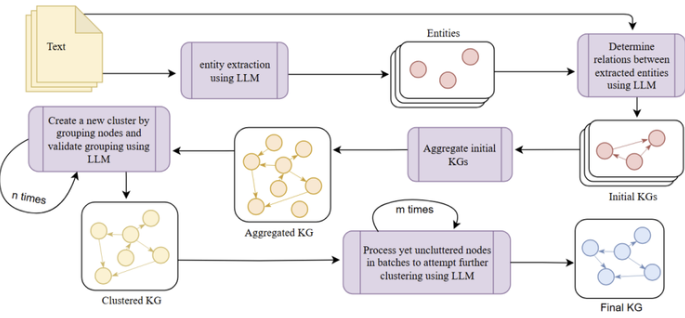
\includegraphics[width=0.8\textwidth]{Images/relate/kggen.png}
    \vspace{12pt}\caption{KGGen with multiturn LLM reasoning, grouping generation}\label{fig:kggen}
\end{figure}
    To address this, LLM-based frameworks have been widely proposed. A prime example is \texttt{KGGen}~\cite{KGGen}, an automated system that utilizes a 
clustering algorithm to group synonymous entities and relations, resulting in denser and better-connected graphs that scored an impressive 81.03\% average 
fact accuracy on the \texttt{MINE-2} (Measure of Information in Nodes and Edges) benchmark. The \texttt{EDC}~\cite{EDC} framework extends this capability by 
extracting, automatically defining schemas, and canonicalizing knowledge triples without predefined schemas, consistently surpassing state-of-the-art baselines on 
complex datasets like \texttt{WebNLG}, \texttt{REBEL}, and \texttt{Wiki-NRE}. 
\begin{figure}[H]
    \centering
    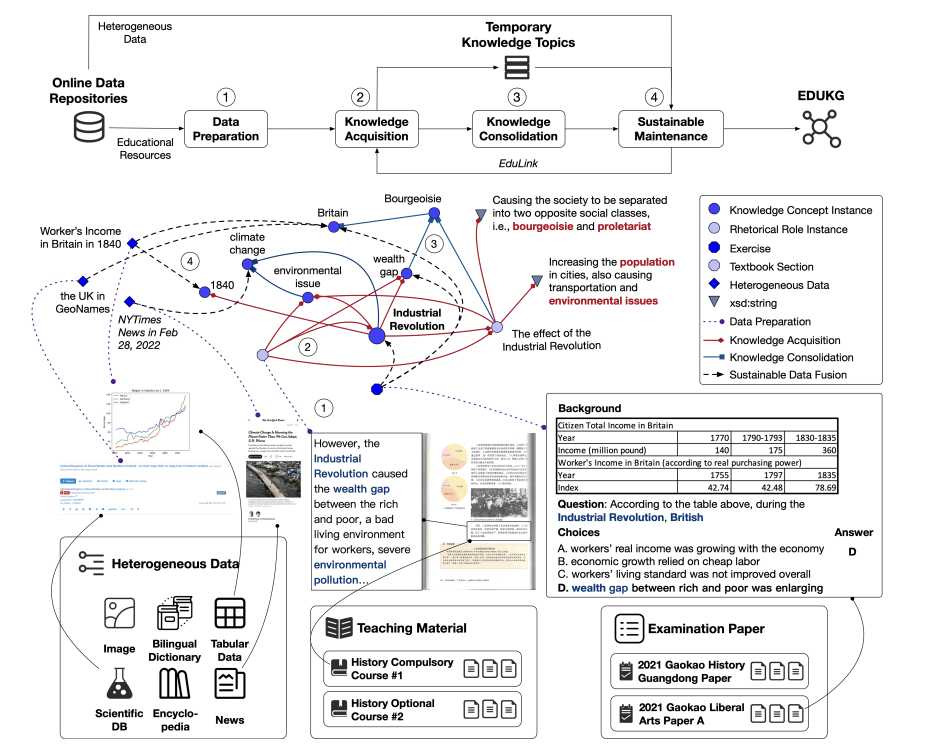
\includegraphics[width=0.8\textwidth]{Images/relate/edukg.png}
    \vspace{12pt}\caption{The end-to-end EduKGPipeline framework for educational knowledge construction and retrieval.}\label{fig:edukgpipeline}
\end{figure}
    However, LLMs have deadly drawbacks. First and most popular of all is the "hallucinations problem" leading to inaccurate, destructurized extractions. To mitigate this, \texttt{GraphJudge}~\cite{GraphJudge} proposes using a fine-tuned open-source LLM as a "judge" to score and filter out incorrect 
knowledge triples generated by naive LLMs. Validated on general (\texttt{REBEL-Sub}, \texttt{GenWiki}) and domain-specific benchmarks (\texttt{SCIERC}, 
\texttt{Re-DocRED}), it achieved over 90\% judgement accuracy. Furthermore, for large-scale educational and enterprise systems requiring cost and latency 
optimization, comprehensive hybrid pipelines have proven highly effective in practices. For instance, \texttt{EduKGPipeline}~\cite{EduKGPipe} establishes 
an end-to-end framework fusing traditional text extraction with transformer-based weighting, demonstrating high precision on educational transcripts from the 
\texttt{CCI dataset}. 
\begin{figure}[H]
    \centering
    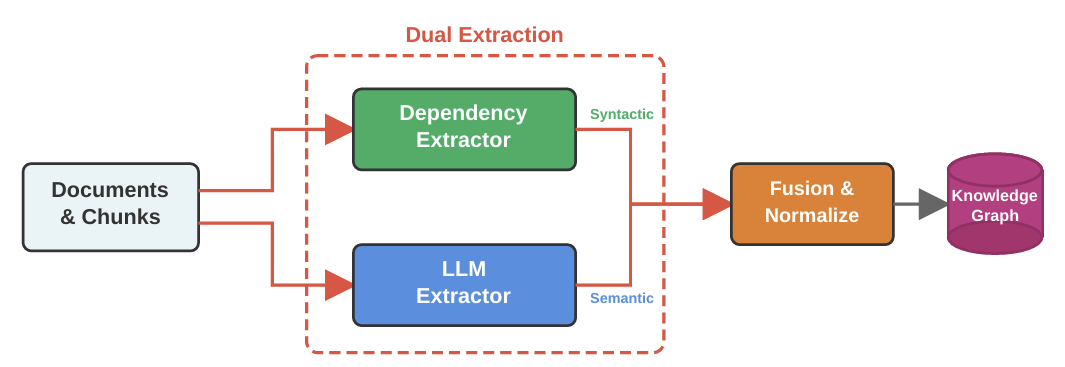
\includegraphics[width=0.8\textwidth]{Images/relate/graphrag hybrid.png}
    \vspace{12pt}\caption{Hybrid architecture of GraphRAG allow minimal cost and guarantee alignment of generated to original context}\label{fig:graph_hybrid}
\end{figure}
Similarly, recent efficient GraphRAG architectures~\cite{GraphRAG} substitute expensive LLM extractions with classical dependency parsing 
to maintain scalability, retaining 94\% of LLM-based performance on \texttt{RAGAS} metrics when evaluated on real-world enterprise datasets like \texttt{CCM} 
(Custom Code Migration). Finally, \texttt{CoDe-KG}~\cite{CoDeKG} utilizes syntactic decomposition to process complex sentences, thereby significantly enhancing 
information recall by an 8-point gain on rare relations across the \texttt{REBEL} and \texttt{WebNLG2} benchmarks.

Another inevitable error lies in the LLMs' limited context length, making it unable to generalize broad knowledge. It is good when discovering short-dependent 
context/entities/relationships in small sections but 
fails for long dependencies of extremely long documents and course information. Trying to inject an excessive amount of information even when cut by windows, 
until now with the current level, only leads to redundant costs from multiple calls, information overload, and decreased accuracy. To uncover hidden relationships 
and deduce learning paths beyond textual information, some studies shifted to an algorithmic approach.
\begin{figure}[H]
    \centering
    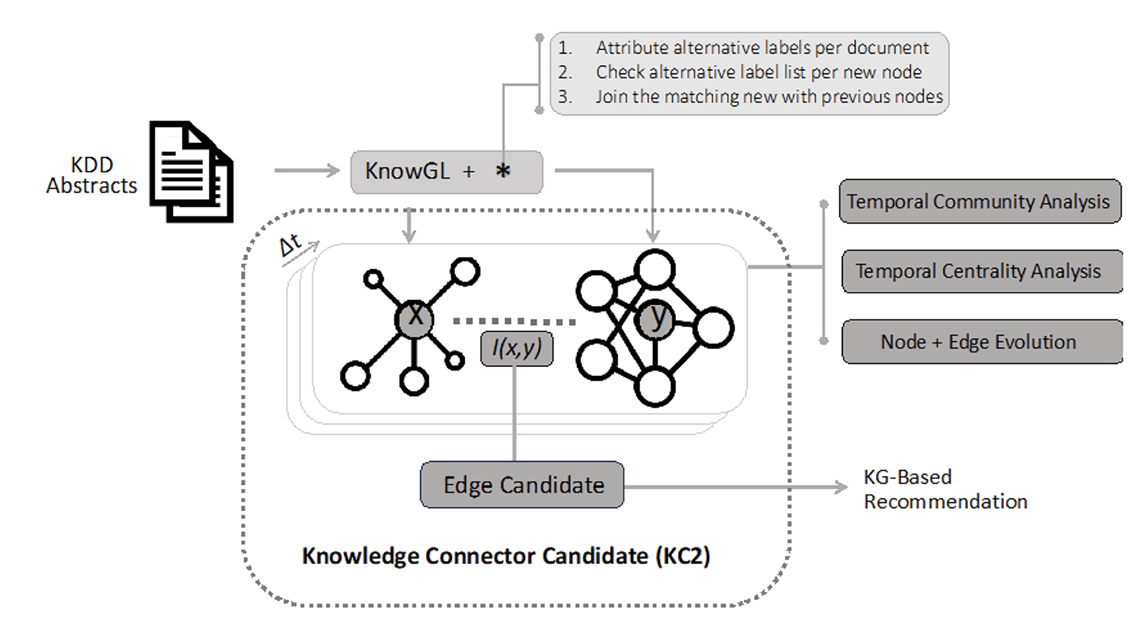
\includegraphics[width=0.8\textwidth]{Images/relate/dkg.png}
    \vspace{12pt}\caption{Dynamic Knowledge Graph (DKG) approach tracking knowledge evolution over time.}\label{fig:dkg}
\end{figure}
The \texttt{Dynamic Knowledge Graph (DKG)}~\cite{DKG} is one of the strongest representative to this approach, analyzing Knowledge Graph's macroscopic structure. To recommend strong relational paths, DKG introduces the \texttt{KC2 (Knowledge Connector Candidate)} algorithm, which uses closeness 
centrality to suggest connections between disconnected knowledge islands. Additionally, to cluster knowledge into logical chapters or modules, the 
\texttt{Leiden}~\cite{Leiden} algorithm is utilized to optimize the CPM quality function, ensuring that knowledge communities are absolutely well-connected 
and not disjointed—a common flaw of the traditional Louvain algorithm. It also divides KGs into discrete time snapshots and applies network science to track 
knowledge evolution and clustering group changes, creating a dynamic regroup, reformulation of clusters and formulation of new knowledge groups.

\subsection{Generative AI in Interactive Teaching}
Bridging the gap between raw document extraction algorithms and end-user educational platforms is the integration of Generative AI and Large Language Models (LLMs). 
The increasing accessibility and reasoning capabilities of Generative AI tools have led to widespread exploration in educational settings, fundamentally 
transforming traditional teaching and learning paradigms~\cite{AI_in_Edu}. Modern LLM agents are proved to be capable of autonomous reasoning, 
tool manipulation, and orchestrating complex academic tasks. 

\subsubsection*{Advances in Educational Agents}
Recent surveys highlight the versatility of LLM agents in automating multifaceted educational workflows, ranging from curriculum design to generating highly contextualized 
feedback~\cite{llm_in_edu}. These agents operate dynamically, leveraging multi-hop reasoning and continuous interaction to adapt to a student's cognitive state. A qualitative study involving educators demonstrated that the core impact of generative models spans three critical pillars: active teaching and learning, administrative automation, and personalized assessments~\cite{AI_in_Edu}. 

A prominent, large-scale empirical example of this shift is the integration of AI within Harvard University's CS50 course. By deploying a suite of specialized 
AI-based software, the course successfully approximated a 1:1 teacher-to-student ratio. Crucially, the system was designed with pedagogical boundaries—guiding 
students toward conceptual understanding rather than merely offering outright code solutions. This constrained autonomy proved highly effective in code explanation, 
style improvement, and administrative querying, demonstrating the practical viability of AI as a ubiquitous teaching assistant~\cite{ai_4_CS50}.

\subsubsection*{Challenges and Deployment Bottlenecks}
Despite the profound opportunities, deploying LLM agents in educational ecosystems introduces substantial systemic and ethical challenges. The inherent probabilistic 
nature of LLMs frequently leads to "hallucinations," where the model confidently generates factually incorrect or pedagogically flawed information. Furthermore, 
there is a significant risk of cognitive offloading, where students develop an overreliance on AI, thereby degrading their independent problem-solving 
skills~\cite{llm_in_edu}. 

From a practitioner's perspective, integrating these models into open-source or institutional infrastructure often encounters severe operational bottlenecks. 
Empirical analyses of LLM-based open-source projects categorize these challenges primarily into model configuration issues, connection instabilities, and feature 
misalignment, all of which hinder seamless deployment~\cite{open_source_isue}. Furthermore, theoretical analyses of LLM representations reveal phenomena such as 
"semantic collapse," where the continuous manifold of the model's activations struggles to maintain stable, logically sound ontologies over continuous, long-term 
reasoning tasks without rigid architectural constraints~\cite{semantic_collapse}. These limitations emphasize the need for robust frameworks to 
tightly navigate the semantic boundaries for AI agents in an academic context.

\subsubsection*{Agentic Workflows}
As educational AI transitions from static next-token prediction to autonomous multi-agent collaboration, ensuring the reliability, alignment, and transparency of 
these systems becomes a critical engineering challenge. Traditional benchmarks, which typically evaluate single-response accuracy, are inadequate for assessing the 
non-linear, multi-step nature of agentic workflows. 

This necessitates the development of rigorous, process-aware evaluation frameworks. Architectures like the Adaptive Evaluation Multi-Agent (AEMA) framework have been 
proposed to address this gap. AEMA provides an auditable, multi-step evaluation mechanism that operates under human oversight, ensuring that the agents' internal 
decision-making processes, tool selections, and collaborative strategies are verifiable and transparent~\cite{AEMA_agentic_eval}. Implementing such verifiable 
frameworks is essential to mitigate the risks of unconstrained autonomy, ensuring that the integration of AI into education remains both trustworthy and pedagogically effective.

\subsection{Educational Intelligent System}
Smart AI based educational systems has leverage from pure research topic and find itself introduced to commercial use. A lot of Intelligent commercial platforms have been 
born recently, and research instituitions have also propose a fully end-to-end pipeline beyond a benchmarked study method. 

In research field,~\cite{EduKG} (along with variants like K12EduKG and MOOC-KG) has been developed to uniformly model knowledge from textbooks and online courses. The~\cite{EduKGPipe} framework automates KG construction from unstructured PDF documents by extracting keywords via Keybert and performing semantic linking with LLMs. 
Furthermore, \texttt{MEduKG} pushes beyond text limitations by integrating multi-modal data into the graph, thereby enhancing the system's comprehensiveness and 
vividness for students.

As mentioned, some systems relating to this field have also reached the market. Popular platforms worldwide like \texttt{Khanmigo} leverage 
Generative LLMs to provide personalized tutoring and real-time feedback, with enormous available resources.
For Vietnamese representative, \texttt{VioEdu} utilizes a manually curated knowledge tree to structure its curriculum, while 
\texttt{EdMicro}, specialized for enterprises, employs a skill matrix to map out learning objectives and prerequisites. 
 These systems represent different approaches to integrating AI into education, each with its own strengths and limitations in terms of scalability, personalization, and content structuring.
Based on practical surveys and evaluation criteria, current educational systems in the market exhibit various characteristics regarding AI and knowledge structuring. A comparative analysis of these platforms is presented in Table \ref{tab:edu_sys}.

\begin{table}[H]
\centering
\resizebox{\textwidth}{!}{
\renewcommand{\arraystretch}{1.4}
\begin{tabular}{|p{8.0 cm}|c|c|c|c|c|}
\hline
\textbf{Criteria} & \textbf{EduKG} & \textbf{Khan Academy} & \textbf{Docebo} & \textbf{VioEdu (FPT)} & \textbf{EdMicro} \\
\hline
\textbf{Adaptive learning:} Personalize the learning process based on needs, abilities, and preferences. & High & High & Low & Medium & Medium \\
\hline
\textbf{Intelligent Recommendations:} Some personalized suggestions courses, videos based on preferences, and areas of improvement. & High & High &  & Low &  \\
\hline
\textbf{Natural language processing for queries:} Based on the questions from learners, it can give out the answer based on the content the LMS has in its DATABASE. & High & Medium & & & \\
\hline
\textbf{Learning analytics/Progress Tracking:} AI-based analytics track and analyze user progress. Can visualize using tracking board, and leaderboard. & Medium & High & High & High & High \\
\hline
\textbf{Text-to-audio content:} Provide audios for text content. & & High & & & \\
\hline
\textbf{Interactive learning method:} Interactive content, such as quizzes, coding exercises, and simulations, can engage learners and reinforce learning. & Low & Low & Medium & Medium & Medium \\
\hline
\textbf{Dynamic KG Reasoning \& Roadmap:} Automatically extract concepts and mathematically reason long-term prerequisite learning paths without manual expert input. & & & & & \\
\hline
\end{tabular}
}
\caption{Comparative analysis of representative educational intelligent systems based on key AI and knowledge features.}\label{tab:edu_sys}
\end{table}

\subsection{Conclusion and Research Gaps}\label{sub:gaps}
During the survey of mentioned representative researches, upon studying from multiple peer reviews and self-reviews of those, this report pinpoints the following core 
research gaps in the current landscape:

\paragraph*{{Limitations in Automation and Cost Optimization:}} All mentioned big systems heavily depend on manually built knowledge trees or skill matrices. Course contents, 
structured and ordered by expertise indexing, but lack inner modelling and semantic makes the system less adaptive to students' needs and preferences, 
leading to good courses recommendations but terrible inner course concept recommendations.
This makes learning path become a linear process and not flexible on the micro scale, with little to no revision and update. 
The lack of automation also limits the scalability of these systems, as manual labeling becomes increasingly impractical as the amount of content grows.
\paragraph*{{Lack of Connectivity and Transparency in Lesson Structures:}} Traditional methods like clustering in text-mining often produce disconnected 
or fragmented knowledge groups. Existing learning platforms typically lack a standard, mathematically proven network algorithm for dividing study modules, leading 
to disjointed learning path that disrupt the learners' cognitive flow.
    
\paragraph*{{Static Roadmap Reasoning and Gap Detection:}} While current LMSs and AI tutors provide generated advice, they are actually still relied on traditional long 
form docs or RAG, lacking the network structure and deterministic approach to map out prerequisites dynamically. The identification of critical "knowledge gaps" remains 
static and reactive, failing to automatically trace back to the fundamental bridge concepts (based on network centrality) that cause student bottlenecks.

So far~\cite{EduKGPipe} and its lineages have made a significant attempt to propose solutions to those mentioned problems with an 
end-to-end pipeline that fuses traditional text extraction with transformer-based weighting.~\cite{DKG} has proposed what~\cite{EduKGPipe} is missing: a mathematical 
efficient community detection method, furthermore solve the connectivity and transparency issues in lesson structures that almost all of previous pipeline encountered. 
However both have their own limitations. The former has no deterministic knowledge mapping, which causes knowledge disruption (even when the graph is not fragmented), 
while the latter pipeline is not as efficient in multistep extraction as the former, thus good for knowledge modeling and analysis but not inference and recommendation. 
Finally, a lot of great proposal here are not widely adapted due to the lack of a comprehensive system that make use of their research project. 


\newpage
\chapter{Requirements Specifications}\label{chap:req}

The limitations discussed in Subsection~\ref{sub:gaps} have shaped the technical vision for the proposed system. To address these gaps and deliver a robust, 
scalable educational platform following our goal (Section~\ref{sec:goal}), this section outlines the explicit Functional and Non-Functional Requirements, as well as 
visiallizing use---case design. These requirements are derived directly from the systemic constraints and the pedagogical needs of learners for a more personalized, 
diversed and comprehensive learning assistance system.

\section{Functional Requirements}

\subsection{Knowledge Modelling and Management}
As a key objective feature, knowledge modelling construct knowledge base, foundation to all other key features. This functional category encompasses the capabilities 
required to process raw educational inputs into a structured knowledge base.

\begin{itemize}
    \item \textbf{Data Ingestion and Parsing:} 
    \begin{itemize}
        \item The system must be able to ingest unstructured, text-dense academic formats (e.g., PDF textbooks, syllabus guidelines).
        \item The system must accurately parse text into discrete chunks while retaining crucial positional metadata (e.g., source file origin, exact page numbers).
    \end{itemize}
    
    \item \textbf{Semantic Extraction and Normalization:}
    \begin{itemize}
        \item The system must extract fundamental educational concepts and their explicit pedagogical relationships from the ingested text.
        \item The system must normalize extracted entities to a canonical form to ensure conceptual consistency and prevent any form of semantic fragmentation (even of different course) 
        across the knowledge base.
    \end{itemize}
    
    \item \textbf{Hierarchical and Relational Organization:}
    \begin{itemize}
        \item The system must organize extracted entities into a standardized hierarchical topology.
        \item The system must automatically group highly related concepts into cohesive educational clusters or chapters.
        \item The system must explicitly define and store directional "prerequisite" relationships between concepts to enable automated learning path generation.
    \end{itemize}
    
    \item \textbf{Storage Capability:}
    \begin{itemize}
        \item The persistence mechanism must guarantee a database structure that facilitates high-speed, complex relational querying and subgraph retrieval during live 
        interactions.
        \item To ensure diversity of learning input, storage design must ensure efficient storing of enormous data with reasonable latency. 
    \end{itemize}
\end{itemize}

\subsection{Intelligent Teaching Assistance}
To utilized modeled knowledge base as well as guarantee satisfactory learning experience and result, the design of agentic system that serves as our Teaching Assistance 
is crucial. This category defines the required behaviors and reasoning capabilities of the automated teaching assistant.

\begin{itemize}
    \item \textbf{Intent Recognition and Context Orchestration:}
    \begin{itemize}
        \item The system must classify user intents (e.g., Retrieve information, Generate roadmap, Clarify concepts) and autonomously route the request to the appropriate internal workflow.
        \item The system must dynamically gather necessary context before responding, which includes retrieving the student's personal mastery history and the relevant subset of the educational knowledge base.
    \end{itemize}
    
    \item \textbf{Intelligent Reasoning and Supervision:}
    \begin{itemize}
        \item The system must support a Socratic teaching interaction; it must be capable of generating probing questions to assess student comprehension 
        rather than merely providing direct answers.
        \item The system must objectively evaluate the student's response to determine whether to authorize progression to the next prerequisite topic.
        \item The system must be able to autonomously detect when it lacks sufficient context to answer a question and execute a fallback strategy that 
        synthesizes information from the broader knowledge base.
    \end{itemize}
    
    \item \textbf{Response Verifiability and Fallback:}
    \begin{itemize}
        \item To guarantee grounded responses, the system must prioritize explicit document referencing, citing exact source pages for its generated answers.
        \item The system must execute a broader knowledge synthesis fallback only when direct contextual concepts are missing from the immediate document.
    \end{itemize}
\end{itemize}

\subsection{Student Interaction and System Navigation}
This category defines the functional requirements concerning the end-user's experience, accessibility, and direct interaction with the intelligent system.

\begin{itemize}
    \item \textbf{Identity and Access Security:}
    \begin{itemize}
        \item The system must provide secure authentication capabilities (Login/Logout) to uniquely identify users.
        \item The system must maintain isolated, tamper-proof session states for each user to securely record individual learning progress without cross-user data exposure.
    \end{itemize}
    
    \item \textbf{Interactive Dialogue and Visualization:}
    \begin{itemize}
        \item The system must provide a natural language chat interface that supports continuous, multi-turn conversational interactions and real-time streaming responses.
        \item The system must dynamically render visual learning roadmaps, empowering students to make informed, user-centric choices regarding their educational progression rather than following a static curriculum.
        \item The interface must consolidate essential learning tools, providing seamlessly integrated functional components such as conversational history logs, a synchronized document viewer, and progress summarization dashboards.
    \end{itemize}
    
    \item \textbf{Advanced Navigation and Content Discovery:}
    \begin{itemize}
        \item The system must implement an intuitive, multi-level navigation structure (e.g., breadcrumb trails) to help students orient themselves within complex knowledge hierarchies.
        \item The system must incorporate a powerful semantic search utility, allowing users to rapidly query and locate specific educational materials, graph concepts, or historical interactions.
    \end{itemize}
    
    \item \textbf{Contextual and Responsive Feedback:}
    \begin{itemize}
        \item The system must be capable of emitting explicit interface triggers alongside its textual responses to automatically synchronize the user's interface (e.g., auto-scrolling the document viewer to the exact referenced page).
        \item Notifications and intelligent pedagogical prompts must be delivered in a non-intrusive, accessible manner that captures user attention while preserving the fluidity of the learning experience.
    \end{itemize}
\end{itemize}


\section{Non-Functional Requirements}
To create a powerful, reliable, and user-friendly educational platform, the Smart Learning System cannot stop at being functional, but need focusing on efficiency 
and overall system performance. Thus, it must also adhere to a set of non-functional requirements that govern its 
performance, scalability, security, and overall user experience.
\begin{itemize}
    \item \textbf{Scalability and Modularity:}
    \begin{itemize}
        \item The backend architecture must be designed as stateless, relying exclusively on external persistence layers for state management to ensure readiness 
        for future distributed scaling.
        \item System design must be modular, with clear separation of components reponsibility and dependency to facilitate future enhancements, maintenance, and potential integration of 
        additional features or third-party services.
    \end{itemize}

    \item \textbf{Resource Optimization and Latency Minimization:}
    \begin{itemize}
        \item Operating under the constraint of localized execution, the system must optimize memory and computational overhead, loading resource-heavy 
        models into memory only when explicitly demanded by an active workflow.
        \item All resource must be efficiently released immediately after use to minimize the system's memory footprint and ensure responsiveness.
        \item System must be scheduled to be constantly running, minimizing downtime and waiting time for any task.
        \item All resource must be managable, specifically for developers and system administrators, but crucial for maintaining system stability and performance.
    \end{itemize}

    \item \textbf{Reliability and Determinism:}
    \begin{itemize}
        \item The system must mitigate the inherent unpredictability of generative AI by enforcing strict, programmatic data schemas for all internal system communications and decision-making logic.
        \item Complex analytical tasks, such as calculating knowledge gaps, must be executed via deterministic programmatic logic rather than relying on probabilistic generative approximations.
    \end{itemize}

    \item \textbf{Observability and Traceability:}
    \begin{itemize}
        \item The system must maintain comprehensive telemetry across all automated workflows.
        \item Database state changes, including knowledge graph updates and student progress logs, must be monitored and saved to enable historical analysis and rollback capabilities.        
        \item Every automated decision, context retrieval action, and resource consumption metric must be actively logged to provide a transparent audit trail for both system debugging and pedagogical evaluation.
    \end{itemize}
    \item \textbf{User Experience and Interface Requirements:}
    \begin{itemize}
        \item User interface is focus on the simplicity and intuitiveness, ensuring that users of varying technical proficiency can navigate the system effectively.
        \item User interface must be responsive and accessible, adhering to modern web standards to ensure compatibility across a wide range of devices and screen sizes (phones, tablets, desktops).
        \item Client side shouldn't be pulled by heavy backend response latency. It should maintain a fluid, real-time interaction experience, minimizing latency 
        in response generation and interface updates. Mininizing \texttt{"user experience latency"} regardless of system performance 
        is a strategic design move to preserve conversational engagement as well as learning interest.
    \end{itemize}

\end{itemize}



\newpage
\chapter{Proposed Methodology and Paradigm}\label{chap:methodology}
Founded on the vision outlined in the requirements specification (Chapter~\ref{chap:req}), this research aims to propose a novel system that combines the strengths of 
classical Graph-based architectures with the generative capabilities of Large Language Models (LLMs). This chapter details the foundational methodology of our system. 
\section{Overview}
The proposed paradigm can be construcuted and visualized as the below pipeline
\begin{figure}[H]
    \centering
    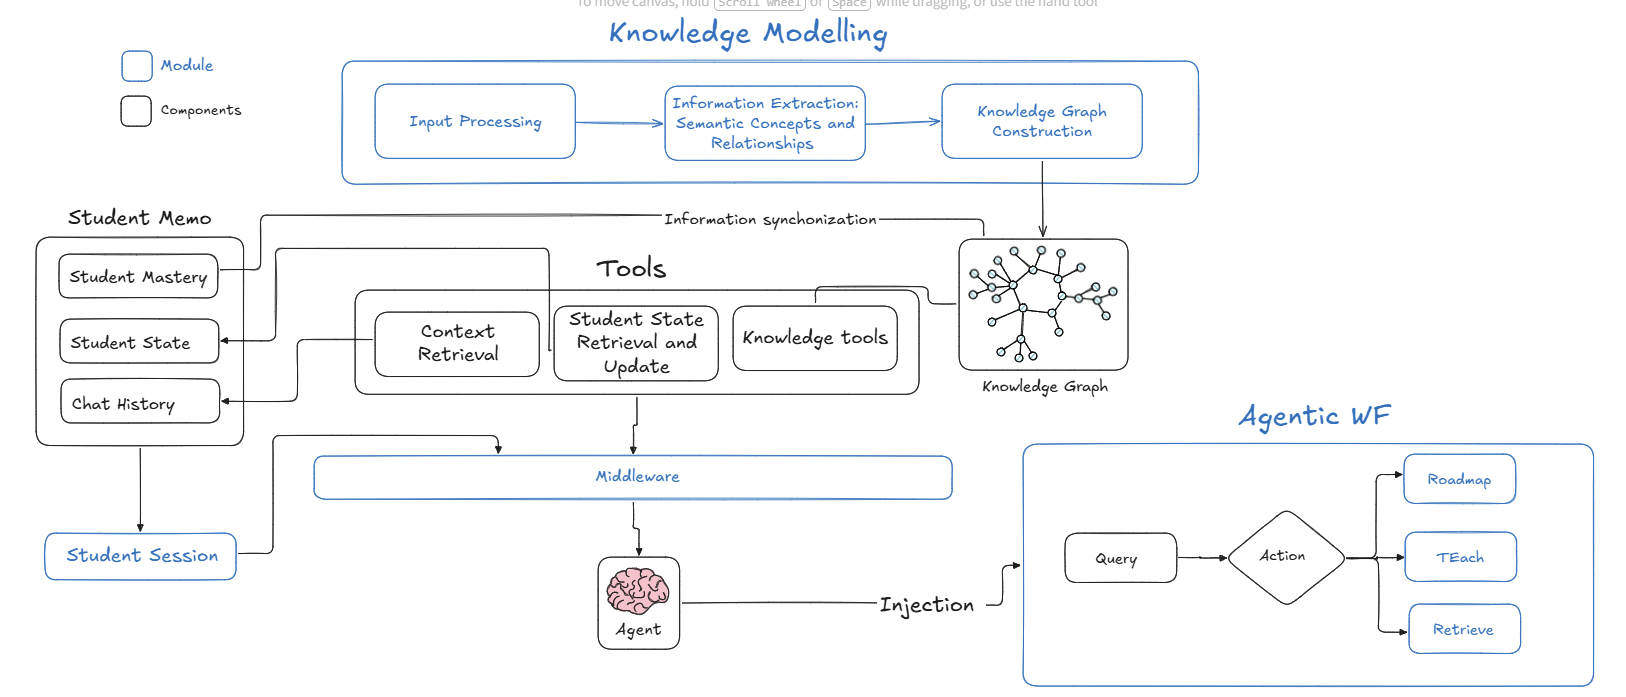
\includegraphics[width=\textwidth]{Images/method/pipeline.png}
    \vspace{12pt}\caption{High level visualization of how the system should work}\label{fig:macro_workflow}
\end{figure}

A key security boundary is established at the system's entry point. Upon user authentication, the student's Session and Memo contexts are directly injected into the 
computational tools. As a result, the agents use these pre-configured tools instead of interacting directly with the database. This approach ensures strict data 
isolation and prevents the LLM from making unauthorized or destructive database transactions.

\section{Knowledge Modelling: Educational Graph}
This section proposes a hybrid methodology that anchors the generative flexibility of LLMs to the deterministic rigor of Graph Construction and Natural Language Processing. 
By formulating the educational domain as a Property Graph, the proposed system (SmartEdu) achieves a necessary synthesis of semantic richness and logical consistency, 
overcoming the unstructured chaos often associated with pure generative models.
\subsection{Graph Definition}\label{sub:g_def}
To construct a graph, we need to define and regulate it with a connected, rigorous structure. Simulating educational concepts, the graph contains ontologies as well as 
topic's relationship like presiquite. The subsequence contents in this subsection explain the deterministic algebra representation and rules explanation of it.
\subsubsection{Formal Property and Topological Definition}

To accurately represent the vast, interconnected semantic structure inherent in educational curricula, our methodology employs a formal Property Graph formulation. Unlike simple directed graphs, a property graph allows both vertices and edges to possess complex internal states (properties). This multidimensionality is highly suitable for educational knowledge representation, where a concept is not just a node, but a container of definitions, mathematical formulas, and historical context.

We define the Educational Knowledge Graph (EKG) as a heterogeneous, directed property graph, formally denoted as:
\begin{equation}
    G = (V, E, \Lambda, \Pi)
\end{equation}
where:
\begin{itemize}
    \item $V$ is the set of vertices (nodes), representing distinct educational entities spanning multiple levels of abstraction.
    \item $E \subseteq V \times V$ is the set of directed edges, representing the semantic and structural relationships between entities.
    \item $\Lambda$ is a finite, predefined set of labels, acting as ontological categories that strictly classify the nodes to prevent semantic drift.
    \item $\Pi$ is a set of properties, expressed as key-value pairs $\pi_{key} = value$, associated with both nodes and edges to store metadata, raw textual content, and dynamically updated quantitative metrics.
\end{itemize}

The necessity of this mathematical definition lies in its ability to enforce data integrity. By treating the knowledge base as a set $V$ and a mapping $E$, we can apply rigorous graph-theoretic algorithms (such as topological sorting and shortest-path routing) directly to the curriculum, effectively translating human pedagogical intuition into computationally solvable problems.

\subsubsection{Ontological Hierarchy formulation}

To accurately model the multi-scalar nature of educational curricula—ranging from entire academic disciplines down to specific explanatory sentences in a textbook—we artificially constrain the label set $\Lambda$ such that $\Lambda = \{ \text{CommunityNode}, \text{TopicNode}, \text{ConceptNode}, \text{RhetoricalNode} \}$. This rigorous ontological taxonomy ensures structural consistency across different domains:

\begin{itemize}
    \item {CommunityNode}: Represents the highest level of educational aggregation. It functions as the macroscopic backbone of a course or a major disciplinary cluster, grouping broad fields of study (e.g., "Computer Science", "Artificial Intelligence").
    \item {TopicNode}: Represents a specific subject matter, module, or chapter nested strictly within a parent community (e.g., "Machine Learning", "Neural Networks").
    \item {ConceptNode}: The atomic unit of educational instruction. It represents distinct, indivisible ideas, theories, algorithms, or historical events (e.g., "Backpropagation", "Decision Tree").
    \item {RhetoricalNode}: Encapsulates the instructional function of the raw text. It contains specific properties $\pi_{rrole} \in \Pi$ that designate the rhetorical role of the information (e.g.,  {Definition},  {Application},  {Statement},  {Theorem}). This allows the system to distinguish between *what* a concept is and *how* it is explained.
\end{itemize}

By enforcing this strict hierarchy, the system prevents the "flattening" of knowledge, ensuring that the AI agent can distinguish between a broad topic that requires a multi-week syllabus and a specific concept that can be explained in a single paragraph.

\subsubsection{Edge Semantics and Constraints}

The topological structure of $G$ is governed by the relation types assigned to the edges $e \in E$, formulated as ordered pairs $e = (v_i, v_j, \lambda_e)$, where $\lambda_e$ is the edge type. The system defines several core edge types to represent real-world pedagogical connections: $ {PART\_OF}$, $ {RELATED\_TO}$, and $ {PREREQUISITE\_OF}$.

The mathematical enforcement of the $ {PREREQUISITE\_OF}$ edge is of paramount educational importance. In human learning, knowledge is inherently sequential; one cannot grasp Calculus without first mastering Algebra. To ensure logical learning progressions computationally, the sub-graph induced by all $ {PREREQUISITE\_OF}$ edges must strictly form a {Directed Acyclic Graph (DAG)}. 

Let $G_{prereq} = (V, E_{prereq})$ where $E_{prereq} = \{ e \in E \mid \lambda_e =  {PREREQUISITE\_OF} \}$. The methodology mandates that no directed cycles exist within $G_{prereq}$:
\begin{equation}
    \forall v \in V, \nexists \text{ path } P = (v, \dots, v) \text{ in } G_{prereq}
\end{equation}

This acyclic constraint is not merely a theoretical preference; it is a foundational mathematical requirement. If a cycle were to exist (e.g., A is a prerequisite for B, 
B is a prerequisite for C, and C is a prerequisite for A), the student would be permanently trapped in a circular dependency, unable to begin learning any of the 
concepts. Enforcing the DAG constraint guarantees that algorithms like Topological Sorting can be successfully applied 
to generate optimal, conflict-free learning roadmaps.

\subsection{Graph Construction}

A major challenge in building an automated knowledge base is extracting structured relationships from unstructured educational text. Single-pass LLM extractions—where 
the model tries to identify concepts, classify them, and link them all at once-are extremely prone to failure. Multiple frameworks propose multi\-turn LLM synthesis, but 
costly and still not guarantee a solid, hallucination immunity graph as subsequence turns increase entropy and the context total amount. I propose a hybrid method of Dual LLM extraction combining with NLP based filtering and normalization,
guarantee a consistent graph.
\subsubsection{Input Ingestion}\label{subsub:sliding}

Before the dual-phase extraction pipeline can operate, raw educational documents must be segmented into manageable batches that respect both the language model's context budget and the semantic continuity of the source material. The system employs an overlapping sliding window strategy that partitions each document into consecutive page batches with deliberate redundancy at their boundaries.

The process begins with a document parser that converts each PDF into a sequence of page-indexed text blocks, filtering out non-informational 
elements such as lecturer contact details, rendering artifacts, and fragments shorter than five characters. The resulting pages are then grouped 
into fixed-width batches: fifteen pages per batch for lecture slides and ten pages for textbooks (By default). These widths are calibrated to remain within the 
extraction model's context capacity.

Rather than advancing the window by its full width, the system steps forward by approximately two thirds of the window size, leaving an overlap of several pages 
shared between consecutive batches. For instance, a fifteen-page window advances by eleven pages, so each pair of adjacent batches shares four pages of content at 
their boundary.

\begin{figure}[H]
\centering
\begin{tikzpicture}
  % Batch 1
  \fill[blue!20, rounded corners=2pt] (0,0) rectangle (7.5,0.6);
  \node[font=\small] at (3.75,0.3) {Batch 1 (pages 1--15)};
  
  % Batch 2
  \fill[red!15, rounded corners=2pt] (5.5,-0.9) rectangle (13,-0.3);
  \node[font=\small] at (9.25,-0.6) {Batch 2 (pages 12--26)};
  
  % Overlap zone
  \fill[purple!25, rounded corners=2pt] (5.5,0) rectangle (7.5,0.6);
  \fill[purple!25, rounded corners=2pt] (5.5,-0.9) rectangle (7.5,-0.3);
  
  % Overlap label
  \draw[purple!60, thick, <->] (5.5,0.75) -- (7.5,0.75);
  \node[font=\tiny, purple!70, above] at (6.5,0.75) {Overlap (4 pages)};
  
  % Step arrow
  \draw[->, thick, gray!60] (0,-1.3) -- (5.5,-1.3) node[midway, below, font=\tiny] {Advance by two thirds};
\end{tikzpicture}
    \vspace{12pt}\caption{Overlapping window segmentation. Adjacent batches share boundary pages.}\label{fig:sliding_window}
\end{figure}

The design most important purpose is to preserve cross-boundary continuity: educational explanations that span a page break are captured intact in at 
least one complete batch, preventing the extraction model from receiving truncated input. This help greatly during graph construction when semantic overlap help knowledge 
island stay connected. As a small benefit to make up the overhead, the redundancy provides graceful degradation---if LLM encounter error when working with 1 batch, its overlapping 
neighbour still contains the boundary content, avoiding knowledge missing.

\subsubsection{Dual Phase LLM Extraction}\label{subsub:dual}

Dual Phase Extraction Pipeline is one that methodologically decouples top-down hierarchical decomposition from lateral relational mapping. Let $\mathcal{T}$ represent the continuous corpus of unstructured educational text, ingested from raw documents. The overall extraction objective is to discover an approximation function $\Phi: \mathcal{T} \rightarrow (V, E)$ that maximizes semantic fidelity. We decompose $\Phi$ into two sequential, deterministic mappings.
\begin{figure}[H]
    \centering
    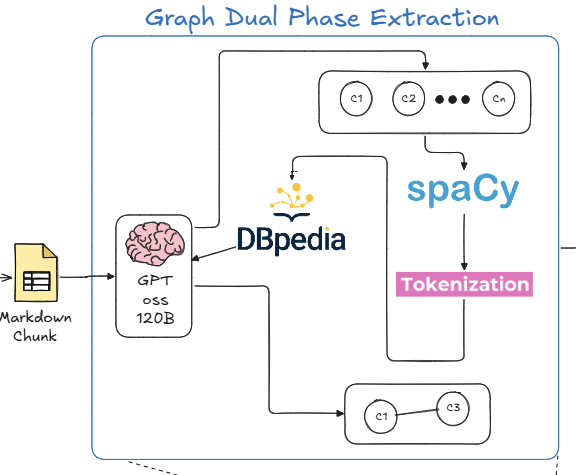
\includegraphics[width=0.65\textwidth]{Images/method/g_extract.png}
    \vspace{12pt}\caption{Dual Phase Extraction}\label{fig:g_ex}
\end{figure}
\subsubsection*{Phase 1: Top-Down Hierarchical Extraction (Skeleton Phase)}

The primary objective of the first phase is to establish the taxonomic structure of the knowledge domain without the cognitive burden of cross-referencing. The LLM's action space is strictly confined to identifying entities and their subsumption (parent-child) relationships.

We define the skeleton extraction function $\Phi_{\text{skeleton}}$ as:
\begin{equation}
    \Phi_{\text{skeleton}}: \mathcal{T} \rightarrow (V_{\text{tree}}, E_{\text{tree}})
\end{equation}
where $E_{\text{tree}} \subset V_{\text{tree}} \times V_{\text{tree}}$ contains strictly hierarchical edges (e.g., $ {PART\_OF}$).

To eliminate ontological drift, the LLM is forced to output data conforming to a rigid, predefined syntactic schema (e.g., strict JSON schema validation). The system parses this structural output to instantiate  {CommunityNode} and  {TopicNode} entities, ensuring that every atomic concept is firmly anchored to a macroscopic curriculum node.

Mathematically, this phase yields disjoint taxonomic trees. Because the LLM is only tasked with hierarchical assignment, the spatial complexity is bounded to $O(N)$ 
parent-child assignments. This drastic reduction in the problem space significantly mitigates the probability of generation errors. To complete the graph, phase 2 
is executed subsequently.

\subsubsection*{Phase 2: Lateral Relational Mapping (Relation Phase)}

With the hierarchical skeleton established as the logically structured frame, the second phase focuses on inferring the non-hierarchical, semantic linkages 
across different branches of the tree. Given the isolated, immutable entity set $V_{\text{tree}}$, the relational extraction function $\Phi_{\text{relation}}$ is 
defined as:
\begin{equation}
    \Phi_{\text{relation}}: (V_{\text{tree}}, \mathcal{T}) \rightarrow E_{\text{lateral}}
\end{equation}
where $E_{\text{lateral}}$ encompasses cross-cutting educational dependencies such as $ {PREREQUISITE\_OF}$ or $ {RELATED\_TO}$.

By presenting the LLM with a predefined, validated list of concepts ($V_{\text{tree}}$) and tasking it  {only} with edge generation, the problem space is reduced to a binary classification task over possible pairs. The final Educational Knowledge Graph is the formal union of these two sub-spaces: 
\begin{equation}
    G = (V_{\text{tree}}, E_{\text{tree}} \cup E_{\text{lateral}})
\end{equation}

To summarize, it is the operation of extracting potential candidate concepts as taxonomy trees and combine it to make a graph. This paradigm ensures high consistency 
in the generated graph. It bridges the gap between unstructured educational data and structured property graph by artificially 
constraining the LLM's action space, partlially preventing hallucinations. By partially, there is a big problem: Phase 2 relies mainly on Phase 1 for a structured and stable 
output, but what if Phase 1 itself is not a good frame skeleton? To better reconstruct and verify the frame, we use deterministic algorithm and techniques


\subsubsection{NLP-Based Concept Filtering and Verification}

The idea the Dual-Phase LLM Extraction (Section~\ref{subsub:dual}) is to reduces hallucination by constraining the model's action space of subsequent step using 
result from previous steps as an anchor and ground truth. However the raw output 
of Phase~1 remains inconsistence: semantically equivalent concepts may appear under distinct lexical forms, concepts extracted might not fit the full course content and
finally overly granular entities might be extracted just because it is mentioned once. In conclusion, using LLM to correct LLM has its limit. 
Inspired by BPE tokenization, a deterministic NLP pipeline is intergrated between Phase~1 
and Phase~2. This pipeline operates exclusively on the candidate node set $V_{\text{tree}}$ and produces a refined, verified set $V^{*} \subseteq V_{\text{tree}}$ 
that is subsequently passed to the Relation Phase. It is in fact a Entity Filterer proceeding through four sequential steps.

\paragraph*{Step 1 — Normalization and Tokenization.}

Each candidate concept label $v_i \in V_{\text{tree}}$ is first subjected to a standard text normalization procedure. This entails lowercasing, punctuation stripping, morphological lemmatization (reducing inflected word forms to their base lemma), and the removal of domain-agnostic stop words. The resulting form is then decomposed into a set of meaningful unigrams and bigrams, yielding a normalized token set $\mathcal{N}(v_i)$. Formally:
\begin{equation}
    \mathcal{N}(v_i) = \text{tokenize}\bigl(\text{lemmatize}(\text{lower}(v_i))\bigr) \setminus \mathcal{S}
\end{equation}
where $\mathcal{S}$ denotes the stop-word vocabulary. This normalization step establishes a canonical surface representation for every concept, ensuring that subsequent comparison operations are performed on semantically uniform token sets rather than raw, noisy strings.

\paragraph*{Step 2 — External Wiki Validation}

Following normalization, each candidate concept is submitted to the DBpedia Spotlight entity linking service. For a given concept $v_i$, the system issues a query against the DBpedia knowledge base to retrieve a set of $k$ candidate labels, denoted as $L_k$. 
To guarantee consistency and filter out unreliable terms, the system first identifies the most relevant label $l^*$ from the candidate set by maximizing the relevance score:
\begin{equation}
    l^* = \underset{l \in L_k}{\arg\max} \, \text{relevance}(l, v_i)
\end{equation}
Once the optimal label $l^*$ is identified, the concept is accepted and integrated into the knowledge graph only if this best match yields a positive relevance score:
\begin{equation}
    \text{relevance}(l^*, v_i) > 0
\end{equation}
If $\text{relevance}(l^*, v_i) = 0$, it indicates that even the most probable candidate of that entity definition yields no reliable definition on DBpedia. Concepts failing this 
criterion are usually either hallucinated constructs or excessively fine-grained pseudo-entities that lack grounding in established encyclopedic
 knowledge, and are subsequently pruned from $V_{\text{tree}}$. This external validation step introduces a strict layer of epistemic accountability, 
 anchoring the graph topology to verifiable, real-world semantics rather than model-generated approximations. 

 However, given the fact that todays researchers constantly discovering new paradigm and concepts that might have not been updated in Wiki, the system deliberately keeps 
 it as a Leaf Node with low weight. Though the node itself alone is not reliable, if its surrounding nodes are meaningful, its meaning can also be implicitly derived from 
 the graph structure, proposing a novel, robust architecture to new paradigm and innovation.
\paragraph*{Step 3 — Implicit Clustering}

Upon completion of filtering, the retained concepts undergo pairwise token similarity analysis. The Jaccard similarity between two concept representations is 
computed as:
\begin{equation}
    J(v_i, v_j) = \frac{|\mathcal{N}(v_i) \cap \mathcal{N}(v_j)|}{|\mathcal{N}(v_i) \cup \mathcal{N}(v_j)|}
\end{equation}

This measurement serves two complementary functions. First, concept pairs satisfying $J(v_i, v_j) \geq \tau_{\text{merge}}$ are treated as near-duplicates and 
consolidated into a single canonical node, thereby eliminating redundancy introduced by paraphrastic variation in the source text. Second, and more significantly, 
concepts that share a non-trivial common token subset — without necessarily crossing the merge threshold — are grouped into an  {implicit cluster}. The intersection 
$\mathcal{N}(v_i) \cap \mathcal{N}(v_j)$ is used to infer a shared parent topic label; for instance, the concepts ``Machine Learning Algorithms'' and ``Machine Learning Optimization'' 
both yield the shared token ``Machine Learning'', from which a  {TopicNode} bearing that label is derived. These implicitly discovered topic nodes are then cross-validated 
against the hierarchical skeleton produced by Phase~1 to either confirm existing  {TopicNode} entries or surface structural gaps in the original extraction.

\paragraph*{Step 4 — Node Caching.}

Once a concept node has successfully traversed Steps~1 through~3 — normalized, externally validated, and cluster-assigned — its canonical representation is persisted 
in a key-value cache, indexed by its normalized token set $\mathcal{N}(v_i)$. This cache serves three purposes. First, it ensures  {idempotency}: if the same concept surface form is encountered across multiple ingested documents, it resolves deterministically to the same canonical node without re-executing the NLP pipeline. Second, it supports  {incremental graph construction}: as new educational materials are added to the corpus over time, only genuinely novel concepts need to traverse the full verification pipeline, while previously verified nodes are retrieved directly from cache. Third, it provides the Relation Phase (Phase~2) with a stable, pre-validated entity vocabulary, eliminating the need for redundant lookups during edge generation. The final verified and deduplicated set $V^{*}$ is then passed forward as the immutable input to $\Phi_{\text{relation}}$.
\section{Teaching Assistance}
The knowledge graph $G$ serves as the static, structural foundation of the system. However, real-time interaction with a human 
learner demands a dynamic, adaptive reasoning engine capable of navigating $G$ to produce personalized educational responses. 
A single monolithic language model, no matter how capable, cannot reliably handle the diverse reasoning tasks involved in 
tutoring---from classifying student intent, to retrieving factual content with minimal cost and latency, to generating structured 
lectures, to evaluating learning outcomes. Each of these tasks requires a different workflow design.

To address this challenge, the proposed system decomposes the tutoring process into a multi-agent workflow, where each reasoning 
step is handled by a dedicated agent node with its own tailored prompt, tools, and output schema. The following subsections 
describe the core architectural decisions that make this decomposition both practical and effective: its applied harnessing 
as well as workflow design.

\subsection{Agent Harnessing}

Rather than relying on a single, prompt-heavy LLM to manage all tutoring logic, the Teaching Assistant is structured as a collection of specialized agent nodes 
coordinated through what we term an {Agent Harness}. This term was officially recognized worldwide this year, refering to all the infrastructure 
and pipeline revolves around the LLM. My proposed harnessing techniques govern how each node receives its instructions, what context it can access, 
and what format its output must follow. The design philosophy, from this point called the  {''Single Paradigm''}, is straightforward --- 
each agent node should have exactly one responsibility tied to one instruction set, one consistent context, and exactly one input/output structure/schema definition. 

\subsubsection*{Chat Summarization and Memory Management}

As a tutoring session progresses, raw chat history accumulates rapidly---exhausting the model's context window and degrading reasoning quality. The system addresses this with a sliding-window memorization mechanism: each turn is condensed into a structured triplet ( {query} $\rightarrow$  {thought} $\rightarrow$  {answer}), retaining only 8 entries at any time.

This history is exposed selectively: lightweight classification nodes (e.g., the intent router) receive only heading summaries ( {skim} mode), while nodes requiring deeper context---such as lecture generation or evaluation---receive the full summarized messages.

\subsubsection{Tool Abstraction Design}

Direct LLM access to the system's databases (Neo4j, Milvus, MongoDB, MinIO) risks malformed queries, unauthorized access, and destructive writes. A tool abstraction layer therefore sits between each agent and the underlying infrastructure: each tool exposes exactly one well-defined function, and agents have no direct access to raw query languages.

These tools are pre-configured with the student's session context before any agent invocation, making each call a simple, self-contained operation from the agent's perspective. This design simultaneously simplifies the agent's decision space and enforces strict data isolation across sessions.

\subsubsection{State---based Harnessing}

Even with many traditional context optimization techniques, agents still prone to context overhead when too many task instruction and tools metadata are injected, 
weaken their performance by miles and increase hallucination
The Dynamic Harness resolves this through state-dependent context injection: each workflow node receives its own dynamically populated prompt at runtime. 
Retrieval nodes get only retrieval-specific 
instructions; evaluation nodes receive evaluation criteria; synthesis nodes additionally receive upstream reasoning from prior nodes---yielding a minimal, 
purpose-built context window per node that collectively produces coherent multi-step reasoning.

Achieving this per-node dynamism requires intercepting agent execution at each workflow step---something standard frameworks (LangChain, CrewAI, AutoGen) do not 
natively support, as they fix agent configuration at initialization.
The solution proposed is the \textit{Adaptive Middleware}, which maintains an internal registry of workflow node names. When invoked at a node, it inspects the 
current node identifier, retrieves its registered harnessing protocol, and reconstructs the agent's configuration before execution.

\begin{figure}[H]
    \centering
    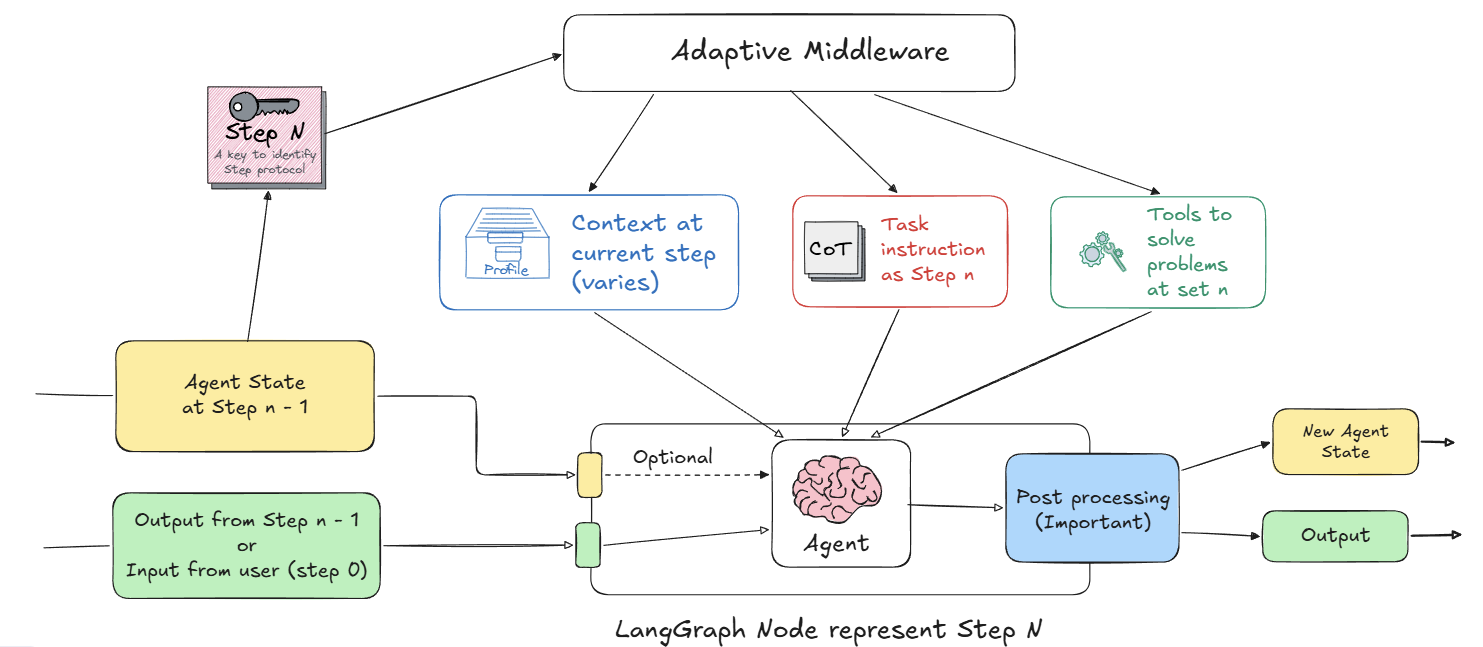
\includegraphics[width=1.0\textwidth]{Images/method/adaptive_middleware.png}
    \vspace{12pt}\caption{How agents's context and behaviour are constructed in a workflow node on a high level}\label{fig:agent2wf}
\end{figure}

This design offers 4 novel benefits:
\begin{enumerate}
 \item Single Paradigm is applied when a workflow node is registered with its own harnessing protocol, preventing the confusion that arises when a model must choose 
 among multiple possible reasoning paths, requirements, and methods.
 \item Because the middleware handles schema routing automatically, the prompt templates for each node can focus exclusively on the reasoning task at hand, without needing to include format-selection instructions.
 \item By constraining the output space to a predefined set, the system significantly reduces the probability of the model generating structurally invalid or semantically drifted responses. Each agent node operates within a tightly bounded action space---one task, one context, one schema---which collectively yields a more reliable and debuggable multi-step reasoning pipeline.
 \item With the registry techniques, agents are not hardcoded in nodes during initialization. This allows easy behaviour debug from the central registry, making agentic design more flexible and scalable.
\end{enumerate}

\subsubsection{Agentic Full Design}
Figure~\ref{fig:agent_harness} visualized a full harnessing of an agent, as well as its injection toward the workflow nodes to perform its task in a large 
LangGraph workflow, while table~\ref{tab:agent_tools} show us actionable protocols provided for agents in the form of Tools.

\begin{figure}[H]
    \centering
    \makebox[\textwidth][c]{
        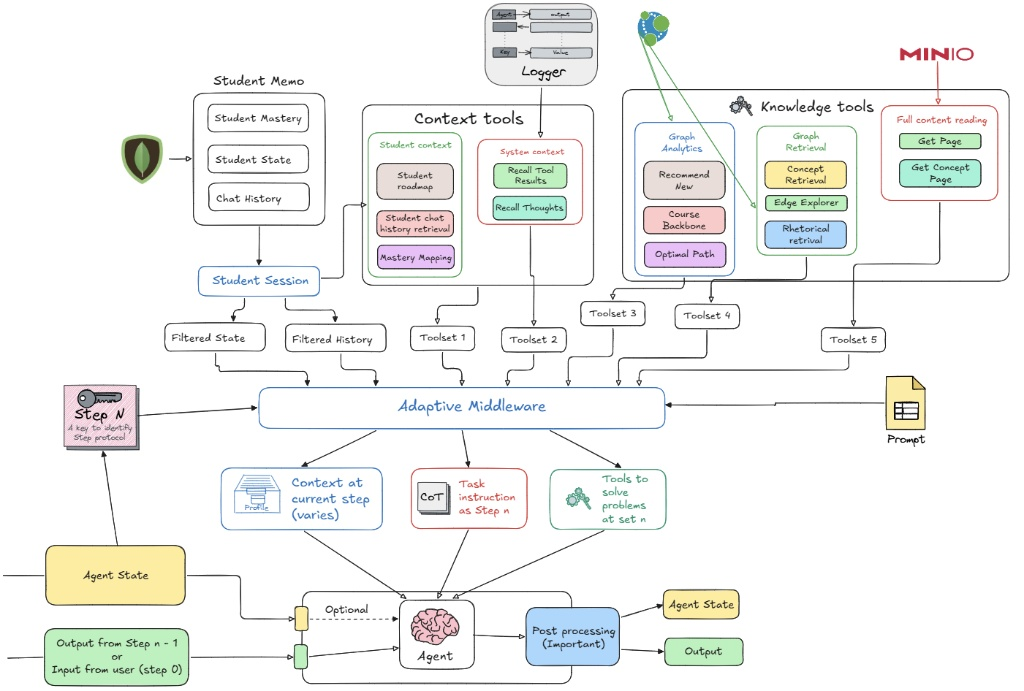
\includegraphics[width=1.1\textwidth]{Images/method/agent_design.jpg}
    }
    \vspace{12pt}\caption{Agent Harness architecture demonstrating the Adaptive Harnessing based on Middleware.}\label{fig:agent_harness}
\end{figure}

\begin{table}[H]
    \centering
    
    \renewcommand{\arraystretch}{1.3}
    \resizebox{\textwidth}{!}{
    \begin{tabular}{@{}llp{6.5cm}ll@{}}
        \toprule
        {Tool Name} & {Group} & {Description} & {Parameters} & {Database} \\
        \midrule
        \multicolumn{5}{@{}l}{{Context tools}} \\
        \midrule
        Student roadmap & Student context & Retrieve current student learning path and progress. &  {session\_id} & MongoDB \\
        Student chat history retrieval & Student context & Retrieve recent conversation history for context injection. &  {session\_id},  {limit} & MongoDB \\
        Mastery Mapping & Student context & Fetch student mastery scores for concepts. &  {session\_id} & MongoDB \\
        Recall Tool Results & System context & Retrieve recent tool execution results to prevent redundant calls. &  {limit},  {agent\_type} & Logger (In-memory) \\
        Recall Thoughts & System context & Retrieve recent agent reasoning traces for self-correction. &  {limit} & Logger (In-memory) \\
        \midrule
        \multicolumn{5}{@{}l}{{Knowledge tools}} \\
        \midrule
        Recommend New & Graph Analytics & Find top hub nodes ranked by out-degree for a starting point. &  {course\_filter},  {from\_node} & Neo4j \\
        Course Backbone & Graph Analytics & Extract course skeletal structure via top hub concepts and relations. &  {course\_name},  {max\_hubs} & Neo4j \\
        Optimal Path & Graph Analytics & Find the shortest weighted path between two concepts. &  {start\_node},  {end\_node} & Neo4j \\
        Concept Retrieval & Graph Retrieval & Resolve entity names to canonical IDs using graph or Wikidata. &  {query} & Neo4j \\
        Edge Explorer & Graph Retrieval & Explore multi-hop semantic relationships (excluding CONTENT edges). &  {node\_id} & Neo4j \\
        Rhetorical retrieval & Graph Retrieval & Retrieve educational content nodes by rhetorical role. &  {node\_id},  {role},  {limit} & Neo4j \\
        Get Page & Full content reading & Extract literal text from specific pages of a course document. &  {pages},  {destination} & MinIO \\
        Get Concept Page & Full content reading & Quickly locate page numbers referencing a specific concept. &  {concept} & Neo4j \\
        \bottomrule
    \end{tabular}
    }
    \caption{Summary of tools available to the Teaching Assistant agent.}
    \label{tab:agent_tools}
\end{table}

\newpage
\subsection{Agentic Workflow}

The Teaching Assistant's reasoning process is organized as a hierarchical state machine. At the top level, a router node classifies each incoming student query into 
one of five intent categories and dispatches it to the corresponding sub-workflow. Each sub-workflow is a directed graph of specialized nodes, where each node performs a single reasoning or data-retrieval step. Upon completion, every sub-workflow passes its results to a synthesis node that formats the final student-facing response and persists the session state. Figure~\ref{fig:smartedu} illustrates this top-level architecture.

\begin{figure}[H]
\centering
\begin{tikzpicture}[
  node/.style={rectangle, draw, rounded corners, minimum width=2.8cm,
               minimum height=0.7cm, font=\small, align=center},
  arr/.style={->, thick},
]

\node[node, fill=gray!20] (router) {TA\_Router\\{\tiny Intent Classification}};

\node[node, fill=green!15, below left=1.8cm and 0.4cm of router] (road) {WF\_Roadmap};
\node[node, fill=blue!15, left=0.6cm of road] (ret) {WF\_Retrieve};

\node[node, fill=orange!15, below right=1.8cm and 0.4cm of router] (teach) {WF\_Teach};
\node[node, fill=purple!10, right=0.6cm of teach] (prop) {Apply\_Proposal};

\node[node, fill=blue!8, below=1.5cm of ret] (retf) {TA\_Retrieve\_Finish};
\node[node, fill=green!8, below=1.5cm of road] (roadf) {TA\_Roadmap\_Finish};
\node[node, fill=red!10, below=4cm of router] (unk) {TA\_Unknown};
\node[node, fill=orange!8, below=1.5cm of teach] (teachf) {TA\_Teach\_Finish};

\node[node, fill=gray!30, below=7cm of router, minimum width=13.5cm] (end) {Session Context Saved\\(END)};

\draw[arr] (router) -- node[above left, font=\tiny, xshift=0.1cm] {retrieve} (ret.north);
\draw[arr] (router) -- node[left, font=\tiny, xshift=-0.1cm] {roadmap} (road.north);
\draw[arr] (router) -- node[right, font=\tiny, xshift=-0.1cm, yshift=-0.2cm] {unknown} (unk.north);
\draw[arr] (router) -- node[right, font=\tiny, xshift=0.1cm] {teaching} (teach.north);
\draw[arr] (router) -- node[above right, font=\tiny, xshift=-0.1cm] {confirm} (prop.north);

\draw[arr] (ret)  -- (retf);
\draw[arr] (road) -- (roadf);
\draw[arr] (teach) -- (teachf);

\draw[arr] (retf) -- (retf |- end.north);
\draw[arr] (roadf) -- (roadf |- end.north);
\draw[arr] (unk) -- (unk |- end.north);
\draw[arr] (teachf) -- (teachf |- end.north);
\draw[arr] (prop) -- (prop |- end.north);

\end{tikzpicture}
\vspace{10pt}
\caption{Top-level workflow routing based on user intents and context.}
\label{fig:smartedu}
\end{figure}

\subsubsection{Intent Router}

Every query must be dispatched to the correct sub-workflow before reasoning begins---misrouting wastes computation and produces structurally wrong responses. 
The router receives three inputs: (i) the student's current learning state, (ii) a  {skim}-mode chat summary, and (iii) the raw query---together disambiguating queries that appear identical but carry different intents across session contexts.

The prompting of the router goes for a straight forward {few-shot classification}: boundary-case examples for each routing choices. The output is a single constrained token 
from \{ {retrieve},  {roadmap},  {teaching},  {confirm},  {unknown}\} at temperature zero, with no tool invocation. This remove any time-cost reasoning chain, 
maximize speed and focus straight on real user input and well defined guildlines.

\subsubsection{Workflow: Roadmap}\label{subsub:wf_roadmap}

The Roadmap workflow addresses the planning problem:  {what should the student learn next, and in what order?} Unlike factual retrieval, this requires structural 
graph reasoning---the system must evaluate not only what exists in the knowledge base, but which concepts are most foundational, which the student has already 
mastered, and in what topological order they should be encountered. All structural analyses in this workflow consistently consider only semantic edges 
(prerequisite, hierarchical, associative) and explicitly exclude content-bearing edges, ensuring that centrality measures and path algorithms reflect 
presiquite dependency rather than rhetorical attachment.

\paragraph*{Out-Degree Centrality and Backbone Identification.}

The knowledge graph's density creates a navigation challenge---without a principled ranking, any learning path risks overwhelming the student or selecting concepts 
arbitrarily. The system addresses this with  {Out-Degree Centrality} as a structural heuristic. Heavily inspired by~\cite{DKG}, this is actually an algorithm to 
detect candidate central concept. Since the analytics is done on one type of edge, I propose a simplified version, ensured to be a built-in feature in Database. 
For a given node \(v\), the semantic out-degree \(C_{deg}(v)\) counts the number of outgoing semantic edges:

\begin{equation}
    C_{deg}(v) = \sum_{\substack{w \in V \\ (v,w) \in E_{\mathrm{sem}}}} 1
\end{equation}

where \(E_{\mathrm{sem}}\) excludes content-bearing edges. High-\(C_{deg}\) nodes serve as structural anchors and form the course backbone. 
This centrality measure is reused uniformly across all three sub-workflows: path planning (Roadmap), gap detection (Retrieve), and next-concept selection (Teach).

\paragraph*{Mastery State and the Knowledge Gap.}

The student's proficiency is represented as a  {mastery function} \(\mu : V \rightarrow [0, 1]\):

\begin{equation}
    \mu(v) =
    \begin{cases}
        s_v, & \text{if } v \in V_{\mathrm{explored}} \\
        0,   & \text{otherwise}
    \end{cases}
\end{equation}

where \(s_v \in [0,1]\) is the recorded Bloom's taxonomy mastery score for explored nodes, defaulting to zero otherwise. For any proposed backbone node \(b\), the set of unmastered prerequisites is:

\begin{equation}
    \Delta(b) = \{ u \in \mathcal{P}(b) \mid \mu(u) < \tau \}
\end{equation}

where \(\mathcal{P}(b)\) is the immediate prerequisite set of \(b\) and \(\tau\) is the mastery threshold. A non-empty \(\Delta(b)\) signals a knowledge gap that must be addressed before \(b\) is reachable.

\begin{figure}[H]
\centering
\begin{tikzpicture}[
  node/.style={rectangle, draw, rounded corners, minimum width=2.7cm,
               minimum height=0.8cm, font=\small, align=center},
  arr/.style={->, thick},
]
\node[node, fill=blue!15] (entry) {Entry Point:\\WF\_Roadmap};
\node[node, fill=cyan!10, right=1.5cm of entry] (explore) {Roadmap\_Explore\\{\tiny Pathway \& Hub Node Lookup}};
\node[node, fill=purple!10, right=1.5cm of explore] (eval) {Roadmap\_Evaluator\\{\tiny Feasibility vs Mastery Map}};
\node[node, fill=purple!10, below=1.2cm of eval] (advice) {TA\_Advice\\{\tiny Final Pedagogical Advice}};
\node[node, fill=gray!20, left=1.5cm of advice] (end) {Sub-graph END};

\draw[arr] (entry) -- (explore);
\draw[arr] (explore) -- (eval);
\draw[arr] (eval) -- (advice);
\draw[arr] (advice) -- (end);
\end{tikzpicture}
\vspace{10pt}
\caption{Roadmap sub-graph.}
\label{fig:roadmap_wf}
\end{figure}

Given the student's current position $v_{\mathrm{cur}}$, the system identifies the course backbone---its most foundationally connected concepts, ranked by $C_{deg}$---and computes the shortest prerequisite path to each backbone hub $b_i$ over the prerequisite sub-graph:
\begin{equation}
    \mathrm{Path}(v_{\mathrm{cur}},\, b_i) = [v_1, v_2, \ldots, v_k]
\end{equation}
These paths are merged and topologically sorted into a candidate list $\mathcal{L}$. To keep the result navigable, a sliding window retains only the top-$k$ nodes by $C_{deg}$ per segment $W_i \subset \mathcal{L}$:
\begin{equation}
    \mathrm{Selected}(W_i) = \operatorname{top\text{-}k}(W_i,\; C_{deg})
\end{equation}
yielding a condensed path where prerequisites always precede the concepts that depend on them:
\begin{equation}
    P_{\mathrm{roadmap}} = \mathrm{Selected}(W_1) \oplus \mathrm{Selected}(W_2) \oplus \cdots \oplus \mathrm{Selected}(W_m)
\end{equation}

Before the proposal reaches the student, it passes through a \textit{critic-actor} pass: a dedicated evaluator cross-references each backbone node against $\mu$, checking for unresolved gaps $\Delta(b) \neq \emptyset$, gatekeeper necessity, and cognitive load across the sequence. Its structured critique is then reconciled by an advisory agent into actionable guidance. Crucially, the resulting \textit{Learning Proposal} requires explicit student confirmation before modifying session state---unlike the auto-applied bridge proposals of the Retrieve workflow. Changing an entire learning trajectory is a high-stakes decision; the system is designed to inform and consent, not act unilaterally.

\subsubsection{Workflow: Retrieve}\label{subsub:wf_retrieve}

The Retrieve workflow answers factual questions by navigating the Educational Knowledge Graph. The workflow separates retrieval into two tiers---a fast, bounded lookup that satisfies most queries, and an optional deep structural analysis that activates only when a significant knowledge gap is detected.

\begin{figure}[H]
\centering
\begin{tikzpicture}[
  node/.style={rectangle, draw, rounded corners, minimum width=3.0cm,
               minimum height=0.8cm, font=\small, align=center},
  arr/.style={->, thick},
]
\node[node, fill=blue!15] (entry) {Entry Point:\\WF\_Retrieve};
\node[node, fill=cyan!10, below=1.2cm of entry] (core) {RAG\_Core\\{\tiny Global RAG \& KG Lookup}};
\node[node, fill=purple!10, below=1.2cm of core] (dec) {Deep\_Decision\\{\tiny Evaluate Gap Analysis}};
\node[node, fill=cyan!10, below left=1.2cm and 0.8cm of dec] (deep) {rag\_deep\\{\tiny Bridge Concept Retrieval}};
\node[node, fill=gray!20, below right=1.2cm and 0.8cm of dec] (end) {Sub-graph END};

\draw[arr] (entry) -- (core);
\draw[arr] (core) -- (dec);
\draw[arr] (dec) -- node[left, font=\tiny, xshift=-0.1cm] {\_deep\_route == 'deep'} (deep);
\draw[arr] (dec) -- node[right, font=\tiny, xshift=0.1cm] {\_deep\_route == 'skip'} (end);
\draw[arr] (deep) -- (end);
\end{tikzpicture}
\vspace{10pt}
\caption{Retrieval sub-graph. The flow routes dynamically to deep verification of prerequisite concepts if potential knowledge gaps are identified.}
\label{fig:retrieve_wf}
\end{figure}

The two-tier design reflects a deliberate efficiency-first principle: the majority of factual queries are definitional and can be resolved with a single graph traversal---resolving the concept to a canonical entity and fetching its rhetorical content (definition, formula, theorem, example). Forcing deep structural analysis on every query would inflate latency without benefit. A dedicated no-tool classifier therefore makes a binary routing decision after the initial lookup: simple queries exit directly to synthesis, while relational queries (\textit{how does X relate to Y}) activate the deep tier.

When deep analysis is triggered, the workflow shifts from content retrieval to \textit{structural gap bridging}: it traverses multi-hop semantic relationships to identify prerequisite nodes on the path between the student's current position and the queried concept, ranked by $C_{deg}$. A knowledge gap score $\gamma \in [0,1]$ quantifies the structural distance, and identified bridge concepts are packaged into a proposal that is applied automatically---reflecting the lower stakes of a targeted path adjustment compared to a full roadmap change.

\subsubsection{Workflow: Teach}\label{subsub:wf_teach}

The Teach workflow manages the continuous learning loop, delivering lectures, assessing mastery, and advancing the student's knowledge state through iterative interaction.

\begin{figure}[H]
\centering
\begin{tikzpicture}[
  node/.style={rectangle, draw, rounded corners, minimum width=3.0cm,
               minimum height=0.8cm, font=\small, align=center},
  arr/.style={->, thick},
]
\node[node, fill=blue!15] (entry) {Entry Point:\\WF\_Teach};
\node[node, fill=purple!10, below=1.0cm of entry] (und) {Teach\_Understand\\{\tiny Teaching Intent Classification}};
\node[node, fill=brown!10, below left=1.2cm and 1.8cm of und] (lkp) {Teach\_Lookup\\{\tiny Deterministic PDF Lookup}};
\node[node, fill=purple!10, below right=1.2cm and 1.8cm of und] (eval) {Teach\_Evaluate\\{\tiny Assess Learning Answers}};

\node[node, fill=cyan!10, below=1.2cm of lkp] (rag) {Teach\_RAG\\{\tiny RAG Fallback Query}};
\node[node, fill=orange!15, right=1.2cm of rag] (lec) {Teach\_Lecture\\{\tiny TA Lecture Generation}};
\node[node, fill=purple!10, below=1.2cm of eval] (nxt) {Next\_Topic\\{\tiny GraphDB Recommendation}};
\node[node, fill=gray!20, below=2.6cm of lec] (end) {Sub-graph END};

\draw[arr] (entry) -- (und);
\draw[arr] (und) -- node[left, font=\tiny, xshift=-0.1cm] {\_teach\_mode $\in$ ['continue', 'review']} (lkp);
\draw[arr] (und) -- node[right, font=\tiny, xshift=0.1cm] {\_teach\_mode == 'evaluate'} (eval);

\draw[arr] (lkp) -- node[left, font=\tiny] {source == NO\_CONTENT} (rag);
\draw[arr] (lkp) -- node[above, font=\tiny, yshift=0.1cm] {source == PDF} (lec);
\draw[arr] (rag) -- (lec);
\draw[arr] (eval) -- (nxt);

\draw[arr] (lec) -- (end);
\draw[arr] (nxt) |- (end);
\end{tikzpicture}
\vspace{10pt}
\caption{Teaching sub-graph flow: content lookup, RAG fallback, and adaptive topic progression.}
\label{fig:teach_wf}
\end{figure}

The central design philosophy is a \textit{Socratic loop}: deliver content, elicit a response, assess understanding, and either advance the student's position in the EKG or reinforce the current concept. A fine-grained entry classifier distinguishes three teaching modes---\textit{continue} (advance), \textit{review} (revisit), and \textit{evaluate} (assess)---ensuring the same surface query maps to the correct instructional behavior given the session state.

Content collection for lecture generation uses an iterative Reason-Act (ReAct) loop rather than a single retrieval call, allowing the agent to reason about what material is still needed and continue calling tools until the context $\mathcal{C}$ is sufficient (Figure~\ref{fig:react_teach}). Two tools drive this loop: \texttt{get\_concept} resolves the current node to a structured document reference (ID, MinIO path, page number), and \texttt{get\_pages} extracts the corresponding PDF pages; if no direct reference exists, the flow falls back to the Retrieve pipeline.

\begin{figure}[H]
\centering
\begin{tikzpicture}[
    node distance=1.4cm and 2.2cm,
    every node/.style={font=\small},
    startstop/.style={rounded rectangle, draw, fill=blue!8, minimum width=2cm, minimum height=0.7cm, align=center},
    action/.style={rectangle, draw, fill=green!8, minimum width=2.2cm, minimum height=0.7cm, align=center},
    decision/.style={diamond, draw, fill=orange!10, minimum width=1.2cm, minimum height=0.7cm, align=center, aspect=2.2},
    arr/.style={->, >=stealth, thick},
    darr/.style={->, >=stealth, thick, dashed}
]
    \node[startstop] (input) {Input Query};
    \node[action, right=of input] (context) {Context\\$C = [\text{input}]$};
    \node[decision, right=of context] (decide) {Sufficient?};
    \node[action, below=1.2cm of decide] (tool) {Tool Call:\\get material};
    \node[startstop, right=of decide] (output) {To Lecture\\Node};

    \draw[arr] (input) -- (context);
    \draw[arr] (context) -- (decide);
    \draw[arr] (decide) -- node[above] {\scriptsize Yes} (output);
    \draw[arr] (decide) -- node[right] {\scriptsize No} (tool);
    \draw[darr] (tool.west) -- ++(-1.8,0) node[midway, below, font=\scriptsize] {$C \leftarrow C \oplus \text{result}$} |- (context.south);
\end{tikzpicture}
    \vspace{12pt}\caption{ReAct loop in Teach Lookup.}\label{fig:react_teach}
\end{figure}

Lecture delivery is calibrated by the student's Bloom's taxonomy level: lower mastery receives definitions and grounded examples; higher mastery receives application problems and synthesis challenges. A closing challenge question is posed in \textit{continue} mode to close the teaching moment, while \textit{review} mode poses targeted recall questions over recently covered concepts. Assessment is deliberately tool-free---the agent judges mastery from conversational evidence alone, distinguishing genuine conceptual understanding from surface-level recall. The binary verdict then drives the session forward: a passing judgment triggers an auto-applied \textit{advance} proposal that moves the student's graph position to a high-centrality neighboring concept ranked by $C_{deg}$; a failing judgment returns a STAY action, preserving the current position for reinforcement.

\newpage
\chapter{System design and implementation}\label{chap:system}
This chapter presents the concrete design and implementation of the SmartEdu system, translating the methodology outlined in Chapter~\ref{chap:methodology} into a 
functioning software implementation. Such implementation are generalized in Figure~\ref{fig:pipeline}, an illustration of three principal flow paths through the system, functioning as a complete summarization of the 
operational pipeline.

\begin{figure}[H]
\centering
\resizebox{\textwidth}{!}{%
\begin{tikzpicture}[
  node distance=0.8cm and 1.0cm,
  box/.style={draw, rounded corners=3pt, minimum height=0.6cm, align=center, font=\tiny, fill=#1},
  db/.style={cylinder, draw, shape border rotate=90, minimum width=1.2cm, minimum height=0.7cm, font=\tiny, fill=#1, aspect=0.25},
  arr/.style={->, >=stealth, thick},
  lbl/.style={font=\tiny, midway, above},
  phase/.style={font=\footnotesize\bfseries, text=#1},
]
% === Path 1: Knowledge Ingestion ===
\node[phase=blue!70] at (0, 5.5) {Knowledge Ingestion};
\node[box=gray!15] (pdf) at (0, 4.8) {Raw PDF};
\node[box=blue!12] (parser) at (2.5, 4.8) {Parser};
\node[box=blue!12] (llm) at (5.0, 4.8) {LLM Extraction};
\node[box=blue!12] (builder) at (7.5, 4.8) {Graph Builder};
\node[db=purple!12] (neo_k) at (10.5, 5.3) {Neo4j};
\node[db=red!12] (milvus) at (10.5, 4.3) {Milvus};
\node[db=yellow!15] (minio) at (2.5, 3.8) {MinIO};
\draw[arr] (pdf) -- (parser);
\draw[arr] (parser) -- (llm);
\draw[arr] (llm) -- (builder);
\draw[arr] (builder) -- node[lbl]{entities} (neo_k);
\draw[arr] (builder) -- node[lbl, below]{embeddings} (milvus);
\draw[arr] (pdf) -- node[lbl, left]{archive} (minio);
% === Path 2: Student Lifecycle ===
\node[phase=green!60!black] at (0, 2.5) {Student Lifecycle};
\node[box=gray!15] (login) at (0, 1.8) {Login};
\node[db=green!12] (sqlite) at (2.5, 1.8) {SQLite};
\node[box=green!10] (session) at (5.0, 1.8) {Session Start};
\node[db=orange!12] (mongo) at (7.5, 1.8) {MongoDB};
\node[db=purple!12] (neo_s) at (10.5, 1.8) {Neo4j};
\draw[arr] (login) -- node[lbl]{credentials} (sqlite);
\draw[arr] (sqlite) -- node[lbl]{JWT} (session);
\draw[arr] (session) -- node[lbl]{state init} (mongo);
\draw[arr, dashed] (mongo) -- node[lbl]{mastery sync} (neo_s);
% === Path 3: Runtime ===
\node[phase=red!70] at (0, 0) {Runtime Interaction};
\node[box=gray!15] (query) at (0, -0.7) {Student Query};
\node[box=red!10] (ta) at (3.0, -0.7) {TA Workflow};
\node[db=orange!12] (mongo2) at (6.5, -0.7) {MongoDB};
\node[box=red!10] (tracer) at (6.5, -1.7) {Tracer};
\node[box=violet!10] (langfuse) at (9.5, -0.7) {Langfuse};
\draw[arr] (query) -- (ta);
\draw[arr] (ta) -- node[lbl]{memo + state} (mongo2);
\draw[arr] (ta) -- node[lbl, below]{traces} (tracer);
\draw[arr] (tracer) -- node[lbl]{flush} (langfuse);
% Cross-references
\draw[arr, dotted, gray] (neo_k) -- node[right, font=\tiny, text=gray]{entity id} (neo_s);
\draw[arr, dotted, gray] (milvus.south) -- ++(0,-1.2) -| node[below, font=\tiny, text=gray, near start]{vector search} (ta);
\end{tikzpicture}%
}
    \vspace{12pt}\caption{System general pipeline flow. Arrows show read - write operation direction}\label{fig:pipeline}
\end{figure}

As illustrated in Figure~\ref{fig:pipeline}, the system modules share data and state information across different pipelines utilizing common databases. 
This choice is necessitated by storage limits and hardware resource constraints. However, granting multiple modules access to the same storage engines introduces 
significant synchronization risks. To mitigate these risks, the architectural design enforces an universal constraint across the system:
While modules shares common infrastructures, 
  they perform internal logical operations in strict isolation. No logical module is allowed to directly invoke or interfere with the logic of another, 
  maintaining clean boundaries through dependency inversion. Modules cannot override other module results, or have effect in any way possible.

In the pursuit of implementing a robust system that satisfies these constraints, the subsequent sections present the optimal implementations, 
design paradigms, and structural layouts covering the following aspects:
\\\\{I. System Architecture and Design Patterns:} A high-level description of the system's architecture, components, their responsibilities and 
    interactions. It underlies design choices and principles that ensure modularity, scalability, and maintainability.
  \\\\{II. Core Module:} The foundational utility supporting all other modules, including LLM inference engine management, database clients, 
    centralized configuration handling, and shared data schemas.
\\\\{III. Database Design:} An overview of the polyglot persistence DB design, database cross reference and detailed explanation of the "One-Write" 
    policy solving the constraint.
\\\\{IV. Student Module:} The implementation of authentication, session management, and the Student Tracker façade, which abstracts away persistence details 
    while enforcing strict privacy.
\\\\{V. Knowledge Module:} The offline ingestion pipeline responsible for constructing the educational knowledge graph from raw course materials, covering extraction, 
transformation, and load operations.
\\\\{VI. Teaching Assistant (TA) Module:} Explain how LangGraph framework are used in the implementation of agentic workflow.
% ─────────────────────────────────────────────────────────────────────────────
\section{System Architecture}\label{sec:arch}
% ─────────────────────────────────────────────────────────────────────────────
\subsection{Overall Architecture and Module Responsibilities}

The SmartEdu backend is a monolithic FastAPI application composed of five functionally distinct, loosely coupled modules. 
This {Modular Monolith} design was deliberately architectured such that: consolidating modules into a 
single process eliminates network-induced latency between the components of the multi-step agentic workflow, while the strict dependency 
inversion between modules (discussed in Section~\ref{sec:nonfun}) ensures that each module can be extracted into an independent microservice 
with no changes to its internal business logic.

\begin{table}[H]
\centering
\caption{System Module Summary}\label{tab:modules}
\begin{tabular}{p{2.2cm} p{5cm} p{5cm}}
\hline
{Module} & {Primary Responsibility} & {Key Classes} \\
\hline
 {core}      & Shared infrastructure: LLM engine, all DB repository clients, configuration, shared schemas. &  {CoreLLMEngine},  {GraphDB},  {MilvusDB},  {MinioDB} \\
 {student}   & Authentication, session lifecycle, unified learning-state façade.   &  {Student\_Tracker},  {StudentSession},  {Memo} \\
 {knowledge} & Offline EKG construction pipeline from raw course materials.        &  {KnowledgeModule},  {CourseIngestionService} \\
 {TA}        & Real-time agentic workflow; generates pedagogically grounded responses. &  {TAModule},  {SmartEdu},  {AgentInjector} \\
 {tracing}   & Per-session observability; async trace buffering and Langfuse flush. &  {AgentTracer},  {TraceWriter} \\
\hline
\end{tabular}
\end{table}

The inter-module dependency graph is strictly acyclic:  {core} is the sole shared foundation depended on by all other modules;  {student},  {knowledge}, and  {TA} are peer modules that do not import one another;  {tracing} is consumed exclusively by  {TA}. 
This topology is illustrated in Figure~\ref{fig:sys_}.

\begin{figure}[H]
\centering
\begin{tikzpicture}[
  mod/.style={rectangle, draw, rounded corners, minimum width=2.6cm, minimum height=0.75cm, font=\small, align=center},
  db/.style={cylinder, draw, shape border rotate=90, minimum width=1.2cm, minimum height=0.6cm, font=\tiny, align=center},
  arr/.style={->, thick, gray},
  node distance=1.5cm and 2.1cm
]

\node[mod, fill=gray!20]              (core)     {\texttt{core}\\{\tiny Shared Infrastructure}};
\node[mod, fill=blue!12,  above=of core]  (student)  {\texttt{student}\\{\tiny Identity \& State}};
\node[mod, fill=green!12, above left=of core]       (knowledge){\texttt{knowledge}\\{\tiny KG Pipeline}};
\node[mod, fill=orange!12,above right=of core] (ta)       {\texttt{TA}\\{\tiny Agentic Workflow}};
\node[mod, fill=purple!10,below=of ta]         (tracing)  {\texttt{tracing}\\{\tiny Observability}};
\node[mod, fill=gray!20,below=of tracing]              (langfuse)     {\texttt{Langfuse}\\{\tiny Tracing cloud/endpoint}};

\node[db, fill=red!10, below left=of core] (neo)    {Neo4j\\(KG)};
\node[db, fill=yellow!10, left=of core] (mil)    {Milvus\\(Vector)};
\node[db, fill=blue!10, below=of core] (minio)  {MinIO\\(Filestore)};
\node[db, fill=green!10, below=of neo] (mongo)  {MongoDB\\(State)};
\node[db, fill=gray!10, below=of langfuse] (sql)    {MySQL\\(Credentials)};

\draw[arr] (student)   --node[midway, fill=white] {\tiny Access resources} (core);
\draw[arr] (knowledge) --node[midway, fill=white] {\tiny Access resources} (core);
\draw[arr] (ta)        --node[midway, fill=white] {\tiny Access resources} (core);
\draw[arr] (tracing)        --node[midway, fill=white] {\tiny Observe} (ta);
\draw[arr] (student)        --node[midway, fill=white] {\tiny Grant access} (ta);

\draw[arr] (core) --node[midway, fill=white] {\tiny Manage resources} (neo);
\draw[arr] (core) --node[midway, fill=white] {\tiny Manage resources} (mil);
\draw[arr] (core) --node[midway, fill=white] {\tiny Manage resources} (minio);
\draw[arr] (core) --node[midway, fill=white] {\tiny Manage resources} (mongo);
\draw[arr] (core) --node[midway, fill=white] {\tiny Manage resources} (sql);

\draw[arr] (tracing) --node[midway, fill=white] {\tiny push and configure} (langfuse);
\end{tikzpicture}
\vspace{12pt}
\caption{Modular Architecture Overview of SmartEdu}\label{fig:sys_}
\end{figure}

\subsection{Technical Setup: Docker Infrastructure}

The system's five database engines and their supporting services are deployed as Docker containers, orchestrated through a modular Docker Compose configuration. A root compose file includes per-engine definition files, each specifying one service and its dependencies. All containers communicate over a shared bridge network.

\begin{table}[H]
\centering
\caption{Docker Compose service summary.}
\label{tab:docker_services}
\renewcommand{\arraystretch}{1.2}
\begin{tabularx}{\textwidth}{|l|l|l|l|X|}
\hline
Service & Image & Memory & Ports & Role \\ \hline
neo4j-core & neo4j:2025-enterprise & 4 GB & 7474, 7687 & Knowledge and Student graph databases with APOC and GDS plugins \\ \hline
mongo-core & mongo:latest & 2 GB & 27018 & Student state, chat memo, and session context persistence \\ \hline
milvus-standalone & milvusdb/milvus:v2.4.0 & 2.5 GB & 19530 & Vector similarity search engine for concept embeddings \\ \hline
minio-core & minio/minio:latest & 1.5 GB & 9000, 9001 & S3-compatible object storage for PDF materials and text chunks \\ \hline
etcd & coreos/etcd:v3.5.5 & --- & --- & Metadata store required by Milvus for distributed coordination \\ \hline
attu & zilliz/attu:latest & 512 MB & 8000 & Web-based GUI for Milvus collection inspection and debugging \\ \hline
dbgate & dbgate/dbgate & --- & 3000 & Unified database administration interface for MongoDB \\ \hline
\end{tabularx}
\end{table}

The root compose file uses the ``include'' directive to import per-service YAML definitions, keeping each engine's configuration isolated and independently version-controlled. All services join a single shared bridge network, enabling inter-container communication by container name. Health checks are configured for critical services (Neo4j, MinIO, etcd) to ensure that dependent containers only start after their prerequisites are verified as operational.

\subsection{Design Paradigm}


\subsubsection{Singleton}\label{sub:singleton}


Common system design faces a central engineering challenges: expensive, long-lived resources — LLM model instances and database connection pools — are costly opration. 
Constructing these resources per-request would incur prohibitive latency and memory exhaustion. 
Optimization for a smooth system requires centralized resource management systems instead of reconstructing stateless models and connections over and over across code base.
\begin{figure}[H]
\centering
\begin{tikzpicture}[
  cls/.style={rectangle, draw, minimum width=2.8cm, minimum height=0.7cm, font=\small\ttfamily, align=center},
  own/.style={->, thick, dashed},
  node distance=1.4cm and 1.2 cm
]
\draw[thick, gray!60]
(-5,0.7) node[left, black] {\small \textbf{Application Layer}} -- (7,0.7);

\node[cls, fill=gray!15]  at (-3,-0.2)           (ls)  {lifespan()};
\node[cls, fill=yellow!15, right=of ls]  (st)  {app.state};

\draw[thick, gray!60]
(-5,-1.3) node[left, black] {\small \textbf{Resource Layer}} -- (7,-1.3);

\node[cls, fill=blue!10,   below left=of st]   (llm) {CoreLLMEngine};
\node[cls, fill=blue!10,   below=of st]      (gdb) {GraphDB};
\node[cls, fill=blue!10,   below right=of st](db) {Database};
\draw[thick, gray!60]
(-5,-3.1) node[left, black] {\small \textbf{Logical Layer}} -- (7,-3.1);

\node[cls, fill=green!10,  below=of llm]    (km)  {KnowledgeModule};
\node[cls, fill=orange!10, below=of gdb]     (ta)  {TAModule};
\node[cls, fill=purple!10, below=of db]     (str) {Student\_Tracker};

\draw[own] (ls) -- node[above,font=\tiny]{stores} (st);
\draw[own] (st) -- (llm); \draw[own] (st) -- (gdb); \draw[own] (st) -- (db);
\draw[->]  (llm) -- node[above,fill=white,font=\tiny]{inject} (km); \draw[->] (gdb) -- (km);
\draw[->]  (llm) -- node[above,fill=white,font=\tiny]{inject} (ta); \draw[->] (gdb) -- node[above,fill=white,font=\tiny]{inject} (ta); \draw[->] (str) -- node[above,font=\tiny]{inject} (ta);
\draw[->]  (db) -- node[above,fill=white,font=\tiny]{inject} (str); 
\end{tikzpicture}
\vspace{15pt}
\caption{Ownership graph in lifespan. Shared resources are injected into domain modules}\label{fig:lifespan}
\end{figure}

The solution lies in Figure~\ref{fig:lifespan}, illustrating the construction of application and initialization of subsequence resources and logic modules. 
The app lifecycle and its modules are managed through FastAPI's  {lifespan} context manager ( {core/api/life\_span.py}), which implements 
the  {Singleton} pattern at 
the application scope. During startup,  {lifespan} performs sequentially these actions:
\begin{enumerate}
  \item Configuration import: at the start, all configuration (database URIs, model names, API keys) is imported and centralized at the startup. This guaranteer
  that the entire application operates on a unified configuration for its entire lifetime. 
  \item Resources initialization: Resourse managers receive configs to 
  construct itself with completed methods and configs needed to init and manage resource instances like models, connection pools. 
  \item Life span allocates these managers on app.state, global and unique across the whole app. This behaviour guarantee: resources are easiliy accessed, and no matter 
  what logic below, the resources cannot be duplicated. All references will be guaranteed to be to the global instances, not copies. 
 \item On shutdown, it performs explicit disconnection and graceful resource realeases. Since all resources managers are Singleton directly managed by lifespan, the system
ensures no garbage instances or connection left when the app is down, leaving no burden to our hardware.
\end{enumerate}

 \subsubsection{Dependency Injection}
To further enhance FastAPI backend capability and Singleton Paradigm,the system proposes a dedicated  {Dependency Injection} (DI) layer in 
 {core/dependencies.py}. 
This file defines thin  {provider functions} — one per injectable resource — that each return the corresponding singleton from  {app.state}. 
Route handlers declare their dependencies as typed parameters annotated with  {Depends()}, and FastAPI's IoC container resolves and injects the correct 
costly instance at request time.

This indirection yields 4 engineering benefits:
\begin{itemize}
  \item {Decoupling of business logic:} Route handlers are pure functions of their typed inputs, completely unaware of how their dependencies are constructed.
  \item {Independence across all modules:} The injection allows no import needed. Therefore subsequence modules cannot import methods to create duplicates, further 
  strengthen Singleton Paradigm, and also avoid circular dependency caused by tangled import of shared components. It allows isolated refactorization or debug of functionality.
  \item {Flexible implementations:} Replacing even the most sentitive backbone infrastructure requires modifying only the 
  provider function, and changes are effective across all systems.
  \item {Testability:} The test suite overrides any provider via  {app.dependency\_overrides}, enabling full unit testing without live database or LLM connections.
\end{itemize}

\subsubsection{MVC-Aligned Module Structure}\label{sec:mvc}
The system is designed to support complex stateful workflows while remaining strictly modularity. Each domain module follows an MVC-aligned internal layout that enforces a clean separation of concerns:

\begin{itemize}
\item {Model (Schema):} Pydantic models defined in  {core/schema/} act
as the system-wide data contract. No module constructs ad-hoc dictionaries to 
communicate state; all inter-module data is typed and validated through shared classes —
for example,  {ConceptNode} and  {EduEdge} (graph ontology shared between 
Knowledge and TA modules),  {KG\_Instance} (Knowledge → Core contract), and 
 {LearningProposal} (TA → Student contract). This shared schema layer is what 
makes each module independently testable and replaceable.
  \item {Controller (API Router):} Each module exposes its functionality through a dedicated FastAPI router (e.g.,  {TA/api/route.py}). The router handles only HTTP-level concerns: parsing requests, invoking the service layer, and serializing responses. It contains no business logic.
  \item {Service (Domain Module):} Domain classes ( {TAModule},  {KnowledgeModule}) encapsulate all business logic. They receive infrastructure dependencies exclusively via constructor injection and communicate with the controller only through shared Pydantic schemas.
\end{itemize}

This strict layering has a crucial architectural consequence: because no module's business logic contains direct imports of another module's internal classes — only shared schemas from  {core} — each module can be extracted into an independent microservice by simply changing its entry point. The DI mechanism is replaced by an HTTP client call, and the Pydantic schemas serve as the API contract, with zero modification to domain logic. This makes the system  {scalable to microservices} by architectural design.



% ─────────────────────────────────────────────────────────────────────────────
\section{Core Module}\label{sec:core}
% ─────────────────────────────────────────────────────────────────────────────

The  {core} package is the dependency foundation of the entire system. It owns no domain business logic; instead, it supplies the primitive, reusable services 
and shared data contracts upon which all domain modules are built. As established in Section~\ref{sub:singleton}, all  {core} resources are constructed once 
during the lifespan phase and injected by reference.

\subsection{LLM Engine}

 {CoreLLMEngine} is the central gateway for all LLM interactions. It implements
the  {Multiton} pattern --- a generalization of Singleton where a fixed, named pool
of instances is managed. Internally it maintains a named registry of model connectors
keyed by a profile name. When an agent issues a model retrieval request, the
engine performs a cache lookup: if the profile is absent, it reads the corresponding
 {LLMProfile} from  {core/llm/config.py}, constructs a model connector
object, stores it in the registry, and returns it; subsequent calls for the same
profile return the cached object directly without reconstruction.

\subsubsection*{Lazy Instantiation and GPU Memory Lifecycle}

A critical property of this design is its  {zero-cost initialization}. Upon
construction, the engine's internal registry is empty --- no model weights are loaded
into GPU memory at application startup. A model connector is instantiated only on the
first retrieval request for a given profile, and only that specific model is loaded at
that moment. This ensures that GPU memory is occupied exclusively by models that have
been actively requested.

Memory retention after a request is governed by an idle retention timeout
configured per profile. This value is forwarded directly to the backend runtime,
which holds the model's weights in GPU memory for the specified duration after the last
inference call. Once the window expires, the runtime evicts the weights, freeing
resources for other workloads. The registered connector object persists in the cache;
the next invocation transparently triggers an automatic weight reload by the runtime.
Profiles without an explicit timeout inherit the runtime's global default retention policy.

The pairing of lazy instantiation with per-profile retention windows creates a tiered
memory strategy: high-frequency agents are kept warm for the full
duration of a tutoring session, moderate-frequency agents are
evicted after a shorter idle period, and lightweight classification workers
are evicted aggressively since their small size makes
cold-start reloads negligibly cheap.

\subsubsection*{Profile Configuration}

Each  {LLMProfile} dataclass encapsulates the full operational parameter set for
one agent role. Table~\ref{tab:llm_profiles} lists the six profiles defined in the
current deployment, along with the rationale for each configuration choice.

\begin{table}[H]
\centering
\caption{LLM Profile configurations and their engineering rationale.}
\label{tab:llm_profiles}
\renewcommand{\arraystretch}{1.3}
\resizebox{\textwidth}{!}{%
\begin{tabular}{@{}llcccp{5.5cm}@{}}
\toprule
\textbf{Profile} & \textbf{Model} & \textbf{Temp} & \textbf{Context (tok)} & \textbf{GPU Retention} & \textbf{Role and Rationale} \\
\midrule
\texttt{graph}     & gpt-oss:120b-cloud & 0.2  & 8\,192 & ---   & Knowledge graph extraction. Large context window accommodates full slide batches; low temperature enforces deterministic structured JSON output. \\
\texttt{ta}        & gpt-oss:120b-cloud & 0.67 & 4\,096 & 1 h   & Conversational tutor. Higher temperature yields more natural dialogue; kept hot in GPU memory for the full duration of a tutoring session. \\
\texttt{rag}       & qwen3:8b           & 0.0  & 2\,048 & 30 min & Retrieval reasoning agent. Temperature zero ensures deterministic tool-calling decisions; a fixed output token cap prevents runaway generation during structured output. \\
\texttt{evaluator} & qwen3:8b           & 0.3  & 2\,048 & ---   & Assessment nodes. Low temperature maintains a consistent scoring rubric across evaluations. \\
\texttt{generator} & gpt-oss:120b-cloud & 0.4  & 4\,096 & ---   & Lecture generation. Moderate temperature balances creative expression with factual grounding. \\
\texttt{worker}    & gemma3:1b          & 0.0  & 768    & 5 min & Lightweight intent classification. Smallest available model; minimal context and aggressive eviction keep resource cost negligible. \\
\bottomrule
\end{tabular}%
}
\end{table}

\subsection{Configuration Management}

All system configuration is expressed as Python  {@dataclass} objects in  {core/config.py}. Each subsystem has a dedicated configuration class —  {Neo} for the knowledge graph database,  {Mil\_conf} for the vector store,  ..... E
nvironment variables are read exactly once at module import time via  {python-dotenv}, which loads values from a centralized  {.env} file. The value are loaded once and 
binded into runtime via objects, guarantee consistent config setting and management. All dataclass fields default to sensible values if the corresponding variable is absent.
\begin{table}[H]
\centering
\caption{Configuration dataclasses.}
\label{tab:config_classes}
\renewcommand{\arraystretch}{1.3}
\resizebox{\textwidth}{!}{%
\begin{tabular}{@{}llp{4.5cm}p{5.5cm}@{}}
\toprule
\textbf{Class} & \textbf{Infrastructure} & \textbf{Key Parameters} & \textbf{Purpose} \\
\midrule
\multicolumn{4}{@{}l}{\textit{Infrastructure Connection Configs}} \\
\midrule
\texttt{Neo}         & Neo4j          & Connection URI, credentials, target database name    & Graph database connection. Instantiated twice: once for the knowledge graph (\texttt{test}), once for the student learning graph (\texttt{students}). \\
\texttt{Mil\_conf}   & Milvus         & Service URI, collection name, vector dimensionality (768), retry budget & Vector store connection for concept embedding storage and approximate nearest-neighbour similarity search. \\
\texttt{Emb\_conf}   & HuggingFace    & Model identifier, vector dimensionality (768), maximum token length & Embedding model parameters for scientific text vectorisation (default: SciBERT). \\
\texttt{Minio\_conf} & MinIO          & Service endpoint, access credentials, TLS flag       & Object storage connection for raw PDF course materials and extracted text chunks. \\
\texttt{Mongo\_conf} & MongoDB        & Host address, credentials, target database name      & Document store connection for student state, chat history, and session persistence. \\
\midrule
\multicolumn{4}{@{}l}{\textit{Module Logic Configs}} \\
\midrule
\texttt{Ingest\_param} & Knowledge pipeline & Source data path, pages per textbook batch (10), pages per slide batch (15) & Controls PDF chunking granularity during course ingestion; batch sizes tune the trade-off between LLM context utilisation and extraction precision. \\
\texttt{K\_conf}     & LLM Engine     & Extraction LLM profile name                         & Selects which model profile (see Table~\ref{tab:llm_profiles}) handles knowledge graph extraction tasks. \\
\texttt{TA\_conf}    & TA pipeline    & Agent name, system prompt, and output schema per agent & Declares the set of agents instantiated at startup; adding an entry is sufficient to register a new agent into the teaching workflow. \\
\texttt{Config\_Tracer} & Langfuse    & Enable flag, secret and public API keys, host URL    & Opt-in observability configuration; all fields default to empty strings, disabling telemetry silently when credentials are absent. \\
\midrule
\multicolumn{4}{@{}l}{\textit{Domain Model}} \\
\midrule
\texttt{Bloom}       & Mastery scoring & Six cognitive levels: Remember (1) through Create (6) & Defines the Bloom's Taxonomy ordinal scale used to represent and advance a student's conceptual mastery. \\
\bottomrule
\end{tabular}%
}
\end{table}



% ─────────────────────────────────────────────────────────────────────────────
\section{Database Design}\label{sec:database}
% ─────────────────────────────────────────────────────────────────────────────

The system employs a polyglot persistence strategy, distributing data across five specialised storage engines. 
Each engine is selected for its optimal alignment with the data modality it serves, allowing distributed micro manageable 
infrastructure.
\subsection{Polyglot Persistence Design}

\begin{table}[H]
\centering
\caption{Polyglot persistence strategy overview.}
\label{tab:polyglot}
\renewcommand{\arraystretch}{1.3}
\begin{tabularx}{\textwidth}{|p{1.8cm}|p{2.0cm}|X|X|}
\hline
\text{Engine} & \text{Data Type} & \text{System Role} & \text{Selection Rationale} \\ \hline
Neo4j & Graph data & Knowledge Graph (entities, edges, clusters) and Student Learning Graph (mastery, progress) & Optimised for multi-hop traversal and recursive prerequisite queries; native Cypher query language enables expressive graph pattern matching. \\ \hline
Milvus & Vector data & 768-dimensional SciBERT embeddings for semantic similarity search & Purpose-built for approximate nearest neighbour search using HNSW indexing; scales to millions of vectors with sub-millisecond query latency. \\ \hline
MongoDB & Document data & Student learning state, session context, chat memorisation, and tool result caching & Schema-flexible document store accommodating the variable structure of agent outputs; supports atomic field-level updates for concurrent session safety. \\ \hline
MinIO & Binary objects & Raw PDF course materials, extracted text chunks, and lecture assets & S3-compatible object storage decoupling binary files from the relational layer; erasure coding provides fault-tolerant parallel streaming. \\ \hline
SQLite & Relational data & Student authentication credentials and account metadata & Lightweight embedded database requiring zero configuration; enforces ACID properties for credential integrity without external service dependencies. \\ \hline
\end{tabularx}
\end{table}

\subsubsection{Neo4j: Knowledge and Learning Graphs}

The system maintains two logically separated graph databases on the same Neo4j instance, preventing cross-contamination between educational content and student progress data.

The Knowledge Database stores the Educational Knowledge Graph constructed by the Knowledge Module. Entity nodes carry the properties defined in Table~\ref{tab:node_props}, connected by the five edge types (PART OF, RELATED TO, PREREQUISITE OF, CONTENT, ELABORATES ON). The database enforces uniqueness constraints on both node identifiers and names, and maintains a full-text search index for efficient keyword-based retrieval. A dedicated index on the rhetorical role property enables the teaching workflow to perform role-filtered queries (e.g., retrieving only Definition-type nodes for explanatory responses).

The Student Database tracks individual learning progress. Each student is represented as a node connected to concept nodes via directed MASTERY edges. These edges carry a proficiency level (one through six, aligned with Bloom's Taxonomy) and a timestamp indicating the last assessment. The teaching workflow's Advance node writes to this database upon successful evaluation, creating new mastery edges or updating existing proficiency levels.

\begin{figure}[H]
\centering
\begin{tikzpicture}[
  node distance=0.8cm,
  entity/.style={draw, circle, minimum size=0.8cm, font=\tiny, fill=#1},
  edge_lbl/.style={font=\tiny, midway, above, sloped},
  title/.style={font=\small\bfseries, anchor=south},
]
% Knowledge DB
\node[title] at (2.5, 3.2) {Knowledge Database};
\draw[gray!40, rounded corners] (-0.5,-0.5) rectangle (5.5,3.0);
\node[entity=blue!15] (c1) at (0.5, 2) {Topic};
\node[entity=green!15] (c2) at (2.5, 2) {Concept};
\node[entity=green!15] (c3) at (4.5, 2) {Concept};
\node[entity=yellow!15] (r1) at (1.5, 0.5) {Rhet.};
\node[entity=yellow!15] (r2) at (3.5, 0.5) {Rhet.};
\draw[->, thick] (c1) -- node[edge_lbl]{PART OF} (c2);
\draw[->, thick] (c2) -- node[edge_lbl]{PREREQ} (c3);
\draw[->, thick] (c2) -- node[edge_lbl]{CONTENT} (r1);
\draw[->, thick] (c3) -- node[edge_lbl]{CONTENT} (r2);
% Student DB
\node[title] at (10, 3.2) {Student Database};
\draw[gray!40, rounded corners] (7.0,-0.5) rectangle (13.0,3.0);
\node[entity=red!15] (s1) at (8.0, 2) {Student};
\node[entity=green!15] (sc1) at (10.5, 2) {Concept};
\node[entity=green!15] (sc2) at (12.0, 0.5) {Concept};
\node[entity=green!15] (sc3) at (10.5, 0.5) {Concept};
\draw[->, thick] (s1) -- node[edge_lbl]{MASTERY L4} (sc1);
\draw[->, thick] (s1) -- node[edge_lbl, below]{MASTERY L2} (sc3);
\draw[->, thick, dashed] (sc1) -- node[edge_lbl]{PATH} (sc2);
\end{tikzpicture}
    \vspace{12pt}\caption{Neo4j dual-database schema. Knowledge and learning graphs separated.}\label{fig:neo4j_schema}
\end{figure}

\subsubsection{Milvus: Vector Embedding Index}

The Milvus vector database stores 768-dimensional SciBERT embeddings generated during the knowledge ingestion pipeline. Each record in the collection consists of three fields described in Table~\ref{tab:milvus_schema}.

\begin{table}[H]
\centering
\caption{Milvus collection schema.}
\label{tab:milvus_schema}
\renewcommand{\arraystretch}{1.2}
\begin{tabularx}{\textwidth}{|l|l|l|X|}
\hline
\text{Field} & \text{Data Type} & \text{Constraint} & \text{Description} \\ \hline
id & VARCHAR & Primary Key & Unique entity identifier, shared with Neo4j for cross-database reference \\ \hline
text & VARCHAR & --- & Concatenation of concept name and content, used as the embedding source text \\ \hline
embedding & FLOAT\_VECTOR (768) & Indexed & SciBERT-generated dense vector for semantic similarity search \\ \hline
\end{tabularx}
\end{table}

The collection employs a Hierarchical Navigable Small World (HNSW) index optimised for the L2 (Euclidean) distance metric. Table~\ref{tab:hnsw_config} details the index and search parameters.

\begin{table}[H]
\centering
\caption{HNSW index configuration.}
\label{tab:hnsw_config}
\renewcommand{\arraystretch}{1.2}
\begin{tabularx}{\textwidth}{|l|l|X|}
\hline
\text{Parameter} & \text{Value} & \text{Purpose} \\ \hline
M (bi-directional links) & 8 & Maximum number of neighbours per graph node during index construction \\ \hline
efConstruction & 64 & Search depth during index build; higher values improve recall at the cost of build time \\ \hline
ef (query-time) & 64 & Search depth during query; balances retrieval accuracy against latency \\ \hline
Metric Type & L2 (Euclidean) & Distance metric for approximate nearest-neighbour search \\ \hline
\end{tabularx}
\end{table}

\subsubsection{MongoDB: Student State and Session Context}

MongoDB serves as the primary persistence layer for all student-related runtime data. Each student is represented as a single document keyed by their unique identifier, containing three major nested structures:

Table~\ref{tab:mongo_fields} provides the detailed field-level schema of the student document.

\begin{table}[H]
\centering
\caption{MongoDB student document field schema.}
\label{tab:mongo_fields}
\renewcommand{\arraystretch}{1.2}
\begin{tabularx}{\textwidth}{|l|l|X|}
\hline
Field Path & Type & Description \\ \hline
\multicolumn{3}{|l|}{\textit{state (Learning State)}} \\ \hline
finished\_communities & Array & List of completed knowledge graph communities \\ \hline
current\_pos & Object / null & Currently active concept node in the learning path \\ \hline
active\_resource & String / null & Currently loaded material reference \\ \hline
mastery\_map & Object & Key-value map of concept name to Bloom's mastery level (0--6) \\ \hline
previous\_nodes & Array & Ordered history of recently visited concept nodes \\ \hline
upcoming\_nodes & Array & Queue of next recommended concepts from roadmap \\ \hline
summary & String & Compressed natural-language summary of learning progress \\ \hline
pending\_proposal & Object / null & Unconfirmed learning path update awaiting student approval \\ \hline
\multicolumn{3}{|l|}{\textit{memo (Chat History) --- nested by session\_id}} \\ \hline
role & String & Speaker identifier: ``student'' or ``TA'' \\ \hline
heading & String & Topic heading for memo display \\ \hline
message & String & Full message content \\ \hline
timestamp & DateTime & Server-side UTC timestamp \\ \hline
\multicolumn{3}{|l|}{\textit{session\_context --- nested by session\_id and chat\_id}} \\ \hline
tool\_results & Array & Cached tool execution outputs for within-request recall \\ \hline
thoughts & Array & Agent reasoning traces for debugging and observability \\ \hline
\end{tabularx}
\end{table}

All write operations use atomic field-level updates (MongoDB \$set and \$push operators) rather than full document replacement. This ensures that concurrent sessions belonging to the same student can safely update disjoint fields (e.g., one session updating the mastery map while another appends to the chat memo) without overwriting each other's changes.

MinIO provides S3-compatible object storage for all binary educational assets. All objects reside in a single bucket named ``courses''. The storage hierarchy follows a deterministic three-level path convention detailed in Table~\ref{tab:minio_tree}, enabling the teaching workflow to reconstruct any object path programmatically from the concept's source reference property.

\begin{table}[H]
\centering
\caption{MinIO bucket directory structure.}
\label{tab:minio_tree}
\renewcommand{\arraystretch}{1.2}
\begin{tabularx}{\textwidth}{|l|l|X|}
\hline
\text{Path} &\text{ Content Type} & \text{Description} \\ \hline
\texttt{courses/} & Bucket root & Single top-level bucket containing all course data \\ \hline
\texttt{\{course\}/\{material\}/\{material\}.pdf} & application/pdf & Original raw PDF archived at ingestion time \\ \hline
\texttt{\{course\}/\{material\}/chunks/\{chunk\_id\}.txt} & text/plain & Extracted text chunk stored individually for granular retrieval \\ \hline
\end{tabularx}
\end{table}

The deterministic naming convention ensures that any component in the system can reconstruct an object path from two known values: the course name and the material name. The TA workflow exploits this property to serve PDF page references directly to the student frontend without querying a separate metadata index.

\subsubsection{SQLite: Authentication Store}

Student authentication is managed through a lightweight embedded SQLite database. Table~\ref{tab:sqlite_schema} describes the schema of the single ``students'' table.

\begin{table}[H]
\centering
\caption{SQLite students table schema.}
\label{tab:sqlite_schema}
\renewcommand{\arraystretch}{1.2}
\begin{tabularx}{\textwidth}{|l|l|l|X|}
\hline
\textbf{Column} &\textbf{Type}  & \textbf{Constraint} & \textbf{Description} \\ \hline
id & TEXT & PRIMARY KEY & Unique student identifier \\ \hline
username & TEXT & UNIQUE & Login credential, enforced unique \\ \hline
name & TEXT & --- & Student display name \\ \hline
email & TEXT & --- & Contact email address \\ \hline
password & TEXT & --- & SHA-256 hashed password \\ \hline
created\_at & TIMESTAMP & DEFAULT NOW & Account creation timestamp \\ \hline
\end{tabularx}
\end{table}

The deliberate choice of an embedded database eliminates external service dependencies for authentication while providing ACID guarantees for credential operations. Password hashing uses SHA-256 at the application layer before storage.

\subsection{Cross-Database Reference and Consistency}
Multiple system modules access to multiple database, and a lot of data of different source are aggregated and updated during run time.
To stabilize this structure, two architectural paradigms govern how the five storage engines coexist without data duplication or race conditions.

\subsubsection*{Unique Key Cross-Database Reference}

Entity identifiers serve as the primary cross-reference between Neo4j and Milvus: the same string identifier stored as a node 
property in Neo4j functions as the primary key in the Milvus collection, enabling the RAG agent to seamlessly translate between 
graph traversal results and vector similarity searches. When an agent performs a semantic search in Milvus, the returned identifiers are directly usable as lookup keys in Neo4j Cypher queries, eliminating the need for an intermediate translation layer.

Student identifiers bridge SQLite (authentication), MongoDB (learning state), and the Neo4j Student Database (mastery graph). 
A single login event propagates the authenticated identity consistently across all three stores: SQLite validates the credential 
and returns the student identifier, which MongoDB uses as its document primary key, and which Neo4j uses as the Student node 
property. This shared key ensures that mastery updates written by the TA workflow in Neo4j are immediately visible when the 
Student Tracker reads the learning state from MongoDB, without any synchronisation protocol beyond the identifier itself.

\subsubsection*{One-Write Policy}

With consistent cross-database reference, modules can easily access many database, a dangerous convenience that may hinge race condion risk. 
To solve this, "One-Write Policy" is proposed: 
each database collection or table is assigned exactly one write-owning module, with strictly governed method. All other modules 
are restricted to read-only access. Table~\ref{tab:write_policy} enumerates the write ownership assignments.

\begin{table}[H]
\centering
\caption{Write ownership per database.}
\label{tab:write_policy}
\renewcommand{\arraystretch}{1.2}
\begin{tabularx}{\textwidth}{|l|l|l|X|}
\hline
\textbf{Database} & \textbf{Collection} & \textbf{Writer} & \textbf{Consumers} \\ \hline
Neo4j (Knowledge) & Entity nodes, edges & Knowledge Module & TA Module \\ \hline
Neo4j (Student) & Student, MASTERY edges & TA Module & Student Module \\ \hline
Milvus & Concept embeddings & Knowledge Module & TA Module \\ \hline
MongoDB & students collection & Student Module & TA Module \\ \hline
MongoDB & learning\_logs collection & Student Module & TA Module \\ \hline
MinIO & courses bucket & Knowledge Module & TA Module \\ \hline
SQLite & students table & Student Module & --- \\ \hline
\end{tabularx}
\end{table}

This strict ownership eliminates the possibility of two modules concurrently writing to the same field. Combined with MongoDB's 
atomic field-level update operators, the policy ensures that even within a single write-owning module, concurrent sessions 
update disjoint document paths without overwriting each other's changes.


% ─────────────────────────────────────────────────────────────────────────────
\section{Student Module}
% ─────────────────────────────────────────────────────────────────────────────

\subsection{Authentication: OAuth2 + JWT}

The student module implements a standard OAuth2 password flow using  {PyJWT} for JWT minting. The  {/student/login} endpoint 
validates credentials against SHA-256 hashed passwords in SQLite and returns a short-lived JWT ( {sub} =  {student\_id}). All 
subsequent requests attach this token as a Bearer credential;  {get\_current\_student()} (a FastAPI dependency) decodes and 
validates it on each call.

\subsection{Session Lifecycle and the Identity Firewall}\label{sec:firewall}

The idea of this module is to initiate access to sensitive components and resources and enable logic modules only after login, via a controlled restricted manner. 
Moreover, it must guarantee an abstracted, hidden access that cannot be fully comprehend from application layer, but can only invoke via monitored request protocols.

The discussed paradigms goes into practice by a authentication and permission granted through a session lifecycle design described in Figure~\ref{fig:student_login}. The 
proccess goes by:
\begin{enumerate}
  \item After login, the student calls  {POST /student/session/start} with their JWT. The server generates a random UUID ( {session\_id}) and registers it in  {Student\_Tracker}.
  \item All subsequent TA interactions supply only  {session\_id}. The TA Module never receives  {student\_id}.
  \item Inside  {Student\_Tracker.\_resolve()}, the private mapping  {session\_id → student\_id} translates transparently before any database call.
\end{enumerate}


\begin{figure}[H]
\centering
\resizebox{\textwidth}{!}{%
\begin{tikzpicture}[
  every node/.style={font=\small},
  box/.style={draw, rounded corners=4pt, minimum width=2.8cm, minimum height=0.75cm,
              align=center, fill=#1},
  arr/.style={->, >=stealth, semithick},
  lbl/.style={font=\scriptsize, align=center}, 
]
%% ── Phase 1: Session Initialisation ────────────────────────────────────
\node[box=blue!10]    (C1)  at (0,   2.5) {Client};
\node[box=green!12]   (SS)  at (5.5, 2.5) {Student Module\\[2pt]{\tiny /session/start}};
\node[box=violet!10]  (ST1) at (11.0, 2.5) {Student Tracker\\[2pt]{\tiny session registry}};

\draw[arr] (C1) -- node[above, lbl]{JWT} (SS);
\draw[arr] (SS) -- node[above, lbl]{register\\[1pt]$(s_\mathrm{id},\, u_\mathrm{id})$} (ST1);

\draw[arr] (SS.south) -- ++(0,-0.42) -- ++(-5.5, 0) -- (C1.south);
\node[lbl, below] at (2.75, 2.08) {return $s_\mathrm{id}$ (UUID)};

%% ── Phase 2: TA Interaction ─────────────────────────────────────────────
\node[box=blue!10]    (C2)  at (0,    0)  {Client};
\node[box=orange!10]  (TA)  at (5.5,  0)  {TA Module};
\node[box=violet!10]  (ST2) at (11.0,  0)  {Student Session\\[2pt]{\tiny resolve $(s_\mathrm{id}) \to u_\mathrm{id}$}};
\node[box=gray!15]    (DB)  at (15.0, 0)  {Databases};

\draw[arr] (C2)  -- node[above, lbl]{requests with\\[1pt]$s_\mathrm{id}$ only} (TA);
\draw[arr] (TA)  -- node[above, lbl]{invoke predefined methods\\[1pt]via $s_\mathrm{id}$} (ST2);
\draw[arr] (ST2) -- node[above, lbl]{$u_\mathrm{id}$} (DB);
\draw[arr] (ST1)  -- node[right, lbl]{allocate new\\[1pt](or cached)} (ST2);

%% ── Identity Firewall ───────────────────────────────────────────────────
\draw[dashed, thick, red!60] (8.25, -2.85) -- (8.25, 3.35);


%% ── Phase labels ────────────────────────────────────────────────────────
\node[font=\scriptsize\itshape, text=gray!75] at (5.5,  3.4)
    {Phase 1 --- Session Initialisation};
\node[font=\scriptsize\itshape, text=gray!75] at (5.5, -0.65)
    {Phase 2 --- TA Interaction};

%% ── Annotation ──────────────────────────────────────────────────────────
\node[draw, dashed, rounded corners=3pt, font=\scriptsize, text=gray!80,
      align=center, inner sep=4pt, fill=yellow!5] at (13.0, -0.88)
    {$u_\mathrm{id}$ never\\[1pt]exposed to TA};
\end{tikzpicture}%
}
    \vspace{12pt}\caption{Login protocol with Identity Firewall (represented by the red line).}\label{fig:student_login}
\end{figure}

This pattern is analogous to a hotel key-card system: the key (session\_id) grants access to resources, but revealing it does not expose the guest's credentials 
(student\_id). Most importantly, all modules, tools can only gain abstracted access to student metadata can only be done once login. This prevent dangerous activity 
from AI or outside parties to sensible databases and resources.

As such, {Student Tracker} acts as a Singleton Manager that provide, cache and clean resources of unused Session. In the current implementation, 
it manages two distinct layers of state:

\begin{enumerate}
    \item {Session-Specific State ( {StudentSession})}: Keyed by  {session\_id}, this layer isolates chat history and session-specific context (like recent PDF pages). This prevents "Identity Race Conditions" where multiple browser tabs contaminate each other's chat logs.
    \item {Shared Learning State}: Keyed by  {student\_id}, this layer caches the student's learning progress (current position, mastery map, etc.) and is shared across all active sessions of the same student.
\end{enumerate}

To ensure data integrity during concurrent updates, the tracker utilizes {Atomic Field Updates} in MongoDB. 
Instead of overwriting the entire state object, the system updates specific fields (e.g., updating only the  {current\_pos} or appending to  {finished\_communities}). 
This design effectively mitigates "Data Race Conditions" where one session might accidentally revert progress made in another concurrent session.

% ─────────────────────────────────────────────────────────────────────────────
\section{Knowledge Module}\label{sec:knowledge_module}
% ─────────────────────────────────────────────────────────────────────────────

The Knowledge Module operates as an offline administrative pipeline responsible for transforming raw educational documents into the structured Educational Knowledge Graph consumed by the Teaching Assistant at runtime. This module is accessible exclusively through a dedicated REST endpoint, invoked by administrators upon uploading new course materials.

\subsection{Technical Setup}

Table~\ref{tab:km_libs} summarises the principal libraries employed by the Knowledge Module. All dependencies are resolved through the \textit{uv} package manager, ensuring deterministic, lockfile-driven builds across development and deployment environments.

\begin{table}[H]
\centering
\caption{Knowledge Module core libraries.}
\label{tab:km_libs}
\renewcommand{\arraystretch}{1.3}
\begin{tabularx}{\textwidth}{|l|X|}
\hline
\textbf{Library} & \textbf{Role in Pipeline} \\ \hline
Docling & PDF parser that converts each page into structured text blocks with provenance metadata such as page number and bounding region. \\ \hline
spaCy & Natural language processing library providing lemmatisation, synonym resolution, and stopword filtering for the post-extraction deduplication stage. \\ \hline
Pydantic & Schema validation framework that enforces strict structural contracts on every LLM extraction output, rejecting malformed responses before graph insertion. \\ \hline
SciBERT & Domain-specific sentence transformer (768 dimensions) trained on scientific corpora, generating embeddings that capture academic semantic similarity. \\ \hline
\end{tabularx}
\end{table}

\subsection{Ingestion Workflow}

The ingestion pipeline supports two distinct material types---lecture slides and textbooks---each following a tailored processing path. Both paths share a common entry stage (document parsing and window segmentation as described in Section~\ref{subsub:sliding}), but diverge at the knowledge extraction stage due to the fundamentally different structural roles these materials serve in the educational knowledge base.

To maximize throughput and minimize hardware idle time, both pipelines are engineered as fully asynchronous systems. This architectural choice prevents blocking operations during heavy I/O tasks or Large Language Model (LLM) inference, effectively turning a sequential bottleneck into a continuous stream of data processing.

\begin{figure}[H]
\centering
\resizebox{0.95\textwidth}{!}{%
\begin{tikzpicture}[
    >=stealth, font=\sffamily,
    % Styles
    threadBox/.style={draw, thick, rounded corners=8pt, inner sep=15pt},
    actionNode/.style={draw, thick, fill=white, rounded corners=4pt, minimum width=2.8cm, minimum height=0.8cm, align=center},
    queueNode/.style={draw, thick, rounded corners=10pt, minimum width=3.5cm, minimum height=1cm, align=center},
    dbNode/.style={draw, thick, fill=gray!15, cylinder, shape border rotate=90, aspect=0.25, minimum width=1.4cm, minimum height=1.2cm, align=center}
]

% ================= DATABASES (Bờ ngoài cùng) =================
\node[dbNode] (minio) at (0, 4) {\textbf{MinIO}};
\node[dbNode] (neo) at (5, 0.0) {\textbf{Neo4j}};

% ================= CỘT 1: MAIN THREAD (Non-blocking) =================
\node[actionNode, draw=blue!80] (pdf) at (0, 6.5) {\textbf{pdf extractor}\\};
\node[actionNode, dashed, draw=gray, text=gray] (other) at (0, 1.5) {\textit{Main Thread Free}\\\textit{(Repeat PDF extraction...)}};

% ================= CỘT 2: MIDDLEWARE QUEUES (Buffer) =================
\node[queueNode, fill=purple!10, draw=purple!60] (q1) at (5, 6.5) {\texttt{extract\_queue}\\(Chunk Buffer)};
\node[queueNode, fill=green!10, draw=green!60] (q2) at (5, 4) {\texttt{build\_queue}\\(Graph Buffer)};

% ================= CỘT 3: ASYNC WORKER POOL =================
% 1. Parallel LLM Workers (Vẽ 3 hộp đè lên nhau tạo hiệu ứng Parallel)
\node[actionNode, fill=orange!10, draw=orange!80] (w3) at (10.6, 6.9) {\textbf{LLM Worker 2}};
\node[actionNode, fill=orange!10, draw=orange!80] (w2) at (10.8, 6.7) {\textbf{LLM Worker 1}};
\node[actionNode, fill=orange!10, draw=orange!80] (w1) at (11.0, 6.5) {\textbf{LLM Worker 0}};

% 2. Sequential Graph Constructor
\node[actionNode, fill=teal!10, draw=teal!80] (gc) at (5, 2.25) {\textbf{Graph Constructor}\\(Sequential)};


% ================= TIMELINE (Trục dọc) =================
\draw[->, thick, gray] (13, 7.5) -- (13, 0);
\node[right, font=\small] at (13, 6.5) {Time $t_0$};
\node[right, font=\small] at (13, 4.75) {Time $t_1$};
\node[right, font=\small] at (13, 3) {...............};
\node[right, font=\small] at (13, 1) {Time $t_n$};

% ================= ARROWS & ROUTING =================
% Main Thread activities
\draw[->, thick, blue!80] (pdf.south) -- (minio.north) node[midway, above, font=\scriptsize] {upload\_raw};
\draw[->, thick, blue!80] (pdf.east) -- (q1.west) node[midway, above, font=\scriptsize] {put(chunk)};
\draw[->, thick, dashed, gray] (minio.south) -- (other.north) node[midway, right, font=\scriptsize, align=left] {Keep running, No waiting};

% Queue 1 to Workers
\draw[->, thick, orange!80] (q1.east) -- (w1.west) node[midway, above, font=\scriptsize] {get()};

% Workers to Queue 2 (Đường chéo vắt ngược lại Buffer)
\draw[->, thick, orange!80] (w1.south) -- (q2.north east) node[midway, above right, font=\scriptsize, xshift=0.3cm] {put(sub-graph)};

% Queue 2 to Graph Constructor
\draw[->, thick, teal!80] (q2.south) -- (gc.north) node[midway, above, font=\scriptsize] {get()};

% Graph Constructor to Neo4j
\draw[->, thick, teal!80] (gc.south) -- (neo.north) node[midway, above, font=\scriptsize] {update()};

\end{tikzpicture}%
}
\vspace{15pt}\caption{Asynchronous Ingestion Pipeline integrating Queues, Parallel Workers, and Storage}
\label{fig:ingestion}
\end{figure}

Lecture slides follow the primary extraction path. Because slide extraction involves complex, interdependent LLM operations and strict database insertion rules, it is architected as a Three-Station Producer-Consumer pipeline interconnected by bounded asynchronous queues. This design guarantees that data extraction happens continuously without being bottlenecked by slower downstream database operations.

\begin{itemize}
    \item \textbf{Station 1 (Producer):} The operation on the main threads continuously parses the PDF document, chunking pages and immediately uploading the raw segments 
    to MinIO. As soon as a chunk is ready, it is pushed into the Extraction Queue, then it leaves all the work to the background consumer and move the next document.
    \item \textbf{Station 2 (LLM Workers):} A pool of concurrent worker coroutines consumes items from the Extraction Queue. These workers operate independently, 
    forwarding chunks to the LLM for the Dual-Phase Extraction (concept mapping and relation discovery). The asynchorous task are yielded to wait for the LLM 
    result from cloud, costing little memory but effectively reduces inference waiting times. Once the LLM yields the structural representation, the result is 
    forwarded to the Build Queue.
    \item \textbf{Station 3 (Graph Builder):} A single sequential getting extracted nodes, edges result from the Build Queue. It constructs the Knowledge Graph 
    and ensures safe, transaction-free graph updates to Neo4j. Keeping this station single-threaded intentionally prevents race conditions and topological conflicts 
    during the graph assembly phase, while the heavier workload (LLM inference) remains aggressively parallelized upstream.
\end{itemize}

Backpressure mechanisms are naturally enforced by setting maximum capacity limits on the interconnecting queues, ensuring that memory usage remains stable even if the 
PDF parsing station outpaces the LLM workers. Experiments shows that results are 30\% faster with this approach.


\subsection{Graph Schema at Database Level}

The Knowledge Graph stored in Neo4j follows the formal Property Graph definition established in Section~\ref{sub:g_def}. Each entity node carries a set of standardised properties that support both structural navigation and semantic retrieval:

\begin{table}[H]
\centering

\renewcommand{\arraystretch}{1.2}
\begin{tabularx}{\textwidth}{|l|X|}
\hline
Property & Description \\ \hline
Name & Canonical concept label, enforced unique across the database \\ \hline
Identifier & Machine-generated unique key for programmatic reference \\ \hline
Content & Full textual description or definition of the concept \\ \hline
Node Type & Ontological category: Community, Topic, Concept, or Rhetorical \\ \hline
Rhetorical Role & Instructional function (Definition, Theorem, Application), assigned only to Rhetorical-type nodes \\ \hline
Cluster & Community identifier assigned during graph construction \\ \hline
Source Reference & Serialised pointer to the original material location in object storage \\ \hline
\end{tabularx}
\vspace{12pt}\caption{Entity node properties in Neo4j.}
\label{tab:node_props}
\end{table}

Five directed edge types connect these entities: \textit{PART OF} (hierarchical containment), \textit{RELATED TO} (semantic association), \textit{PREREQUISITE OF} (learning dependency), \textit{CONTENT} (rhetorical elaboration from concept to its explanatory nodes), and \textit{ELABORATES ON} (textbook enrichment). The database enforces structural integrity through four constraints: unique identifiers, unique names, a full-text search index across both fields, and a dedicated index on the rhetorical role property for role-filtered retrieval queries.

% ─────────────────────────────────────────────────────────────────────────────
\section{Teaching Assistant Module}\label{sec:ta_module}
% ─────────────────────────────────────────────────────────────────────────────

The Teaching Assistant (TA) Module is the real-time component of the system, responsible for processing student queries and generating pedagogically grounded responses by orchestrating tool-calling agents across a state-driven workflow. Unlike the Knowledge Module which operates offline, the TA Module handles concurrent student sessions with sub-second latency requirements.

\subsection{Technical Setup}

\begin{table}[H]
\centering
\caption{TA Module core libraries.}
\label{tab:ta_libs}
\renewcommand{\arraystretch}{1.3}
\begin{tabularx}{\textwidth}{|l|X|}
\hline
Library & Role in Module \\ \hline
LangGraph & Workflow graph builder providing typed state containers, conditional routing, and compiled sub-graph composition for deterministic agent orchestration. \\ \hline
LangChain & Agent abstraction layer supplying tool binding, middleware protocol, structured output parsing, and the ReAct execution loop. \\ \hline
Pydantic & Structured output schemas ensuring every agent response conforms to a predefined contract before reaching the student. \\ \hline
asyncio & Non-blocking concurrent execution enabling background persistence, parallel database writes, and real-time streaming without blocking the response pipeline. \\ \hline
\end{tabularx}
\end{table}

In a conventional single-agent architecture of many framework including, the system prompt, context, and tools are fixed at initialization---forcing the model to simultaneously 
manage routing, retrieval, evaluation, and generation instructions, which degrades performance as task complexity grows. 
\begin{figure}[H]
    \centering
    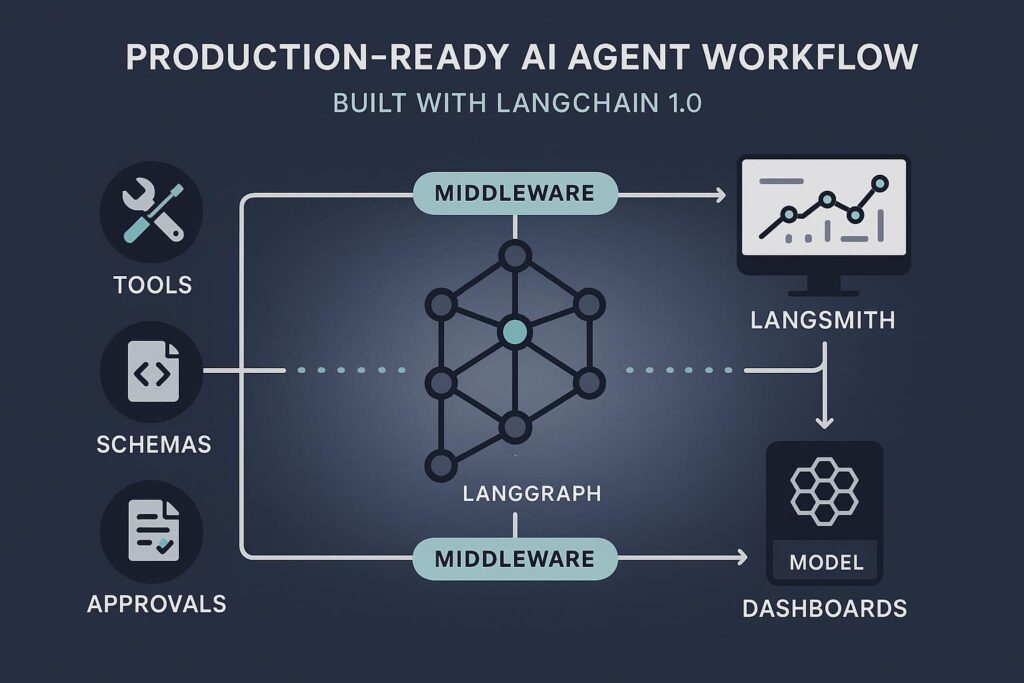
\includegraphics[width=0.5\textwidth]{Images/system/lang_mid.jpg}
    \vspace{12pt}\caption{Practice of Langchain Middleware Integration, inspired by \href{https://skywork.ai/blog/ai-agent/best-practices-langchain-1-0-production-ready-llm-apps/}{How LangChain 1.0 Simplifies Building Production-Ready LLM Applications}}}\label{fig:lang_mid}
\end{figure}
Langchain Middleware~\cite{LangMid}, released in December 2025, is one of the latest features providing a composable interceptor that modifies the model's request before it reaches the language model, 
enabling a single agent to exhibit distinct behaviours per workflow node. Unlike role-based frameworks where changing an agent's behaviour requires spawning 
a new instance entirely, the middleware approach eliminates redundant model connections while preserving per-node specialisation. The Figure~\ref{fig:lang_mid} 
demonstrates the reference to the practice of LangChain Middleware Integration.

\subsection{LangGraph Workflow Design}

The TA Module's orchestration layer is built as a LangGraph state machine where each node represents either a specialised processing step or a compiled sub-workflow. 
For each node design, the components within the schema orchestrate data flow through two primary mechanisms. As the agent state and student state traverse 
the nodes alongside runtime configurations, an exclusion mechanism is applied: the system filters the context so that each agent only sees the information strictly necessary for its current task, keeping the prompt clean and preventing interference from irrelevant data.
\begin{figure}[H]
    \centering
    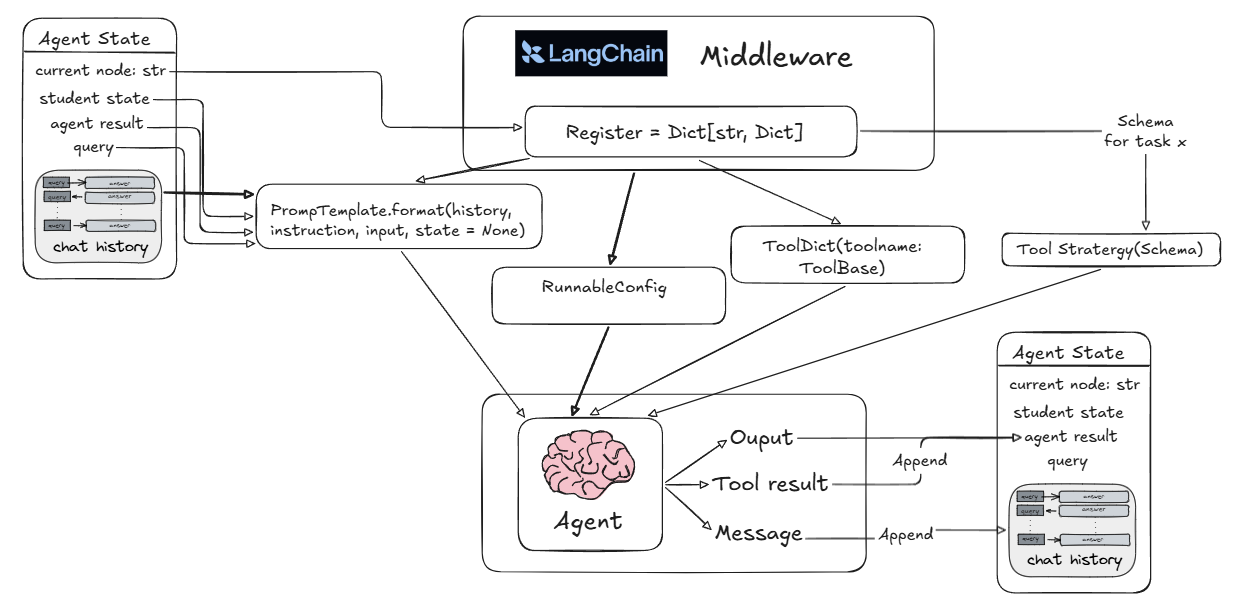
\includegraphics[width=\textwidth]{Images/system/langchain_node.png}
    \vspace{12pt}\caption{Standard operation of a LangGraph Node}\label{fig:lang_node}
\end{figure}
\paragraph*{AgentState:} Representing the dynamic data payload and memory of the system.
\begin{itemize}
  \item Query: Input from the user
  \item Agent result: Other Agents non message results accumulated from previous nodes in the workflow such as intermediate reasoning, tool results buffer.
  \item Chat history: An array containing the conversation history results.
  \item Current Node: name of the current node, used to find its pre\-registered means and resources in the Register
\end{itemize}

\paragraph*{Middleware:} Building upon the core middleware framework, the system applies the Adaptive Middleware pattern inherited from Langchain. My design ties its
behaviour with the Register, which is a nested dictionary. The LangGraph Node name act as a key to access an inner dictionary containing the following items:
\begin{itemize}
  \item Prompt Template: Created by LangChain PromptTemplate. Constructs AgentState and Query by combining predefined Meta Context and task instruction, 
  forming a detailed instruction set to invoke agents. For TA, the Prompt template include chat history and optionally agent result
  \item Tools: Grouped according to task and registered during initialization.
  \item ToolStrategy: Override schema runtime during
  \item Runnable Config: Registered configurations that change agent behaviour according to the task. For example, enforcing low temperatures for rigid retrieval tasks.
\end{itemize}
The Middleware use the node name to get the dictionary, then pass it to the built\-in Langchain call() method overriding agent calls, redefining agent behaviour and output.
Agent output will append to Agent State as in the figure. This ensure state and context management across the whole workflow, while still preserve local context and agentic
behaviour in that local setting.


% ─────────────────────────────────────────────────────────────────────────────

% ─────────────────────────────────────────────────────────────────────────────
\subsection{Tracing and Observability}\label{sub:tracing}
% ─────────────────────────────────────────────────────────────────────────────

Agentic systems is an unstable and blackbox pipeline. Ensuring system in production requires comprehensive observability of agentic input, output and all intermediate step including reasoning chain 
to diagnose reasoning failures, measure latency bottlenecks, and audit the decision-making process. The Tracing Module captures a structured record of every agent 
interaction, providing both local persistence for debugging and long-term monitoring.

The tracing system organises observability data into a three-level hierarchy, illustrated in Figure~\ref{fig:trace_model}. Each level captures progressively finer-grained information about the agent's execution.

\begin{figure}[H]
\centering
\begin{tikzpicture}[
  level/.style={draw, rounded corners=3pt, minimum width=3.0cm, minimum height=0.7cm, align=center, font=\small, fill=#1},
  arr/.style={->, >=stealth, thick},
  contains/.style={font=\tiny, midway, right},
]
\node[level=blue!15] (session) at (0, 2) {Trace Session};
\node[level=orange!12] (chat) at (0, 0.5) {Chat Trace};
\node[level=green!12] (step) at (0, -1) {Step Trace};
\draw[arr] (session) -- node[contains]{contains many} (chat);
\draw[arr] (chat) -- node[contains]{contains many} (step);
% Fields
\node[font=\tiny, anchor=west, text=gray] at (2.0, 2.3) {session id, schema version};
\node[font=\tiny, anchor=west, text=gray] at (2.0, 0.8) {chat id, query, intent, final output, status};
\node[font=\tiny, anchor=west, text=gray] at (2.0, -0.7) {node name, prompt snapshot, student state,};
\node[font=\tiny, anchor=west, text=gray] at (2.0, -1.1) {tool results, LLM output};
\end{tikzpicture}
    \vspace{12pt}\caption{Trace data hierarchy. Three nested observation levels.}\label{fig:trace_model}
\end{figure}

At the top level, a Trace Session spans the student's entire connected session and serves as the root container. Each student message creates a Chat Trace 
containing the original query, the classified intent, and the final response. Within each chat, Step Traces record the execution of each workflow node: 
the prompt to invoke language model (truncated for context window fit and storage effieciency), a snapshot of the AgentState at that moment containing 
student's learning state , any tool execution results, and the model's output.

Each active session maintains an in-memory trace buffer. As workflow nodes execute, each node appends a step record to the current chat's buffer. When a chat turn 
completes, the full session trace is serialised to JSON and written to a persistent file. The writer employs dual locking mechanisms---a threading lock for synchronous 
contexts and an asynchronous lock for coroutine contexts---ensuring thread safety when multiple workflow nodes attempt concurrent trace writes.

For production monitoring, the system integrates with Langfuse, a cloud-based observability platform built for LLM applications. 
The integration operates through LangChain's callback protocol: a Langfuse callback handler is injected into the runtime configuration at a 
session starts, automatically capturing every LLM invocation, tool call precisely from inner system.
\newpage
\chapter{Experiment}
Following the development phase, the core backbone engine has been successfully implemented. This chapter presents the operational results of the system architecture discussed previously. Specifically, each logical module exposes dedicated API endpoints to handle application requests. Furthermore, the underlying infrastructure has been robustly deployed, ensuring a seamless environment for the application to function.

\section{Application Deployment}
\subsection{Database Setup}
The initialization of Docker containers was executed successfully, establishing the foundational database infrastructure.

\begin{figure}[H]
    \centering
    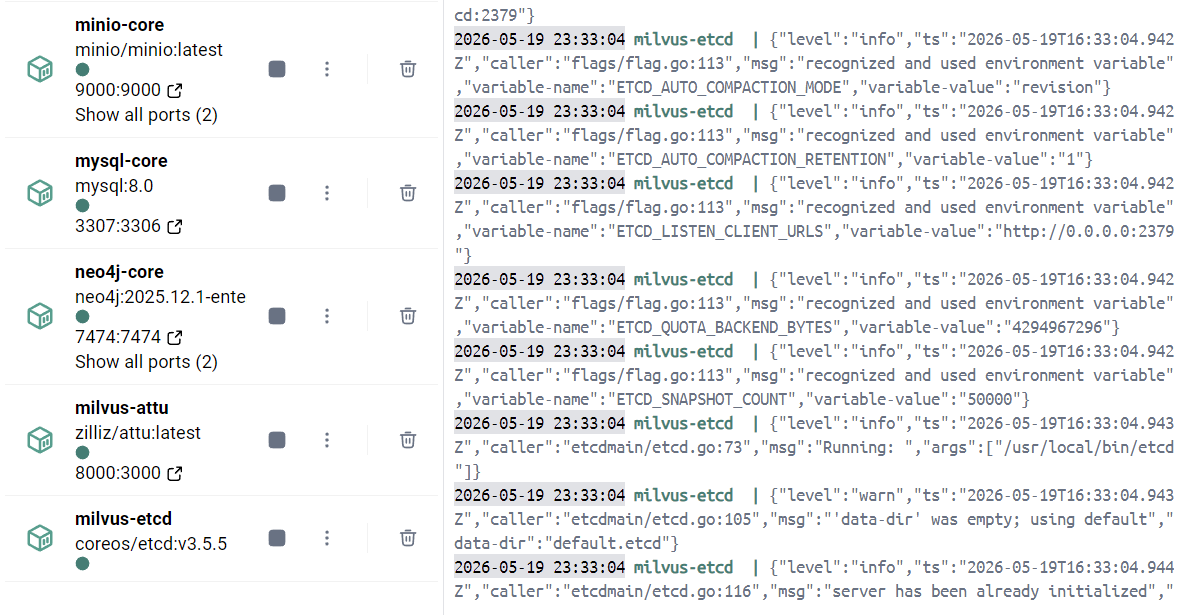
\includegraphics[width=\textwidth]{Images/ex/docker.png}
    \vspace{12pt}\caption{Docker-base infrastructure containerization and deployment}\label{fig:db_infra}
\end{figure}

Additionally, the system provides comprehensive database monitoring tools for all data containers, facilitating efficient debugging and direct tool testing.

\begin{figure}[H]
    \centering
    \begin{minipage}{0.25\textwidth}
        \centering
        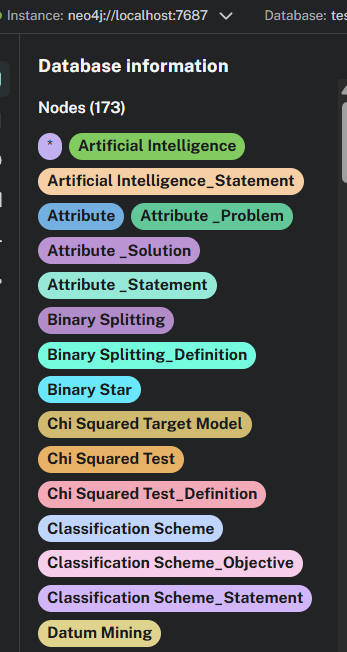
\includegraphics[width=\linewidth]{Images/ex/neo.png}
        \vspace{8pt}\caption{Neo4j Monitor Plugins}
    \end{minipage}\hfill
    \begin{minipage}{0.6\textwidth}
        \centering
        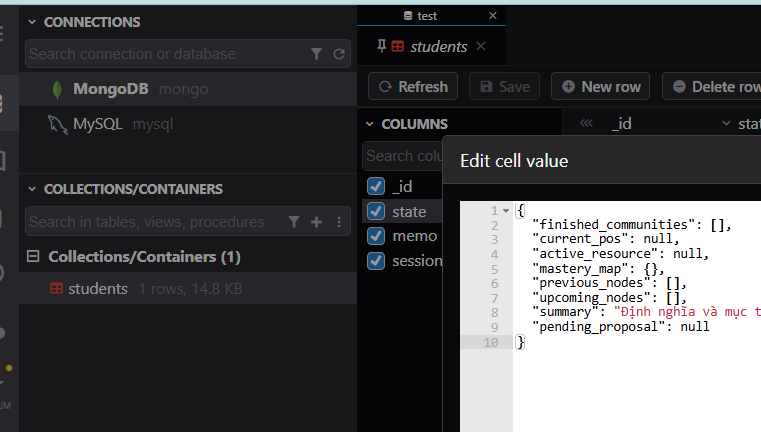
\includegraphics[width=\linewidth]{Images/ex/dbgate.png}
        \vspace{8pt}\caption{DBgate monitoring both MongoDB and SQLite}
    \end{minipage}
    \vspace{12pt}\caption{Database Admin Monitoring and Visualizing}\label{fig:db_monitor}
\end{figure}

\subsection{FastAPI App Deployment}
\begin{figure}[H]
    \centering
    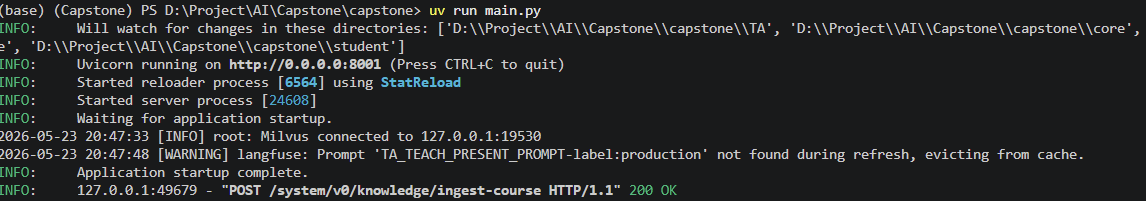
\includegraphics[width=\textwidth]{Images/ex/app_run.png}
    \vspace{12pt}\caption{FastAPI successful lifecycle start}\label{fig:app_run}
\end{figure}
The App is hosted via uvicorn. The lifespan create connection pool, initialize Singleton Modules and listen on port 8001. The Figure~\ref{fig:app_run} 
shows that all deployments are success and endpoints of main components have been publicly exposed for usage.
\section{Knowledge Module}
\subsection{Service Endpoints}
\begin{itemize}
    \item {\texttt{POST /ingest-course}}
    \begin{itemize}
        \item {Use case}: Enqueues a course ingestion request, validates the presence of uploaded PDF documents, and triggers the background processing pipeline to extract semantic concepts and construct the Knowledge Graph.
        \item {Input schema}: 
        \begin{itemize}
            \item \texttt{course\_name} (String): The title of the course being ingested.
            \item \texttt{slide\_files} (List of Strings): A list of slide file names to be processed.
            \item \texttt{textbook\_files} (List of Strings): A list of textbook file names to be processed.
            \item \texttt{reset} (Boolean): A flag indicating whether to reset the existing course data before proceeding.
        \end{itemize}
        \item {Output schema}: 
        \begin{itemize}
            \item \texttt{status} (String): The acceptance status of the background task.
            \item \texttt{message} (String): A descriptive confirmation message.
            \item \texttt{details} (Object): Additional metrics, including the count of slides and textbooks queued.
        \end{itemize}
    \end{itemize}
\end{itemize}

\subsection{Runtime}
During execution, the client transmits documents via an HTTP stream of bytes, which are subsequently loaded as PDF files. 
\begin{figure}[H]
    \centering
    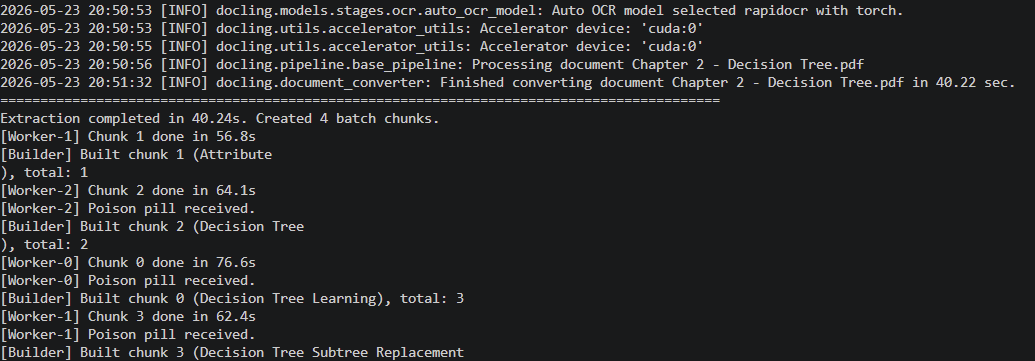
\includegraphics[width=\textwidth]{Images/ex/asynch_ingest.png}
    \vspace{12pt}\caption{Tracking Log of Asynchronous Ingestion}\label{fig:asynch_ingest}
\end{figure}
Those file goes through an asynchronous, long extraction process to formulating normalized filtered nodes and edges.

\begin{figure}[H]
    \centering
    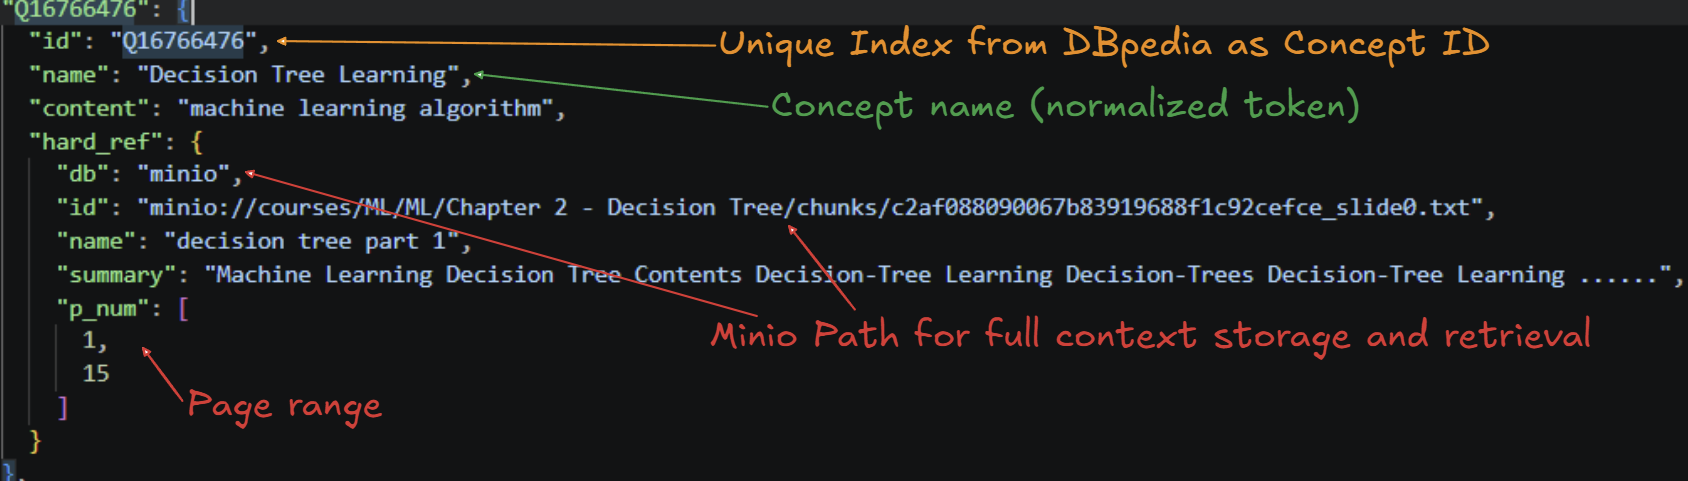
\includegraphics[width=\textwidth]{Images/ex/node.png}
    \vspace{12pt}\caption{Extracted Concept Nodes}\label{fig:node_dict}
\end{figure}
All those valuable Artifacts are pushed and saved on Neo4J. 
\begin{figure}[H]
    \centering
    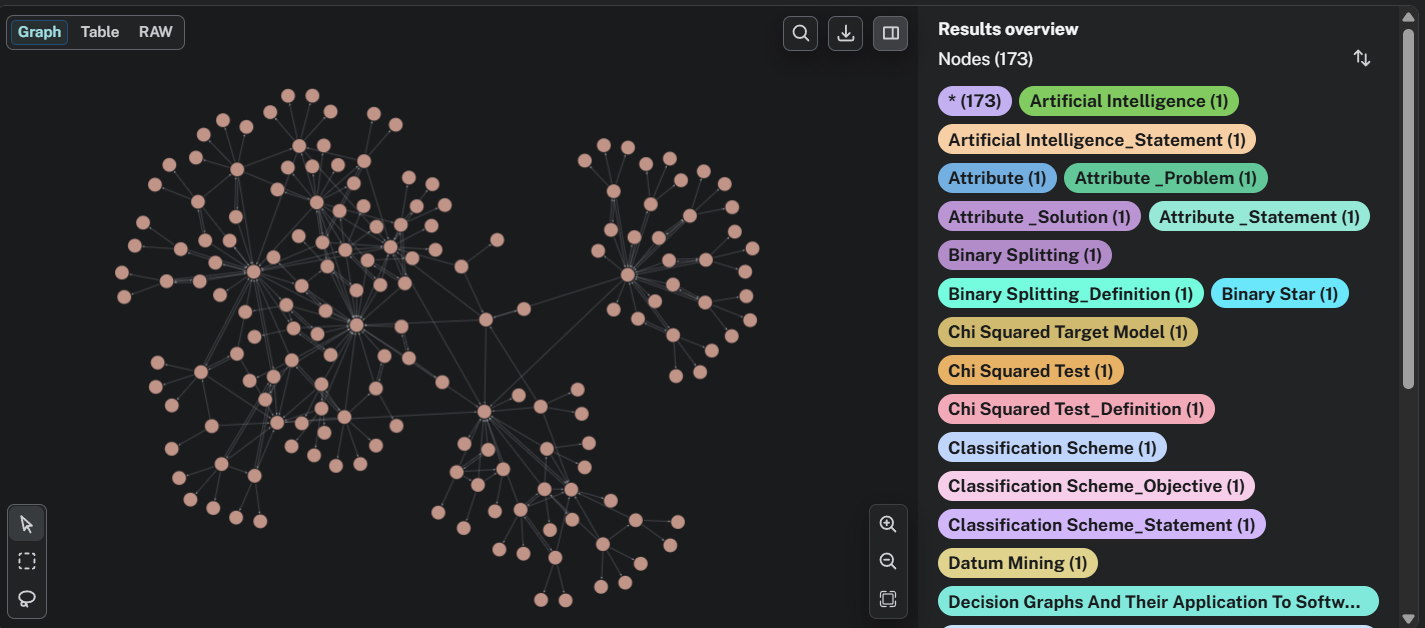
\includegraphics[width=\textwidth]{Images/ex/graph.png}
    \vspace{12pt}\caption{Completed Knowledge Graph demonstrating no concept fragmentation}\label{fig:graph_neo}
\end{figure}

However, the external knowledge base, DBpedia, occasionally provides inconsistent name and definitions. 
This manifests as words receiving inaccurate definitions or unnormalized representations.

\begin{figure}[H]
    \centering
    
\includegraphics[width=0.3\textwidth]{Images/ex/pedia_err.png}
    \vspace{12pt}\caption{DBpedia accepting unusual or unnormalized node names}\label{fig:pedia_err}
\end{figure}

Furthermore, we observed the following operational constraints:
\begin{itemize}
    \item An overly detailed Knowledge Graph becomes challenging to visualize, especially when exceeding 100 nodes and generating over 300 relationships per 20 pages.
    \item The ingestion process requires approximately 250 seconds per 50 pages, even when utilizing 3 asynchronous task workers.
\end{itemize}

\section{Student Module}
\subsection{Service Endpoints}
The Student Module exposes several key endpoints for identity and session management:

\begin{itemize}
    \item {\texttt{POST /register}}
    \begin{itemize}
        \item {Use case}: Registers new student profiles, hashes credentials, and initializes a default state document.
        \item {Input schema}:
        \begin{itemize}
            \item \texttt{student\_id} (String): The unique identifier chosen by the student.
            \item \texttt{password} (String): The plain-text password to be securely hashed.
        \end{itemize}
        \item {Output schema}:
        \begin{itemize}
            \item \texttt{detail} (String): Confirmation message of successful registration.
        \end{itemize}
    \end{itemize}

    \item {\texttt{POST /login}}
    \begin{itemize}
        \item {Use case}: Validates student credentials and generates a secure JWT authentication payload.
        \item {Input schema}:
        \begin{itemize}
            \item \texttt{username} (String): The student's unique identifier.
            \item \texttt{password} (String): The student's password.
        \end{itemize}
        \item {Output schema}:
        \begin{itemize}
            \item \texttt{access\_token} (String): The JWT payload used for subsequent authenticated requests.
            \item \texttt{token\_type} (String): The token category, typically set to "bearer".
        \end{itemize}
    \end{itemize}

    \item {\texttt{POST /session/start}}
    \begin{itemize}
        \item {Use case}: Generates a session-specific UUID token to isolate chat interactions.
        \item {Input schema}:
        \begin{itemize}
            \item \texttt{Authorization} (Header String): Bearer token (JWT) of the authenticated student.
        \end{itemize}
        \item {Output schema}:
        \begin{itemize}
            \item \texttt{session\_id} (String): A uniquely generated UUID functioning as an opaque token for a specific chat instance.
        \end{itemize}
    \end{itemize}

    \item {\texttt{DELETE /session/end}}
    \begin{itemize}
        \item {Use case}: Discards the active session token to cleanly terminate the session.
        \item {Input schema}:
        \begin{itemize}
            \item \texttt{session\_id} (Query String): The UUID of the session to terminate.
            \item \texttt{Authorization} (Header String): Bearer token (JWT) of the authenticated student.
        \end{itemize}
        \item {Output schema}: Returns HTTP 204 (No Content) indicating successful deletion.
    \end{itemize}
\end{itemize}

\subsection{Runtime}
The system demonstrates the capability to robustly handle user sessions, including detecting pre-existing users during registration or login processes.

\begin{figure}[H]
    \centering
    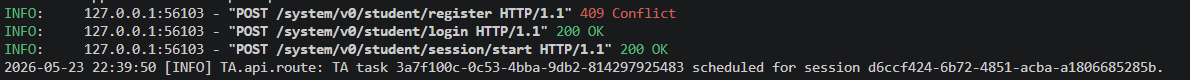
\includegraphics[width=\textwidth]{Images/ex/login.png}
    \vspace{12pt}\caption{Status 409 indicating a pre-existing student ID entry in the database. A new Session ID and access credentials are concurrently created.}\label{fig:session_login}
\end{figure}

\section{Teaching Module}
\subsection{Service Endpoints}
\begin{itemize}
    \item {\texttt{POST /chat}}
    \begin{itemize}
        \item {Use case}: Serves as the primary tutoring interface. It receives user queries alongside their active session IDs, subsequently executing the multi-agent LangGraph tutoring pipelines to formulate contextual responses.
        \item {Input schema}:
        \begin{itemize}
            \item \texttt{session\_id} (String): The UUID for the active chat session authenticated by the user.
            \item \texttt{user\_input} (String): The actual query or message submitted by the student.
            \item \texttt{language} (String): The language preference toggle (e.g., "vn" or "eng").
        \end{itemize}
        \item {Output schema}:
        \begin{itemize}
            \item \texttt{task\_id} (String): A unique identifier assigned to track the asynchronous background task.
            \item \texttt{status} (String): The initial state, typically indicating receipt of the request.
            \item \texttt{agent} (String): The default agent assigned to process the workflow.
        \end{itemize}
    \end{itemize}

    \item {\texttt{GET /chat/status/\{task\_id\}}}
    \begin{itemize}
        \item {Use case}: Sends system status back to the client while waiting. The streaming output can be included here as well.
        \item {Input schema}:
        \begin{itemize}
            \item \texttt{task\_id} (Path String): The unique identifier of the background task being polled.
        \end{itemize}
        \item {Output schema}:
        \begin{itemize}
            \item \texttt{status} (String): The current operational state (e.g., "working", "finished", or "Fail").
            \item \texttt{agent\_name}, \texttt{intent}, \texttt{thought} (String, optional): Metadata illustrating the agent's current step, intended action, and reasoning.
            \item \texttt{result} (Object, optional): Available upon completion, containing the final \texttt{message} string and optional \texttt{ui\_action} dictionaries.
            \item \texttt{error} (String, optional): Descriptive failure logs in the event of pipeline exceptions.
        \end{itemize}
    \end{itemize}
\end{itemize}
\subsection{Runtime}
Upon submitting a query, the client interface consistently monitors the agentic progress, displaying the current status and the active agent. Once the pipeline concludes, the service transmits the final text result back to the client.

\begin{figure}[H]
    \centering
    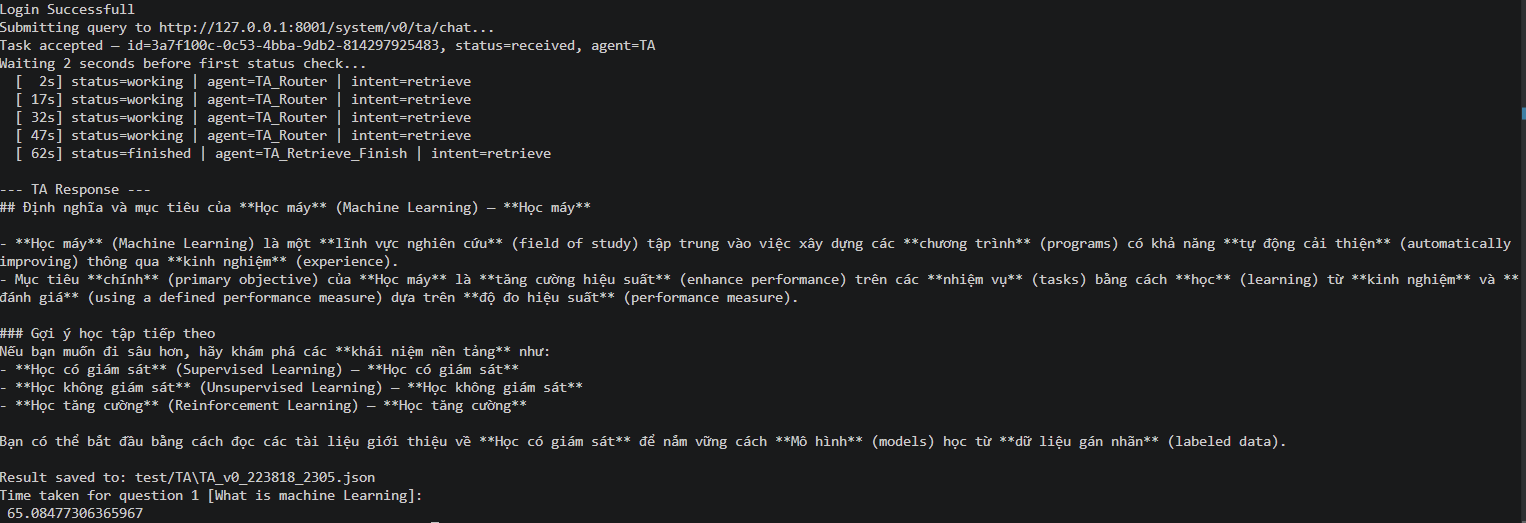
\includegraphics[width=\textwidth]{Images/ex/full_TA_output_1.png}
    \vspace{12pt}\caption{Client-side interface displaying the agentic interaction flow}\label{fig:client_answer}
\end{figure}

Simultaneously, the system persistently logs and saves the outcomes of agentic tool executions and messages, facilitating potential reusability and analytical reviews.

\begin{figure}[H]
    \centering
    \begin{minipage}{0.48\textwidth}
        \centering
        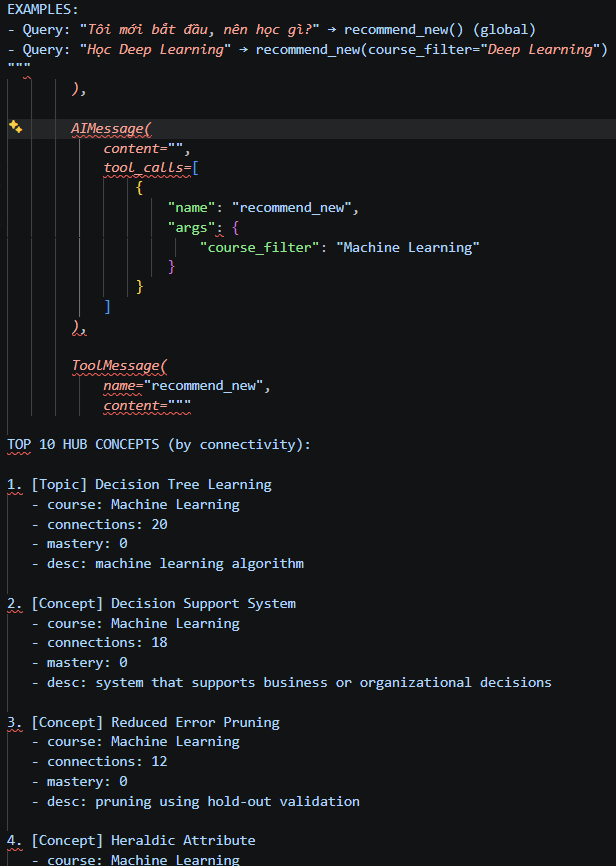
\includegraphics[width=\linewidth]{Images/ex/tool_mess.png}
    \end{minipage}\hfill
    \begin{minipage}{0.48\textwidth}
        \centering
        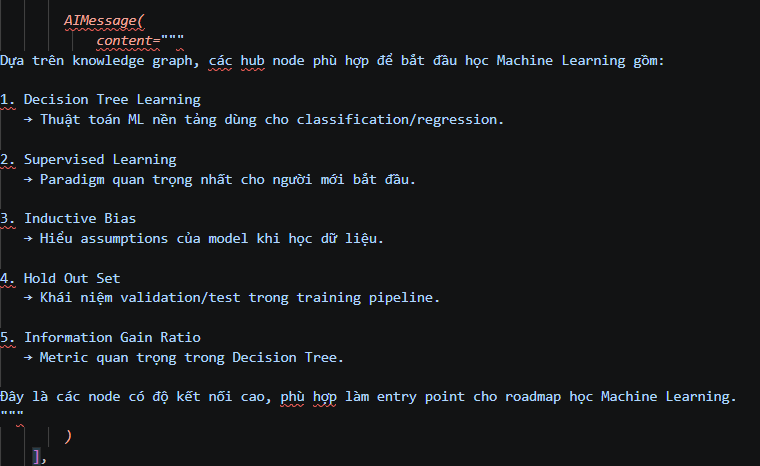
\includegraphics[width=\linewidth]{Images/ex/ai_mess.png}
    \end{minipage}
    \vspace{12pt}\caption{2 snippet of Logged Agent Workflow result}\label{fig:workflow_log}
\end{figure}

Currently, the core teaching workflow remains under active development, while the retrieval and roadmap workflows have
 demonstrated promising initial results. Moving forward, comprehensive benchmarks and advanced evaluation metrics will 
 be investigated to formally assess the system's efficiency in automated, intelligent education expertise.
\newpage
\chapter{Conclusion}

\section{Achieved Results}
The integration of the SmartEdu system has successfully demonstrated a working, agent-driven educational platform. By focusing on practical functionality and stable outputs, the system has achieved the following results:

\begin{itemize}
    \item {Unified Knowledge Graph:} The system automatically builds a connected and non-fragmented Knowledge Graph. Concepts remain consistent throughout the course, providing a reliable database for all agent tasks.
    \item {Consistent AI Operations:} Guided by state-based harnessing, the multi-agent system runs stably. It reliably retrieves data, maps out learning roadmaps, and identifies backbone concepts without hallucinating or drifting off-topic.
    \item {Scalable System Design:} The backend architecture is modular and separates state management from AI processing, making it ready to scale into a microservices environment.
    \item {Multimodal Input Processing:} The platform successfully preserves the structural layouts and visual references of the original materials, allowing agents to "read" and utilize this rich context for better answers.
    \item {Reliable Error Handling:} The system includes a robust fallback mechanism. When specific context is missing, the agents safely switch to exploring the broader graph instead of generating fake information.
\end{itemize}

\section{System Limitations}
Despite its functional success, the current version of the system has several practical limitations that affect its speed and long-term usability:

\begin{itemize}
    \item {Unclear Course-Level Paths:} Defining prerequisites for an entire course is still difficult. The exact threshold for deciding when to merge overlapping topics remains undecided, which can cause confusion in the macro-roadmap.
    \item {Lack of Self-Improvement:} The system's intelligence comes from static, specialized prompts (the harness), not the models themselves. The agents cannot learn from their own mistakes, meaning the system is not yet truly adaptive.
    \item {High Latency:} Processing time is a major bottleneck. A simple data retrieval takes up to 30 seconds, while complex tasks like generating a roadmap or a teaching response can take up to 60 seconds.
    \item {Limited Long-Term Tracking:} The context from which Teaching Assistant assesses situation are still tied to the present chat session. 
    It currently lacks a reliable way to track and evaluate a student's progress over a long period.
    \item {Incomplete Application:} The frontend interface is not developed, and the application is still not hosted, limiting how users can visually interact 
    with the system and their roadmaps.
\end{itemize}

\section{Future Plan}
To prepare the SmartEdu system for final deployment and defense, the remaining work is scheduled into an 8-week execution plan. 
This focuses on visual interfaces, speed optimization, and final testing:

\begin{enumerate}
    \item \textbf{Weeks 1: Completion of Agentic Design on a Macro Scale} Improve agentic module performance for more challenging cases. 
    Propose reliable metrics.
    \item \textbf{Weeks 2: Interactive UI/UX Design.} Build the frontend interface and and test system deployments. Provide addtional features:
    \begin{itemize}
        \item Let students visually navigate the Knowledge Graph, view their roadmaps dynamically, and chat easily with the system.
        \item Streamline output to reduce response latency, display original PDF file with highlighter for deeper knowledge comprehension
    \end{itemize}
    
    \item \textbf{Weeks 3--4: Student Tracking and Exercises.} Add interactive exercises and a reliable scoring and evaluation system for student. Using these academic records, the system will apply clustering algorithms to group students with similar learning patterns for better long-term tracking.

    \item \textbf{Weeks 5--6: Optimization of Agent components on a Micro Scale } Improve Agentic Memory, Algorithm construction and speed up inference. 
    This step aims to cut down the current 30--60, while still improving quality.
    
    
    \item \textbf{Weeks 7--8: System Benchmarking and Final Report.} Run practical tests to evaluate the TA's accuracy and its impact on students. 
    Finally, summarize all results into the graduation thesis and prepare the visual presentation for the defense.
\end{enumerate}
\newpage
%%%%%%%%%%%%%%%%%OUTRO%%%%%%%%%%%%%%%%%%%
\bibliographystyle{plain}
\bibliography{References}
\nocite{*}


%Warning--entry type for "oath" isn't style-file defined
%--line 10 of file References.bib
%Warning--entry type for "docker_docs" isn't style-file defined
%--line 18 of file References.bib
%Warning--entry type for "aws_docs" isn't style-file defined
%--line 26 of file References.bib

\end{document}


